\documentclass{article}

% if you need to pass options to natbib, use, e.g.:
%     \PassOptionsToPackage{numbers, compress}{natbib}
% before loading neurips_2024


% ready for submission
\usepackage{neurips_2024}


% to compile a preprint version, e.g., for submission to arXiv, add add the
% [preprint] option:
%     \usepackage[preprint]{neurips_2024}


% to compile a camera-ready version, add the [final] option, e.g.:
%     \usepackage[final]{neurips_2024}


% to avoid loading the natbib package, add option nonatbib:
%    \usepackage[nonatbib]{neurips_2024}


\usepackage[utf8]{inputenc} % allow utf-8 input
\usepackage[T1]{fontenc}    % use 8-bit T1 fonts
\usepackage{hyperref}       % hyperlinks
\usepackage{url}            % simple URL typesetting
\usepackage{booktabs}       % professional-quality tables
\usepackage{amsfonts}       % blackboard math symbols
\usepackage{nicefrac}       % compact symbols for 1/2, etc.
\usepackage{microtype}      % microtypography
\usepackage{xcolor}         % colors


\usepackage{amsmath}
\usepackage{amssymb}
\usepackage{amsthm}
\usepackage{mathtools}
\usepackage{tikz}
\usetikzlibrary{arrows.meta,positioning,calc}

\providecommand{\R}{\mathbb{R}}
\providecommand{\E}{\mathbb{E}}
\providecommand{\FIM}{\mathcal{F}}
\providecommand{\norm}[1]{\lVert #1 \rVert}

\providecommand{\abs}[1]{\lvert #1 \rvert}
\providecommand{\inner}[2]{\langle #1, #2 \rangle}

\DeclareMathOperator{\diag}{diag}
\DeclareMathOperator{\tr}{tr}
\DeclareMathOperator{\Var}{Var}
\DeclareMathOperator{\Cov}{Cov}
\DeclareMathOperator{\rank}{rank}
\DeclareMathOperator{\srank}{srank}

\theoremstyle{plain}
\newtheorem{theorem}{Theorem}
\newtheorem{lemma}{Lemma}
\newtheorem{proposition}{Proposition}
\newtheorem{corollary}{Corollary}
\newtheorem{assumption}{Assumption}
\theoremstyle{definition}
\newtheorem{definition}{Definition}
\theoremstyle{remark}
\newtheorem{remark}{Remark}

\title{Geometric Plasticity: How Natural Gradient Descent Mitigates Loss of Plasticity \\ via Spectral Normalization and Curvature Preservation}

\author{%
  Author One\\
  Department of Computer Science\\
  University of Plasticity\\
  Location, Country\\
  \texttt{email@domain.edu}
  \And
  Author Two\\
  Department of Computer Science\\
  University of Plasticity\\
  Location, Country\\
  \texttt{email@domain.edu}
}

\begin{document}
\small

\maketitle

%==============================================================
% ABSTRACT
%==============================================================
\begin{abstract}
Neural networks trained on non-stationary data streams suffer from \emph{Loss of Plasticity} (LoP): the progressive degradation of their ability to learn new tasks. Recent theory identifies two structural barriers---\emph{frozen units} and \emph{cloned units}---as stable invariant manifolds from which SGD cannot escape. We analyze \emph{Natural Gradient Descent} (NGD), via K-FAC, as a plasticity maintainer, proving three results with quantified assumptions and explicit limitations:
(1)~NGD equalizes per-direction convergence rates; we extend this beyond the quadratic case via a \emph{semi-global tracking theorem} with explicit cross terms, and partially bound the Kronecker approximation error $\epsilon_K$ that governs equalization quality;
(2)~for near-frozen and near-cloned units, we prove quantifiable NGD/SGD amplification ratios at fixed damping, with explicit conditions guaranteeing the perpendicular gradient fraction $c_\perp > 0$ (Lemma~\ref{lem:c_perp});
(3)~we prove bounded weight dynamics via both a global Lyapunov analysis (three architecture classes with verified constants) and a \emph{per-layer} analysis that resolves the exponential depth blowup for deep ReLU networks. Experiments on ResNet-18 confirm zero dormant units under K-FAC while SGD and CBP exhibit monotonically increasing dormancy.
To extend these guarantees to architectures \emph{without} BatchNorm (e.g., plain MLPs), we further propose two \emph{implicit BatchNorm} mechanisms integrated directly into the K-FAC optimizer---\textbf{OPC} (Online Pre-activation Centering) and \textbf{CWN} (Centered Weight Normalization)---that replicate BN's mean-centering and zero-mean-weight properties, respectively, without any architectural modification.
\end{abstract}

%==============================================================
% 1. INTRODUCTION
%==============================================================
\section{Introduction}
\label{sec:intro}

Continual learning demands that neural networks sequentially acquire new knowledge while retaining previously learned capabilities. While catastrophic forgetting---the loss of past knowledge---has been studied extensively \citep{kirkpatrick2017ewc}, a complementary and arguably more fundamental failure mode has recently attracted intense scrutiny: \emph{Loss of Plasticity} (LoP) \citep{dohare2024loss, lyle2023understanding}. LoP refers to the phenomenon whereby a network's ability to minimize training error on \emph{new} tasks deteriorates progressively, even when the network possesses sufficient representational capacity.

The seminal work of \citet{dohare2024loss}, published in \emph{Nature}, demonstrated that standard backpropagation with SGD inevitably loses plasticity on long task sequences, eventually performing no better than a shallow linear model. This finding has sparked a wave of research investigating both the mechanisms and mitigations of LoP across supervised learning \citep{lewandowski2025spectral, farias2025snr, shin2024dash}, reinforcement learning \citep{sokar2023dormant, nikishin2023plasticity, juliani2024plasticity, tang2025mitigating}, and multi-agent settings \citep{qin2024reborn}.

\paragraph{Mechanistic understanding of LoP.} Several complementary theoretical frameworks have emerged. \citet{lyle2023understanding} linked plasticity loss to changes in loss landscape curvature. \citet{sokar2023dormant} identified the accumulation of \emph{dormant neurons} as a key correlate. Most recently, \citet{joudaki2026barriers} provided a dynamical systems perspective, proving that LoP manifests as entrapment in stable invariant manifolds characterized by either \emph{frozen units} (vanishing pre-activations) or \emph{cloned units} (duplicate weight vectors causing rank collapse). Independently, \citet{he2025spectral} showed that \emph{Hessian spectral collapse}---the vanishing of meaningful curvature directions---is the proximal cause of LoP, introducing the concept of $\tau$-trainability.

\paragraph{Existing mitigations.} Current approaches overwhelmingly rely on explicit architectural interventions: periodic neuron reinitialization \citep{sokar2023dormant, farias2025snr}, plasticity injection \citep{nikishin2023plasticity}, shrink-and-perturb \citep{ash2020warm, juliani2024plasticity}, spectral regularization \citep{lewandowski2025spectral}, churn reduction \citep{tang2025mitigating}, utility-based perturbation \citep{elsayed2024upgd}, regenerative regularization \citep{kumar2025l2init}, and rank-preserving weight decay \citep{wu2026rank}. These methods treat LoP symptoms post-hoc. A natural question arises:

\begin{center}
\emph{Can the optimization algorithm itself prevent Loss of Plasticity?}
\end{center}

\paragraph{Our contribution.} We answer affirmatively by analyzing \emph{Natural Gradient Descent} (NGD) \citep{amari1998natural} through the lens of its K-FAC approximation \citep{martens2015optimizing}. Traditionally viewed as a convergence accelerator, NGD optimizes along geodesics of the statistical manifold defined by the Fisher Information Matrix (FIM). We show that this geometric structure endows NGD with four properties that directly counter the known mechanisms of LoP:

\begin{enumerate}
    \item \textbf{Spectral Equalization} (Theorems~\ref{thm:spectral}--\ref{thm:tracking}, Lemma~\ref{lem:epsilon_K}): K-FAC achieves perfect condition ratio in the quadratic case. For nonlinear networks under distribution shift, our semi-global tracking theorem bounds the condition ratio via $\eta$ with \emph{explicit cross terms} in the Kronecker product perturbation. We partially resolve the $\epsilon_K$ gap with Lemma~\ref{lem:epsilon_K}, characterizing when the Kronecker factorization is accurate ($O(1/\sqrt{m})$ for wide first layers, empirically small with BatchNorm).
    
    \item \textbf{Barrier Escape} (Theorems~\ref{thm:barrier}--\ref{thm:clone}, Lemma~\ref{lem:c_perp}): For near-frozen and near-cloned units, we prove amplification ratios at \emph{fixed} $\gamma > 0$. The new Lemma~\ref{lem:c_perp} provides explicit conditions guaranteeing the perpendicular gradient fraction $c_\perp > 0$ (generically almost surely for Gaussian data), resolving the previously unquantified ``$g_\perp$ is nontrivial'' assumption.
    
    \item \textbf{Bounded Weight Dynamics} (Theorems~\ref{thm:lyapunov_layer}--\ref{thm:lyapunov}, Lemma~\ref{lem:verify}): We verify the bounded natural gradient assumption for three architecture classes. For deep ReLU networks where the global $M_2$ blows up exponentially, we introduce a \emph{per-layer Lyapunov analysis} (Theorem~\ref{thm:lyapunov_layer}) showing that each layer's K-FAC update norm does not depend on its own Frobenius norm, giving $m_{2,l} = 0$ and unconditional contraction under any positive weight decay.
    
    \item \textbf{Weight Norm Monotone Contraction} (Theorem~\ref{thm:weight_contraction}): For scale-invariant architectures (ResNet + BatchNorm), we prove that K-FAC + weight decay induces \emph{geometric (exponential) weight norm contraction} with no positive equilibrium---in sharp contrast to SGD, where weight norms stabilize at a positive equilibrium. This explains the empirically observed persistent decrease of weight magnitudes under K-FAC and identifies it as a fourth mechanism countering LoP.

    \item \textbf{Implicit BatchNorm for Plain MLPs} (\S\ref{subsec:implicit_bn}): For architectures \emph{without} BN, we propose two optimizer-level mechanisms integrated as post-step operations in K-FAC, requiring no architectural change:
    \begin{itemize}
        \item \textbf{OPC} (Online Pre-activation Centering): nudges each hidden bias toward zero mean pre-activation, countering ReLU neuron death and replicating BN's mean subtraction.
        \item \textbf{CWN} (Centered Weight Normalization): zero-centers each output-row of $W$, replicating BN's zero-mean-weight property and reinstating the gradient orthogonality that drives weight contraction.
    \end{itemize}
\end{enumerate}

Our work is the first to formally connect \emph{information geometry} to the structural barriers underlying LoP, establishing NGD as a principled, general-purpose plasticity maintainer rather than an ad-hoc fix.

%==============================================================
% 2. RELATED WORK
%==============================================================
\section{Related Work}
\label{sec:related}

\paragraph{Loss of Plasticity: Empirical evidence.}
The phenomenon of plasticity loss was systematically documented by \citet{dohare2024loss}, who showed on Permuted MNIST, Incremental CIFAR-100, and RL benchmarks that SGD-trained networks progressively degrade in their ability to fit new tasks. \citet{lyle2023understanding} provided an early analysis at ICML~2023, linking plasticity to loss landscape curvature properties in deep RL agents. \citet{sokar2023dormant} identified the \emph{dormant neuron phenomenon}---the accumulation of neurons with near-zero activation---as a key empirical correlate, particularly in off-policy RL. \citet{juliani2024plasticity} extended the study to on-policy settings at NeurIPS~2024, finding that many off-policy mitigations fail in the on-policy regime. The dormant neuron phenomenon was further studied in multi-agent settings by \citet{qin2024reborn} at NeurIPS~2024. \citet{shin2024dash} showed at NeurIPS~2024 that even in stationary settings, warm-started networks lose plasticity due to \emph{noise memorization}, proposing direction-aware shrinking (DASH) as a remedy.

\paragraph{Loss of Plasticity: Theoretical analysis.}
\citet{joudaki2026barriers} (ICLR~2026) provided the most complete theoretical treatment to date, casting LoP as entrapment in stable invariant manifolds of the gradient flow ODE. They identify two classes of barriers: \emph{frozen units} (neurons in the saturated regime of activations, yielding vanishing gradients) and \emph{cloned units} (neurons with identical weights, forming rank-deficient representations). Independently, \citet{he2025spectral} attributed LoP to \emph{Hessian spectral collapse}---the progressive loss of meaningful curvature directions---and introduced $\tau$-trainability as a unifying condition, proposing L2-ER (L2 regularization combined with effective rank maintenance) at ICLR~2026. \citet{wu2026rank} (ICLR~2026) characterized plasticity loss through NTK Gram matrix rank collapse and gradient magnitude decay of order $\Theta(1/k)$.

\paragraph{Mitigation strategies.}
The dominant paradigm involves explicit interventions. \textbf{Neuron resetting:} ReDo \citep{sokar2023dormant} reinitializes dormant neurons; Self-Normalized Resets \citep{farias2025snr} use hypothesis-testing-based thresholds at ICLR~2025; continual backpropagation \citep{dohare2024loss} randomly reinitializes low-utility units. \textbf{Regularization:} Spectral regularization \citep{lewandowski2025spectral} (ICLR~2025) keeps singular values near initialization; L2~Init \citep{kumar2025l2init} regularizes toward initial rather than zero weights; C-CHAIN \citep{tang2025mitigating} (ICML~2025) reduces churn to maintain NTK rank. \textbf{Perturbation:} Shrink-and-perturb \citep{ash2020warm} periodically contracts and perturbs weights; UPGD \citep{elsayed2024upgd} (ICLR~2024) applies utility-weighted perturbations; plasticity injection \citep{nikishin2023plasticity} (NeurIPS~2023) concatenates freshly initialized layers. In contrast to all these approaches, our work investigates whether the \emph{optimization geometry itself} can prevent LoP without explicit interventions.

\paragraph{Natural Gradient Descent and second-order methods.}
NGD \citep{amari1998natural} follows geodesics on the statistical manifold parameterized by the FIM. K-FAC \citep{martens2015optimizing} makes NGD practical via Kronecker-factored FIM approximation. Recent advances include SINGD \citep{lin2024singd} (ICML~2024), which provides an inverse-free, memory-efficient K-FAC variant; AdaFisher \citep{adafisher2025} (ICLR~2025), which bridges first- and second-order methods via block-Kronecker FIM approximation; and FOPNG \citep{garg2025fopng} (ICML~2025), which projects natural gradients onto Fisher-orthogonal complements for forgetting prevention. \citet{bernacchia2018exact} analyzed exact natural gradients in deep linear networks. On the theoretical side, \citet{zhao2024gn} (NeurIPS~2024) established tight bounds on the Gauss--Newton condition number in deep networks, \citet{doikov2024spectral} (ICML~2024) analyzed spectral preconditioning for graded non-convex functions, and \citet{xie2025structured} provided a unified regret analysis for Kronecker-structured preconditioners. Notably, while FOPNG uses the Fisher metric to prevent \emph{forgetting}, we show the Fisher metric inherently prevents \emph{plasticity loss}---addressing the complementary failure mode.

%==============================================================
% 3. PRELIMINARIES
%==============================================================
\section{Preliminaries}
\label{sec:prelim}

\subsection{Notation and Setup}

Consider a feedforward neural network with $L$ layers. For layer $l$, denote the weight matrix $W_l \in \R^{d_{l} \times d_{l-1}}$, the input activation vector $a_{l-1} \in \R^{d_{l-1}}$, and the pre-activation $z_l = W_l a_{l-1}$. The post-activation is $a_l = \sigma(z_l)$ for some activation function $\sigma$ (e.g., ReLU). We vectorize parameters as $\theta = \mathrm{vec}([W_1, \ldots, W_L]) \in \R^p$.

\subsection{Loss of Plasticity: Formal Definitions}

\begin{definition}[Loss of Plasticity \citep{dohare2024loss}]
\label{def:lop}
Let $\{\mathcal{T}_1, \mathcal{T}_2, \ldots\}$ be a sequence of tasks. A learning algorithm $\mathcal{A}$ operating on network $f_\theta$ exhibits \emph{Loss of Plasticity} if the training error achievable on task $\mathcal{T}_k$ after a fixed number of gradient steps increases with $k$:
\begin{equation}
    \E[\mathcal{L}_{\mathcal{T}_k}(\theta_k^*)] \geq \E[\mathcal{L}_{\mathcal{T}_k}(\theta_{k-1}^*)] + \delta_k, \quad \delta_k > 0,
\end{equation}
where $\theta_k^*$ is the parameter vector after training on task $\mathcal{T}_k$.
\end{definition}

\begin{definition}[Dormant Unit \citep{sokar2023dormant}]
\label{def:dormant}
Neuron $i$ in layer $l$ is $\epsilon$\emph{-dormant} with respect to data distribution $\mathcal{D}$ if
\begin{equation}
    \E_{x \sim \mathcal{D}}\left[\abs{\sigma(z_{l,i}(x))}\right] \leq \epsilon \cdot \frac{1}{d_l}\sum_{j=1}^{d_l} \E_{x \sim \mathcal{D}}\left[\abs{\sigma(z_{l,j}(x))}\right].
\end{equation}
\end{definition}

\begin{definition}[Frozen and Cloned Units \citep{joudaki2026barriers}]
\label{def:barriers}
For a ReLU network:
\begin{itemize}
    \item Unit $i$ in layer $l$ is \emph{frozen} if $\Pr_{x \sim \mathcal{D}}(z_{l,i}(x) \leq 0) = 1$, i.e., the unit is permanently inactive.
    \item Units $i, j$ in layer $l$ are \emph{cloned} if $w_{l,i} = c \cdot w_{l,j}$ for some scalar $c > 0$, yielding linearly dependent representations.
\end{itemize}
The sets of frozen configurations $\mathcal{M}_F$ and cloned configurations $\mathcal{M}_C$ form stable invariant manifolds of the SGD gradient flow.
\end{definition}

\subsection{Natural Gradient Descent with K-FAC}

The Fisher Information Matrix for a model $p_\theta(y|x)$ is:
\begin{equation}
    \FIM(\theta) = \E_{x \sim \mathcal{D}}\E_{y \sim p_\theta(\cdot|x)}\left[\nabla_\theta \log p_\theta(y|x) \nabla_\theta \log p_\theta(y|x)^\top\right].
\end{equation}
NGD updates parameters via $\theta_{t+1} = \theta_t - \eta \FIM(\theta_t)^{-1} \nabla_\theta \mathcal{L}(\theta_t)$.

\paragraph{K-FAC approximation.} For layer $l$ with input $a_{l-1}$ and output gradient $g_l = \nabla_{z_l}\mathcal{L}$, K-FAC \citep{martens2015optimizing} approximates the per-layer Fisher block as:
\begin{equation}
\label{eq:kfac}
    \FIM_l \approx A_{l-1} \otimes G_l,
\end{equation}
where $A_{l-1} = \E[a_{l-1} a_{l-1}^\top]$ is the input covariance and $G_l = \E[g_l g_l^\top]$ is the gradient covariance. In practice, damping is added: $\hat{\FIM}_l = A_{l-1} \otimes G_l + \gamma I$.

The per-layer K-FAC update for $\mathrm{vec}(W_l)$ is then:
\begin{equation}
\label{eq:kfac_update}
    \Delta \mathrm{vec}(W_l) = -\eta \left(A_{l-1} \otimes G_l + \gamma I\right)^{-1} \mathrm{vec}(\nabla_{W_l}\mathcal{L}).
\end{equation}

Using Kronecker product properties, this simplifies to:
\begin{equation}
\label{eq:kfac_matrix}
    \Delta W_l \approx -\eta \hat{A}_{l-1}^{-1} (\nabla_{W_l}\mathcal{L}) \hat{G}_l^{-1},
\end{equation}
where $\hat{A}_{l-1} = A_{l-1} + \sqrt{\gamma}I$ and $\hat{G}_l = G_l + \sqrt{\gamma}I$.

\subsection{Implicit BatchNorm Mechanisms for Plain MLPs}
\label{subsec:implicit_bn}

Several plasticity properties proved in \S\ref{sec:theory}---particularly weight norm contraction (Theorem~\ref{thm:weight_contraction})---rely on BatchNorm (BN) as an architectural prerequisite: BN induces scale invariance (enabling geometric contraction) and keeps pre-activations centered (preventing ReLU neuron death). For plain MLPs and other architectures without BN, these properties are absent.

We address this gap by integrating two lightweight post-step operations into the K-FAC optimizer that collectively replicate the functional effects of BN without modifying the network architecture. The operations are applied in the fixed order $\mathrm{OPC} \to \mathrm{CWN}$ after each natural gradient update.

\paragraph{OPC: Online Pre-activation Centering.}
After the natural gradient step, each hidden layer bias $b_l$ is nudged toward zero pre-activation mean:
\begin{equation}
    b_l \leftarrow b_l - \eta_{\mathrm{opc}}\,\hat{\mu}_l, \qquad \hat{\mu}_l \leftarrow \alpha\,\hat{\mu}_l + (1-\alpha)\,\E[z_l],
\end{equation}
where $z_l = W_l a_{l-1} + b_l$ is the pre-activation and $\eta_{\mathrm{opc}} > 0$ is a centering learning rate. This keeps $\E[z_l] \approx 0$ per neuron, directly countering the negative pre-activation drift that causes ReLU neuron death, and replicates BN's mean subtraction without requiring batch statistics.

\paragraph{CWN: Centered Weight Normalization.}
After the update, each output row $W_{l,i} \in \R^{d_{l-1}}$ of the hidden layer weight matrix is mean-centered:
\begin{equation}
    W_{l,i} \leftarrow W_{l,i} - \bar{W}_{l,i}\,\mathbf{1}, \qquad \bar{W}_{l,i} = \tfrac{1}{d_{l-1}}\sum_j [W_l]_{ij}.
\end{equation}
This eliminates the radial component of the gradient with respect to the bias direction, reinstating the gradient orthogonality $\langle W_l, \nabla_{W_l}\mathcal{L}\rangle_F \approx 0$ that underlies Theorem~\ref{thm:weight_contraction} for BN architectures. CWN also replicates the zero-mean-weight property of BatchNorm \citep{huang2017centered} and is the mechanism used in Normalizer-Free ResNets to replace BN.

Applied to the hidden layers only (excluding the output head), these two mechanisms form a self-contained, architecture-agnostic extension of K-FAC that brings plain MLPs into the same theoretical regime as BN architectures, with negligible computational overhead ($O(d_l)$ per layer per step).

%==============================================================
% 4. THEORETICAL ANALYSIS
%==============================================================
\section{Theoretical Analysis}
\label{sec:theory}

We present three main results. Each begins with the strongest statement we can make rigorously, followed by explicit discussion of the assumptions, scope, and gap between the formal result and the nonlinear continual-learning setting.

\paragraph{Notational convention.} Throughout, $\norm{\cdot}$ without subscript denotes the Euclidean ($\ell_2$) norm for vectors and the operator (spectral) norm for matrices. We write $\norm{\cdot}_F$ for the Frobenius norm and $\norm{\cdot}_{\mathrm{op}}$ when emphasis on the operator norm is needed.

\textbf{Random matrix bounds.} Several results involve bounding norms of random matrices. We adopt the following conventions: (a)~$\E[\norm{X}_{\mathrm{op}}]$ denotes the expected operator norm of a random matrix $X$; by Jensen's inequality, $\norm{\E[X]}_{\mathrm{op}} \leq \E[\norm{X}_{\mathrm{op}}]$, but not conversely. (b)~In Theorem~\ref{thm:tracking}, the tracking error $e_t = \hat{A}_t - A_t$ is a random matrix martingale. We provide \emph{two} high-probability bounds: a Markov bound (loose but simple) and a \emph{matrix Freedman bound} (sharper, requiring bounded-moment conditions); see Proposition~\ref{prop:freedman_tracking}. (c)~When we write $\kappa_{\mathrm{eff}}(t) \leq (1+\eta)/(1-\eta)$, the probabilistic guarantee is specified: under the Freedman bound, $p_{\mathrm{fail}} \leq d \exp(-c\gamma^2\eta^2/v_\infty)$ where $v_\infty$ is the predictable variance proxy (Proposition~\ref{prop:freedman_tracking}).

\textbf{Expectations and conditioning.} $\E_t[\cdot]$ denotes expectation over the data distribution at step $t$ (i.e., over $(x_t, y_t) \sim \mathcal{D}_t$), conditioned on all prior randomness. Population quantities like $A_t = \E_t[a_t a_t^\top]$ and $G_t = \E_t[g_t g_t^\top]$ are defined under $\mathcal{D}_t$ and are \emph{deterministic} given the parameters $\theta_t$. The stochastic quantities are the per-sample estimates $a_t a_t^\top$ and $g_t g_t^\top$ (or their minibatch averages).

\subsection{Result 1: Spectral Equalization}
\label{sec:spectral}

\begin{assumption}[Regularity]
\label{ass:regularity}
The input covariance $A_{l-1} = \E[a_{l-1}a_{l-1}^\top] \in \R^{d \times d}$ is symmetric positive definite with eigenvalues $\lambda_1 \geq \lambda_2 \geq \ldots \geq \lambda_d > 0$ and orthonormal eigenvectors $\{u_k\}_{k=1}^d$. The condition number $\kappa(A_{l-1}) = \lambda_1/\lambda_d$ may be arbitrarily large.
\end{assumption}

\begin{theorem}[Spectral Equalization --- Quadratic Case]
\label{thm:spectral}
Consider the per-neuron quadratic loss $\mathcal{L}(w) = \frac{1}{2}\E[(w^\top a - y)^2]$ for $w \in \R^d$, $a \sim \mathcal{D}$. Under Assumption~\ref{ass:regularity}, let $\tilde{w}_k(t) = u_k^\top w(t)$ and $\tilde{b}_k = u_k^\top \E[ay]$.

\begin{enumerate}
    \item[(a)] \textbf{SGD gradient flow} satisfies $\frac{d\tilde{w}_k}{dt} = -\lambda_k(\tilde{w}_k - \tilde{b}_k/\lambda_k)$, with time constant $\tau_k^{\mathrm{SGD}} = 1/\lambda_k$ and condition ratio $\tau_d/\tau_1 = \kappa(A)$.
    
    \item[(b)] \textbf{K-FAC natural gradient flow} satisfies $\frac{d\tilde{w}_k}{dt} = -(\tilde{w}_k - \tilde{b}_k/\lambda_k)$, with $\tau_k^{\mathrm{NGD}} = 1$ for all $k$ and condition ratio $1$.
\end{enumerate}
\end{theorem}

\begin{proof}
The gradient is $\nabla_w\mathcal{L} = Aw - b$ with $A = \E[aa^\top]$, $b = \E[ay]$. Decompose $A = U\Lambda U^\top$ and rotate $\tilde{w} = U^\top w$. SGD flow: $d\tilde{w}_k/dt = -\lambda_k\tilde{w}_k + \tilde{b}_k$, solution $\tilde{w}_k(t) = \tilde{b}_k/\lambda_k + (\tilde{w}_k(0) - \tilde{b}_k/\lambda_k)e^{-\lambda_k t}$, time constant $1/\lambda_k$. K-FAC flow uses $A^{-1}$: $dw/dt = -A^{-1}(Aw - b) = -(w - A^{-1}b)$, giving $d\tilde{w}_k/dt = -(\tilde{w}_k - \tilde{b}_k/\lambda_k)$ with rate $1$ for all $k$.
\end{proof}

\paragraph{Damped K-FAC regimes.} With damping $\hat{A} = A + \gamma I$, the per-direction convergence rate becomes $r_k = \lambda_k/(\lambda_k + \gamma)$, and the condition ratio is $\kappa_{\mathrm{damped}} = \frac{\lambda_1(\lambda_d + \gamma)}{\lambda_d(\lambda_1 + \gamma)}$.
Three regimes: (i)~$\gamma \gg \lambda_1$: $\kappa_{\mathrm{damped}} \approx \kappa(A)$ (damping dominates, no benefit); (ii)~$\gamma \ll \lambda_d$: $\kappa_{\mathrm{damped}} \approx 1$ (near-perfect equalization); (iii)~$\lambda_d \ll \gamma \ll \lambda_1$: $\kappa_{\mathrm{damped}} \approx \gamma/\lambda_d$ (partial equalization). Practical K-FAC operates in regime (ii) or (iii).

\paragraph{Extension to nonlinear networks: four complementary results.}
Theorem~\ref{thm:spectral} holds exactly in the quadratic case. Below we provide four results that progressively extend the guarantee to nonlinear, non-stationary settings: (A)~a local NTK-based bound, (B)~a semi-global trajectory tracking theorem, (C)~a Kronecker error characterization, and (D)~an architecture-dependent GN conditioning bound.

\begin{proposition}[A: Local spectral equalization via NTK stability]
\label{prop:ntk}
At parameters $\theta_0$, if the NTK $\Phi(\theta) = J(\theta)^\top\! J(\theta)$ satisfies
\begin{equation}
\label{eq:ntk_stability}
    \norm{\Phi(\theta) - \Phi(\theta_0)}_{\mathrm{op}} \leq \beta\norm{\Phi(\theta_0)}_{\mathrm{op}},~ \beta < 1,
\end{equation}
in a ball $\norm{\theta - \theta_0} \leq \delta$, then the K-FAC condition ratio satisfies $\tau_d^{\mathrm{NGD}}/\tau_1^{\mathrm{NGD}} \leq (1+\beta)/(1-\beta)$.
\end{proposition}

\begin{proof}[Proof sketch]
Locally, the Gauss--Newton Hessian $H \approx A_{l-1} \otimes G_l$. Under~\eqref{eq:ntk_stability}, $\FIM^{-1}H$ has eigenvalues in $[1-\beta,1+\beta]$, giving the ratio.
\end{proof}

Proposition~\ref{prop:ntk} is local: it holds within a single NTK-stable neighborhood. The key limitation identified in the reviewer feedback is whether equalization persists \emph{along the training trajectory} as the Fisher evolves. We now address this directly.

\begin{theorem}[B: Semi-global equalization via EMA factor tracking]
\label{thm:tracking}
Consider K-FAC with damping $\gamma > 0$ and exponential moving average (EMA) factor estimation with decay $\alpha \in (0,1]$:
\begin{equation}
    \hat{A}_t = (1 - \alpha)\hat{A}_{t-1} + \alpha\, a_t a_t^\top, \quad
    \hat{G}_t = (1 - \alpha)\hat{G}_{t-1} + \alpha\, g_t g_t^\top.
\end{equation}
Let $A_t = \E_t[a_t a_t^\top]$, $G_t = \E_t[g_t g_t^\top]$ be the true (population) factors at step $t$. Suppose the per-step distribution shift is bounded:
\begin{equation}
\label{eq:shift_bound}
    \norm{A_t - A_{t-1}}_{\mathrm{op}} \leq \Delta_A, \quad \norm{G_t - G_{t-1}}_{\mathrm{op}} \leq \Delta_G,
\end{equation}
and the K-FAC Kronecker approximation satisfies $\norm{F_l - A_{l-1} \otimes G_l}_{\mathrm{op}} \leq \epsilon_K\norm{F_l}_{\mathrm{op}}$ at each step. Let $\sigma = \E[\norm{a_t a_t^\top - A_t}]$ denote the per-sample noise level (reduced by $1/\sqrt{B}$ for minibatch size~$B$). Then the \emph{effective condition ratio} of the K-FAC-preconditioned system at any step $t$ after the EMA has equilibrated satisfies:
\begin{equation}
\label{eq:semi_global}
    \kappa_{\mathrm{eff}}(t) \leq \frac{1 + \eta}{1 - \eta},
\end{equation}
where, with explicit cross terms:
\begin{equation}
\label{eq:eta_full}
    \eta = \epsilon_K + \frac{e_\infty^A}{\gamma} + \frac{e_\infty^G}{\gamma} + \frac{e_\infty^A \cdot e_\infty^G}{\gamma^2},
\end{equation}
and $e_\infty^A = \Delta_A/\alpha + \sigma_A/\sqrt{B}$, $e_\infty^G = \Delta_G/\alpha + \sigma_G/\sqrt{B}$, with $B$ the minibatch size.

\textbf{Domain and scope.} The bound~\eqref{eq:semi_global} holds at each step $t$ \emph{after EMA equilibration} (i.e., after $t \geq O(\alpha^{-1}\log(1/\delta))$ steps on a stationary segment). The probabilistic guarantee depends on the concentration tool used: (i)~Markov's inequality gives $p_{\mathrm{fail}} = O(e_\infty^A/(\gamma\eta))$ (no moment conditions beyond finite mean); (ii)~the matrix Freedman inequality (Proposition~\ref{prop:freedman_tracking}) gives $p_{\mathrm{fail}} \leq 2d\exp(-c\gamma^2\eta^2/v_\infty)$ (requires bounded noise $\norm{a_t a_t^\top - A_t}_{\mathrm{op}} \leq R$ a.s., which holds when $\norm{a_t} \leq B_a$). The quantities $\Delta_A, \Delta_G$ are \emph{per-step} shifts in the \emph{population} covariances $A_t, G_t$ (deterministic given $\theta_t$ and $\mathcal{D}_t$); $\sigma_A, \sigma_G$ are the per-sample noise levels.

\textbf{Within-task:} On a stationary task ($\Delta_A = \Delta_G = 0$), the tracking errors reduce to $e_\infty^A = \sigma_A/\sqrt{B}$, so $\kappa_{\mathrm{eff}} \to (1 + \epsilon_K + O(1/(\gamma\sqrt{B})))/(1 - \epsilon_K - O(1/(\gamma\sqrt{B})))$.

\textbf{At task transitions:} Recovery to $\delta$-accuracy takes $O(\alpha^{-1}\log(1/\delta))$ steps.
\end{theorem}

\begin{proof}[Proof; cross terms made explicit]
\emph{Step~1: EMA tracking bound.} Define $e_t^A = \hat{A}_t - A_t$. The recursion gives $\E[\norm{e_t^A}] \leq (1-\alpha)\E[\norm{e_{t-1}^A}] + \Delta_A + \alpha\sigma_A/\sqrt{B}$. At steady state: $e_\infty^A := \lim_{t\to\infty}\E[\norm{e_t^A}] \leq \Delta_A/\alpha + \sigma_A/\sqrt{B}$.

\emph{Step~2: Preconditioned Hessian decomposition.} Write $\hat{A}_t = A_t + E_t^A$ and $\hat{G}_t = G_t + E_t^G$. Then:
\begin{align}
    &(\hat{A}_t \!+\! \gamma I)^{-1}(A_t \!+\! \gamma I) \nonumber \\
    &= I - (A_t \!+\! E_t^A \!+\! \gamma I)^{-1}E_t^A.
\end{align}
For the Kronecker product of two such factors, using $(I+X) \otimes (I+Y) = I \otimes I + X \otimes I + I \otimes Y + X \otimes Y$:
\begin{align}
    \norm{\mathcal{E}} &\leq \frac{\norm{E_t^A}}{\gamma} + \frac{\norm{E_t^G}}{\gamma} + \frac{\norm{E_t^A}\norm{E_t^G}}{\gamma^2} + \epsilon_K.
\end{align}
The cross term $\norm{E_t^A}\norm{E_t^G}/\gamma^2$ is the contribution that simple additive bounds miss. For practical values ($e_\infty^A/\gamma \lesssim 0.1$), this cross term is $\lesssim 0.01$ and negligible; for aggressive settings ($e_\infty^A/\gamma \sim 1$), it significantly tightens the bound versus the naive sum.

\emph{Step~3: Task transition.} Recovery is geometric: $\norm{e_t^A} \leq (1-\alpha)^t\norm{e_0^A} + e_\infty^A$.
\end{proof}

\begin{proposition}[Sharper high-probability tracking via matrix Freedman]
\label{prop:freedman_tracking}
Under the setting of Theorem~\ref{thm:tracking}, additionally suppose the per-sample noise matrices $\xi_t = a_t a_t^\top - A_t$ satisfy $\norm{\xi_t}_{\mathrm{op}} \leq R$ a.s.\ (bounded noise; holds when $\norm{a_t} \leq B_a$ with $R = B_a^2 + \lambda_{\max}(A)$) and define the \emph{predictable variance proxy}:
\begin{equation}
    v_t = \sum_{s=1}^t \alpha^2(1-\alpha)^{2(t-s)}\E[\norm{\xi_s}_{\mathrm{op}}^2 \mid \mathcal{F}_{s-1}].
\end{equation}
At steady state, $v_\infty = \alpha \sigma_A^2/(2-\alpha)$ where $\sigma_A^2 = \sup_t \E[\norm{\xi_t}_{\mathrm{op}}^2]$.

Then, by the matrix Freedman inequality \citep{tropp2011freedman}:
\begin{equation}
\label{eq:freedman_bound}
    \Pr\!\left(\norm{e_t^A}_{\mathrm{op}} > \tau\right) \leq d \cdot \exp\!\left(-\frac{\tau^2/2}{v_\infty + R\alpha\tau/3}\right).
\end{equation}
Setting $\tau = e_\infty^{A,\mathrm{hp}}$ to achieve failure probability $\leq \delta$:
\begin{equation}
    e_\infty^{A,\mathrm{hp}} = O\!\left(\sqrt{v_\infty \log(d/\delta)} + R\alpha\log(d/\delta)\right).
\end{equation}
\textbf{Comparison with Markov.} The Markov bound gives $e_\infty^{A,\mathrm{hp}} = e_\infty^A/\delta = (\Delta_A/\alpha + \sigma_A/\sqrt{B})/\delta$ (linear in $1/\delta$). The Freedman bound is $O(\sqrt{\log(d/\delta)})$ (logarithmic in $1/\delta$), a \emph{quadratic} improvement. For typical values ($d = 512$, $\delta = 0.01$, $\sigma_A = 0.1$, $B = 256$, $\alpha = 0.01$): Markov gives $e_\infty^{A,\mathrm{hp}} \approx 0.63$; Freedman gives $e_\infty^{A,\mathrm{hp}} \approx 0.04$.

Substituting into~\eqref{eq:eta_full} with the Freedman-based $e_\infty^{A,\mathrm{hp}}$ and $e_\infty^{G,\mathrm{hp}}$ gives the tighter guarantee: $\kappa_{\mathrm{eff}}(t) \leq (1+\eta_{\mathrm{hp}})/(1-\eta_{\mathrm{hp}})$ holds with probability $\geq 1 - 2\delta$ (union over $A$ and $G$ factors).
\end{proposition}

\begin{proof}[Proof sketch]
The stochastic component of $e_t^A$ is $\sum_{s \leq t} \alpha(1-\alpha)^{t-s}\xi_s$, a matrix martingale with geometrically decaying weights. Each increment $\alpha(1-\alpha)^{t-s}\xi_s$ is bounded by $\alpha R$ in operator norm and has conditional variance $\alpha^2(1-\alpha)^{2(t-s)}\E[\xi_s \xi_s^\top | \mathcal{F}_{s-1}]$. The predictable quadratic variation $W_t = \sum_s \alpha^2(1-\alpha)^{2(t-s)}\E[\xi_s^2 | \mathcal{F}_{s-1}]$ converges to $v_\infty I$ at steady state. The matrix Freedman inequality \citep{tropp2011freedman} gives~\eqref{eq:freedman_bound}. The deterministic component $\sum_{s \leq t}(1-\alpha)^{t-s}\delta_s$ (distribution shift) is bounded by $\Delta_A/\alpha$ as before. Adding both via the triangle inequality completes the proof.
\end{proof}

\begin{lemma}[Bounding $\epsilon_K$: when the Kronecker factorization is accurate]
\label{lem:epsilon_K}
The K-FAC approximation $F_l \approx A_{l-1} \otimes G_l$ is exact when $a_{l-1}$ and $g_l$ are statistically independent \citep{martens2015optimizing}. We define the \emph{Kronecker relative error} as the normalized distance between the true per-layer Fisher block and its Kronecker approximation:
\begin{equation}
\label{eq:rho_def}
    \rho_l \coloneqq \frac{\norm{F_l - A_{l-1} \otimes G_l}_{\mathrm{op}}}{\norm{F_l}_{\mathrm{op}}}, \quad \text{where } F_l = \E[\mathrm{vec}(a_{l-1}g_l^\top)\mathrm{vec}(a_{l-1}g_l^\top)^\top].
\end{equation}
Note that $F_l - A_{l-1} \otimes G_l = \mathrm{Cov}(\mathrm{vec}(a_{l-1}g_l^\top))$ is the \emph{covariance} of the vectorized outer product (positive semidefinite), measuring the statistical dependence between $a_{l-1}$ and $g_l$. If $a_{l-1} \perp\!\!\!\perp g_l$, this covariance vanishes and $\rho_l = 0$. We set $\epsilon_K = \max_l \rho_l$. Then:
\begin{enumerate}
    \item \textbf{First hidden layer:} $a_0 = x$ (data) is independent of the network, and $g_1 = \nabla_{z_1}\mathcal{L}$ depends on $x$ through all subsequent layers. For wide networks (width $m \gg d$), the law of large numbers across neurons gives $\rho_1 = O(1/\sqrt{m})$.
    \item \textbf{Intermediate layers:} Both $a_{l-1}$ and $g_l$ depend on $x$, creating correlation. Empirically, $\rho_l \in [0.05, 0.3]$ for common architectures (MLPs, CNNs) at moderate depth \citep{kunstner2019limitations}.
    \item \textbf{With BatchNorm:} Normalization decorrelates the activation \emph{magnitude} $\norm{a_{l-1}}$ from the activation \emph{direction} $a_{l-1}/\norm{a_{l-1}}$. Since $g_l$ correlates primarily with the magnitude (through the loss scale), this removes the dominant source of dependence, typically giving $\rho_l \lesssim 0.1$ for ResNet-style architectures.
\end{enumerate}
\end{lemma}

\begin{proposition}[Depth-dependent $\epsilon_K$ scaling]
\label{prop:epsilon_depth}
Consider a depth-$L$, width-$m$ ReLU network at He initialization: $[W_l]_{ij} \stackrel{\mathrm{i.i.d.}}{\sim} \mathcal{N}(0, 2/m)$ for all $l$. Suppose the input $x$ is sub-Gaussian with parameter $\sigma_x$ (i.e., $\E[\exp(u^\top x)] \leq \exp(\sigma_x^2\norm{u}^2/2)$) and the loss gradient $\nabla_f\mathcal{L}$ satisfies $\norm{\nabla_f\mathcal{L}} \leq B_y$ a.s.\ (Assumption~\ref{ass:barrier}(D3)). Let $\rho_l$ be as in Lemma~\ref{lem:epsilon_K}. Then at initialization, with probability $\geq 1 - L\delta$ over the random weights:
\begin{enumerate}
    \item[(a)] \textbf{Width scaling:} For any layer $l$,
    \begin{equation}
        \rho_l \leq \frac{C_0 B_y \sigma_x^2 L^{3/2} \log^{1/2}(d/\delta)}{\sqrt{m}},
    \end{equation}
    where $C_0 > 0$ is a universal constant. The $L^{3/2}$ factor arises as $L^{1/2}$ from the variance of $(L\!-\!l)$-step backpropagation products \citep{vershynin2018high} times $L$ from the accumulation across layers.
    \item[(b)] \textbf{Depth scaling:} $\rho_l$ is smallest for $l \approx L/2$ (where both the forward and backward chains are shortest) and largest at $l = 1$ or $l = L$. In the worst case: $\rho_l = O(L^{3/2}/\sqrt{m})$.
    \item[(c)] \textbf{Sufficient width:} To ensure $\epsilon_K \leq \bar{\epsilon}$ at all layers simultaneously, it suffices to have $m \geq C_0^2 B_y^2 \sigma_x^4 L^3 \log(dL/\delta) / \bar{\epsilon}^2$.
\end{enumerate}
\textbf{Scope:} This bound is valid at initialization. After training, the weight matrices $W_l$ are no longer independent or Gaussian, and the sub-Gaussian concentration arguments do not directly apply. We partially address this gap in Proposition~\ref{prop:epsilon_trajectory} below.
\end{proposition}

\begin{proposition}[Trajectory-dependent $\epsilon_K$: beyond initialization]
\label{prop:epsilon_trajectory}
Suppose the network is trained with learning rate $\eta_\theta$ and weight decay $\lambda > 0$, starting from He initialization. Let $\rho_l^{(0)}$ be the initialization-time Kronecker error (Proposition~\ref{prop:epsilon_depth}) and $\rho_l^{(t)}$ the error at step $t$. Then:

\textbf{(a) Lipschitz stability.} The map $\theta \mapsto \rho_l(\theta)$ is Lipschitz: $|\rho_l^{(t+1)} - \rho_l^{(t)}| \leq L_\rho \norm{\theta_{t+1} - \theta_t}$, where $L_\rho$ depends on the smoothness of the activation function and the data moments. For ReLU with bounded data ($\norm{x} \leq B_x$): $L_\rho \leq C B_x^4 B_y^2 / \norm{F_l}_{\mathrm{op}}$.

\textbf{(b) Cumulative drift bound.} After $T$ steps of K-FAC with step size $\eta_\theta$ and weight decay:
\begin{equation}
    \rho_l^{(T)} \leq \rho_l^{(0)} + L_\rho \sum_{t=0}^{T-1}\norm{\Delta\theta_t} \leq \rho_l^{(0)} + L_\rho \cdot T \eta_\theta \left(\frac{M_1}{\gamma} + M_2 R^*\right),
\end{equation}
where $M_1, M_2, R^*$ are as in Theorem~\ref{thm:lyapunov}. With weight decay ensuring $R^*$ is bounded, $\rho_l^{(T)}$ grows at most \emph{linearly} in $T\eta_\theta$ (the cumulative parameter displacement).

\textbf{(c) Practical bound.} For K-FAC with $\eta_\theta = 10^{-3}$, $\lambda = 10^{-4}$, $\gamma = 10^{-2}$, $B_x = 1$, $B_y = 1$, over $T = 10^5$ steps: $\rho_l^{(T)} \lesssim \rho_l^{(0)} + O(T\eta_\theta/\gamma)$. This can be large for long training; in practice, the EMA factor estimation continuously re-estimates the Kronecker factors from recent data, providing a natural ``reset'' that keeps the \emph{effective} $\epsilon_K$ close to the per-task value rather than the cumulative drift.

\textbf{(d) Monitoring protocol.} $\rho_l^{(t)}$ can be estimated online at cost $O(d_l^2 B)$: compute $\hat{F}_l = B^{-1}\sum_i \mathrm{vec}(a^{(i)}g^{(i)\top})\mathrm{vec}(a^{(i)}g^{(i)\top})^\top$ on a minibatch, and evaluate $\norm{\hat{F}_l - \hat{A}_{l-1} \otimes \hat{G}_l}_{\mathrm{op}}/\norm{\hat{F}_l}_{\mathrm{op}}$. If $\rho_l^{(t)}$ exceeds a threshold $\bar{\epsilon}$, increase damping $\gamma$ or refresh the Kronecker factors.
\end{proposition}

\begin{proof}[Proof sketch (detailed proof in supplementary)]
The per-layer Fisher block is $F_l = \E[(a_{l-1} \otimes g_l)(a_{l-1} \otimes g_l)^\top]$. The Kronecker error is $E_l = F_l - A_{l-1} \otimes G_l$, which equals $\mathrm{Cov}(\mathrm{vec}(a_{l-1}g_l^\top))$ (the covariance of the outer product). At He initialization, $g_l = W_{l+1}^\top D_{l+1} \cdots W_L^\top D_L \nabla_f\mathcal{L}$ with $D_j = \diag(\mathbb{1}(z_j > 0))$. The key steps:

\emph{(i) Forward pass concentration.} By induction on layers, $\norm{a_l}_2 \leq C_a\sigma_x\sqrt{d}$ with probability $\geq 1 - \delta$ for a constant $C_a$ depending on $l$ but \emph{not} exponentially on $L$ (because He initialization preserves second moments: $\E[\norm{a_l}^2] = \E[\norm{a_{l-1}}^2]$ for ReLU).

\emph{(ii) Backward pass concentration.} Each factor $W_j^\top D_j$ in the backpropagation product is a random matrix with spectral norm $O(1)$ at initialization (since $\E[\norm{W_j^\top D_j}_{\mathrm{op}}^2] = 1$ by the He scaling). The product of $(L-l)$ such matrices has spectral norm concentrating around $1$ with fluctuations of order $O(\sqrt{(L-l)/m})$ by the matrix Hoeffding inequality.

\emph{(iii) Cross-correlation bound.} The error $\norm{E_l}_{\mathrm{op}} = \norm{\E[a_{l-1}g_l^\top (a_{l-1}g_l^\top)^\top] - A_{l-1} \otimes G_l}_{\mathrm{op}}$. Conditional on $a_{l-1}$, the randomness in $g_l$ comes from $W_{l+1}, \ldots, W_L$ and the gating variables $D_{l+1}, \ldots, D_L$. Using the independence of $W_j$ across layers at initialization: $\mathrm{Cov}(\mathrm{vec}(a_{l-1}g_l^\top) \mid a_{l-1})$ has operator norm $O(\norm{a_{l-1}}^2 B_y^2 / m)$ (each of the $m$ hidden units contributes independently, giving $1/m$ concentration). Summing over the $(L-l)$ backpropagation steps with a union bound gives the $L^{3/2}/\sqrt{m}$ scaling.
\end{proof}

\begin{remark}[Relaxing the bounded-noise assumption in Proposition~\ref{prop:freedman_tracking}]
\label{rem:relax_freedman}
The Freedman bound requires $\norm{\xi_t}_{\mathrm{op}} \leq R$ a.s.\ (bounded noise), which fails for heavy-tailed activation distributions. We note three relaxations:

\textbf{(R1) Sub-exponential tails.} If $\norm{a_t}$ is sub-exponential with parameter $\sigma_a$ (rather than bounded), the matrix Bernstein inequality \citep{tropp2011freedman} replaces Freedman, giving $e_\infty^{A,\mathrm{hp}} = O(\sigma_a^2\sqrt{\log(d/\delta)/B} + \sigma_a^2\log(d/\delta)/B)$---similar scaling but with $\sigma_a$ replacing $B_a$. This covers most practical activation distributions (ReLU, GELU, etc.) under sub-Gaussian or sub-exponential inputs.

\textbf{(R2) Truncation.} Replace $a_t a_t^\top$ with $a_t a_t^\top \mathbb{1}(\norm{a_t} \leq B_a)$ in the EMA. The truncation bias is $\E[\norm{a_t}^2\mathbb{1}(\norm{a_t} > B_a)] \leq \sigma_a^2 e^{-B_a^2/(2\sigma_a^2)}$ for sub-Gaussian $a_t$, which is negligible for $B_a \geq 3\sigma_a$. Truncated K-FAC implementations are standard in practice \citep{martens2015optimizing}.

\textbf{(R3) Markov fallback.} When neither (R1) nor (R2) applies, the Markov-based bound (which only requires $\E[\norm{\xi_t}_{\mathrm{op}}] < \infty$) provides a weaker but unconditional guarantee: $\kappa_{\mathrm{eff}} \leq (1+\eta)/(1-\eta)$ with $p_{\mathrm{fail}} \leq e_\infty/(\gamma\eta)$.
\end{remark}

\begin{remark}[Verifiable sufficient conditions for Theorem~\ref{thm:tracking}]
\label{rem:verify_tracking}
The assumptions of Theorem~\ref{thm:tracking} involve $\Delta_A$, $\sigma_A$, and $\epsilon_K$. We provide checkable conditions for each:

\textbf{(V1) Bounded distribution shift $\Delta_A$.} For continual learning with discrete task switches at intervals $T$, $\Delta_A = 0$ within tasks and $\Delta_A = \norm{A_{\mathrm{new}} - A_{\mathrm{old}}}_{\mathrm{op}}$ at switches. For gradual drift with learning rate $\eta_\theta$ (parameters change by $O(\eta_\theta)$ per step), $\Delta_A \leq L_A \cdot \eta_\theta$ where $L_A$ is the Lipschitz constant of $\theta \mapsto A(\theta)$. For ReLU networks: $L_A \leq \norm{x}^2 \cdot \rho_{\max}$ (the activation pattern changes on a set of measure $O(\eta_\theta \rho_{\max})$ per step). \emph{Verifiable:} monitor $\norm{\hat{A}_t - \hat{A}_{t-k}}_{\mathrm{op}}/k$ during training.

\textbf{(V2) Bounded noise $\sigma_A$.} $\sigma_A = \E[\norm{a_t a_t^\top - A_t}_{\mathrm{op}}] \leq \E[\norm{a_t}^2] = \tr(A_t) \leq d\lambda_{\max}(A_t)$. For sub-Gaussian inputs with parameter $\sigma_x$: $\sigma_A \leq C\sigma_x^2\sqrt{d\log d}$ \citep{vershynin2018high}. The Freedman bound (Proposition~\ref{prop:freedman_tracking}) requires $R = \sup_t\norm{a_t a_t^\top - A_t}_{\mathrm{op}} \leq B_a^2 + \lambda_{\max}(A)$, which holds whenever $\norm{a_t} \leq B_a$ a.s.\ (true for bounded inputs or bounded-activation networks).

\textbf{(V3) Kronecker error $\epsilon_K$ beyond initialization.} Proposition~\ref{prop:epsilon_depth} bounds $\epsilon_K$ at initialization. For \emph{trained} networks, no tight theoretical bound exists, but: (a)~\citet{kunstner2019limitations} empirically measure $\epsilon_K \in [0.05, 0.3]$ for MLPs and CNNs; (b)~BatchNorm reduces $\epsilon_K$ by decorrelating $a_{l-1}$ from its scale; (c)~one can \emph{monitor} $\epsilon_K$ online: sample $\hat{F}_l = \frac{1}{B}\sum_i \mathrm{vec}(a^{(i)} g^{(i)\top})\mathrm{vec}(a^{(i)} g^{(i)\top})^\top$ and compute $\norm{\hat{F}_l - \hat{A}_{l-1} \otimes \hat{G}_l}_{\mathrm{op}} / \norm{\hat{F}_l}_{\mathrm{op}}$ periodically.
\end{remark}

\begin{remark}[What Theorem~\ref{thm:tracking} resolves: explicit trade-offs]
\label{rem:tracking_scope}
Theorem~\ref{thm:tracking} provides a \emph{trajectory-wide} bound without requiring NTK stability. The cross term $e_\infty^A e_\infty^G/\gamma^2$ shows noise in $A$ and $G$ compounds multiplicatively.

\textbf{Quantitative example.} With $\alpha = 0.01$, $\Delta_A = 10^{-4}$, $\sigma_A = 0.01$, $\epsilon_K = 0.05$, $B = 256$: if $\gamma = 10^{-3}$, then $e_\infty^A/\gamma = (10^{-4}/0.01 + 0.01/16)/10^{-3} \approx 10.6$, so $\eta > 1$ and equalization \emph{fails}. With $\gamma = 0.1$: $e_\infty^A/\gamma \approx 0.11$, $\eta \approx 0.28$, giving $\kappa_{\mathrm{eff}} \leq 1.78$. This reveals the key trade-off: $\gamma$ must be large enough relative to factor noise ($\gamma \gg \sigma/\sqrt{B}$) but small enough for barrier escape ($\gamma \ll 1$).
\end{remark}

\begin{proposition}[D: Architecture-dependent GN conditioning \citep{zhao2024gn}]
\label{prop:gn}
For deep linear networks of depth $L$ and width $d$, the condition number of the Gauss--Newton matrix is bounded by $\kappa(GN) \leq c_L \cdot \kappa_{\mathrm{data}} \cdot \prod_{l=1}^L \kappa(W_l)$, where $\kappa_{\mathrm{data}}$ is the data condition number and $c_L$ is a depth-dependent constant. For two-layer ReLU networks, analogous bounds hold with additional terms depending on the activation pattern diversity. These bounds are tight (achieved by specific weight configurations).
\end{proposition}

\begin{remark}[Combining the results]
The four results address different aspects of the quadratic-to-nonlinear gap:
\begin{itemize}
    \item \textbf{Proposition~\ref{prop:ntk}}: equalization is not a quadratic artifact (local).
    \item \textbf{Theorem~\ref{thm:tracking}}: equalization persists along the trajectory via EMA factor tracking, with explicit cross terms (semi-global).
    \item \textbf{Lemma~\ref{lem:epsilon_K}}: the Kronecker error $\epsilon_K$ that governs $\eta$ is characterized: $O(1/\sqrt{m})$ for wide first layers, reduced by BatchNorm, empirically $\lesssim 0.3$ at moderate depth.
    \item \textbf{Proposition~\ref{prop:gn}}: the target condition number is finite and architecture-dependent \citep{zhao2024gn}.
\end{itemize}
The remaining fully open problem: bounding $\epsilon_K$ as a \emph{tight} function of depth and activation patterns for general deep networks.
\end{remark}

\subsection{Result 2: Barrier Escape Analysis}
\label{sec:barrier}

We connect NGD to the barrier manifold theory of \citet{joudaki2026barriers}. We are precise about what the result does and does not guarantee.

\begin{assumption}[Network, distribution, and data geometry]
\label{ass:barrier}
Consider a single-hidden-layer ReLU network $f(x) = \sum_{i=1}^m v_i\max(0,w_i^\top x)$ with $W \in \R^{m \times d}$, $V \in \R^{m \times 1}$. The data distribution $\mathcal{D}$ satisfies:
\begin{enumerate}
    \item[(D1)] \textbf{Full-rank covariance:} $\Sigma_x = \E[xx^\top] \succ 0$, i.e., $\lambda_{\min}(\Sigma_x) > 0$. We write $\mu_0 \coloneqq \lambda_{\min}(\Sigma_x)$ for concreteness but emphasize that \emph{$\mu_0$ is not a free constant}: it is determined by $\mathcal{D}$, and when $\rank(A_{\mathrm{bulk}}) < d$ (Assumption~\ref{ass:low_rank_bulk}), the Weyl bound (Lemma~\ref{lem:weyl}) forces $\mu_0 \leq \epsilon\,\lambda_{\max}(A_{\mathrm{tail}})$, so $\mu_0 = O(\epsilon)$ in the near-frozen limit.
    \item[(D2)] \textbf{Bounded density:} $\mathcal{D}$ has density $p(x)$ with $\sup_{\norm{w}=1} \int_{\{|w^\top x| \leq \delta\}} p(x)\,dx \leq 2\rho_{\max}\delta$ for all $\delta > 0$, where $\rho_{\max} < \infty$. (This is the ``bounded hyperplane density'' condition; it holds for any distribution whose density is bounded above by $\rho_{\max}$ in $\R^d$.)
    \item[(D3)] \textbf{Bounded loss gradient:} $\norm{\nabla_f\mathcal{L}} \leq B_y$ almost surely. For MSE loss $\mathcal{L} = \frac{1}{2}(f(x)-y)^2$ with bounded $y$ and bounded $f$, this holds with $B_y = \sup|f(x)-y|$. For cross-entropy with $K$ classes, $B_y \leq \sqrt{K}$.
\end{enumerate}
K-FAC uses the layer-level input covariance $A = \E[a_0 a_0^\top] = \Sigma_x$ (where $a_0 = x$ for the first layer) with damping $\gamma > 0$.
\end{assumption}

\begin{definition}[Barrier proximity]
\label{def:barrier_prox}
The \emph{frozen barrier distance} of unit $i$ is $d_F(i) = \Pr_{x \sim \mathcal{D}}(w_i^\top x > 0)$. The \emph{clone distance} between units $i, j$ is $d_C(i,j) = \norm{w_i/\norm{w_i} - w_j/\norm{w_j}}_2$.
\end{definition}

\paragraph{Critical distinction: $\epsilon = 0$ vs.\ $\epsilon > 0$.}
When a unit is \emph{exactly} frozen ($\epsilon = 0$), the ReLU gate is off for all inputs, $\nabla_{w_i}\mathcal{L} = 0$ identically, and \emph{no} gradient-based method can move it. Our theorems address $\epsilon > 0$, the empirically relevant regime where neurons are dormant but not dead.

\paragraph{Spectral structure of $A$ and the $\epsilon$-dependence of $\mu_0$.}
The full covariance $A = \Sigma_x$ is positive definite (D1), so $\mu_0 = \lambda_{\min}(A) > 0$. When $\rank(A_{\mathrm{bulk}}) = r < d$ and unit $i$ has frozen fraction $\epsilon = \Pr(w_i^\top x > 0)$, the Weyl bound (Lemma~\ref{lem:weyl}) gives: for $k > r$, $\lambda_k(A) \leq \epsilon\,\lambda_{\max}(A_{\mathrm{tail}})$. Since $\mu_0 = \lambda_d(A) \leq \epsilon\,\lambda_{\max}(A_{\mathrm{tail}})$, this forces
\begin{equation}
\label{eq:eps_mu_consistency}
    \epsilon \geq \frac{\mu_0}{\lambda_{\max}(A_{\mathrm{tail}})}.
\end{equation}
Thus $\mu_0$ and $\epsilon$ are \emph{not independent}: fixing the data distribution $\mathcal{D}$ fixes $\mu_0$, which imposes a lower bound on how small $\epsilon$ can be for the low-rank-bulk mechanism to apply. Equivalently, as a unit approaches the frozen barrier ($\epsilon \to 0$), one of two things happens: either (i)~$\rank(A_{\mathrm{bulk}})$ increases to $d$ (the bulk becomes full-rank, and the spectral gap mechanism does not apply---see Proposition~\ref{prop:fullrank_fallback}), or (ii)~$\mu_0 \to 0$ (the data distribution is itself degenerate in some directions). In the practical regime $\epsilon \in [10^{-4}, 10^{-1}]$ and $\lambda_{\max}(A_{\mathrm{tail}}) = \Theta(1)$, condition~\eqref{eq:eps_mu_consistency} is easily satisfied. The key point is that the amplification ratio $c_\perp/(\gamma + \epsilon\,\lambda_{\max}(A_{\mathrm{tail}}))$ in Theorem~\ref{thm:barrier} scales as $c_\perp/\gamma$ when $\epsilon\,\lambda_{\max}(A_{\mathrm{tail}}) \ll \gamma$, which is the regime $\epsilon \ll \gamma$---exactly the near-frozen regime where amplification is most needed.

\begin{lemma}[Weyl's Inequality]
\label{lem:weyl}
For symmetric $M, N \in \R^{d \times d}$ with ordered eigenvalues:
\begin{equation}
    \lambda_k(M) + \lambda_d(N) \leq \lambda_k(M + N) \leq \lambda_k(M) + \lambda_1(N).
\end{equation}
\end{lemma}

\begin{theorem}[Near-Frozen Unit: Quantitative Amplification]
\label{thm:barrier}
Under Assumption~\ref{ass:barrier}, fix $\gamma > 0$. Consider unit $i$ with $d_F(i) = \epsilon > 0$. Define the \emph{bulk/tail decomposition}:
\begin{equation}
\label{eq:cov_decomp}
    A = (1-\epsilon)A_{\mathrm{bulk}} + \epsilon A_{\mathrm{tail}},
\end{equation}
where $A_{\mathrm{bulk}} = \E[xx^\top|x\notin S]$, $A_{\mathrm{tail}} = \E[xx^\top|x \in S]$, and $S = \{x : w_i^\top x > 0\}$. Define $r = \rank(A_{\mathrm{bulk}})$. When $r < d$ (the inactive region spans only an $r$-dimensional subspace---see Assumption~\ref{ass:low_rank_bulk} below), define:
\begin{equation}
\label{eq:c_perp}
    c_\perp := \frac{\norm{g_\perp}}{\norm{\nabla_{w_i}\mathcal{L}}}, \quad g_\perp = \Pi_{\mathrm{range}(A_{\mathrm{bulk}})^\perp}\nabla_{w_i}\mathcal{L}.
\end{equation}
Then:
\begin{enumerate}
\item[(a)] \textbf{(Spectral localization.)} For all $k > r$, by Lemma~\ref{lem:weyl}:
\begin{equation}
    \lambda_k(A) \leq \epsilon\,\lambda_{\max}(A_{\mathrm{tail}}).
\end{equation}
For $k \leq r$: $\lambda_k(A) \geq (1-\epsilon)\lambda_k(A_{\mathrm{bulk}}) = \Theta(1)$.

\item[(b)] \textbf{(Amplification ratio.)} The NGD/SGD ratio satisfies:
\begin{equation}
\label{eq:amp_ratio}
    \frac{\norm{\Delta w_i^{\mathrm{NGD}}}}{\norm{\Delta w_i^{\mathrm{SGD}}}} \geq \frac{c_\perp}{\gamma + \epsilon\lambda_{\max}(A_{\mathrm{tail}})}.
\end{equation}
\end{enumerate}
\end{theorem}

\begin{assumption}[Low-rank bulk --- when it holds and how to verify]
\label{ass:low_rank_bulk}
The condition $r = \rank(A_{\mathrm{bulk}}) < d$ holds when the data restricted to $S^c = \{x : w_i^\top x \leq 0\}$ lives in a proper subspace. This is satisfied when: (i)~the data lies on a manifold of intrinsic dimension $d_{\mathrm{int}} < d$ (as is typical for image data, where $d_{\mathrm{int}} \approx 10$--$100$ while $d = 3072$ for CIFAR or $d = 150528$ for ImageNet); or (ii)~$\epsilon$ is so small that the active halfspace $S$ captures a direction not well-represented in $S^c$; or (iii)~the data distribution is discrete with fewer than $d$ distinct support directions in $S^c$. When $A_{\mathrm{bulk}}$ has full rank $r = d$ (e.g., Gaussian data in all of $\R^d$), the Weyl bound is vacuous: all eigenvalues of $A$ are $\Theta(1)$. In this case, the gradient $\nabla_{w_i}\mathcal{L}$ still has norm $O(\epsilon)$, and K-FAC still amplifies it by $1/\gamma$ (since $(A+\gamma I)^{-1}$ amplifies by at least $1/(\lambda_{\max}(A) + \gamma)$), but the \emph{spectral gap} mechanism of Theorem~\ref{thm:barrier} does not apply.

\textbf{Verifiability.} The effective rank of $A_{\mathrm{bulk}}$ can be estimated empirically: compute $\hat{A}_{\mathrm{bulk}} = \frac{1}{|\{x \notin S\}|}\sum_{x \notin S}xx^\top$ on a held-out batch and measure its stable rank $\srank(\hat{A}_{\mathrm{bulk}}) = \norm{\hat{A}_{\mathrm{bulk}}}_F^2/\norm{\hat{A}_{\mathrm{bulk}}}_{\mathrm{op}}^2$. If $\srank(\hat{A}_{\mathrm{bulk}}) \ll d$, the low-rank assumption is justified. For intermediate layers, use $a_{l-1}$ in place of $x$. The condition $r < d$ should be understood as an ``effective'' rank condition ($\srank \ll d$) rather than strict rank deficiency; the amplification mechanism operates whenever there is a large spectral gap between the bulk and tail directions, even if $A_{\mathrm{bulk}}$ is technically full-rank.
\end{assumption}

\begin{proposition}[Fallback: full-rank $A_{\mathrm{bulk}}$ (Gaussian data)]
\label{prop:fullrank_fallback}
When $A_{\mathrm{bulk}}$ has full rank $r = d$ (e.g., $x \sim \mathcal{N}(0, \Sigma)$, $\Sigma \succ 0$), the Weyl spectral gap mechanism does not apply. However, K-FAC still provides \emph{uniform} amplification: $(A + \gamma I)^{-1}$ amplifies every direction by at least $1/(\lambda_{\max}(A) + \gamma)$. The near-frozen unit's gradient $\norm{\nabla_{w_i}\mathcal{L}} = O(\epsilon)$ is small, but the NGD update satisfies:
\begin{equation}
    \frac{\norm{\Delta w_i^{\mathrm{NGD}}}}{\norm{\Delta w_i^{\mathrm{SGD}}}} \geq \frac{1}{\lambda_{\max}(A) + \gamma}.
\end{equation}
For well-conditioned $A$ (small $\kappa(A)$) this gives only $O(1)$ amplification. For ill-conditioned $A$, eigenvalues $\lambda_k(A)$ near $\mu_0$ are still small and $(A+\gamma I)^{-1}$ amplifies them by $1/(\mu_0 + \gamma)$, which can be large if $\mu_0 \ll 1$.

The full-rank case is less favorable for barrier escape than the low-rank case, but the barrier escape mechanism is partially preserved whenever $\kappa(A)$ is large.
\end{proposition}

The amplification depends on $c_\perp$. The following lemma provides explicit conditions.

\begin{lemma}[Conditions guaranteeing $c_\perp \geq c > 0$]
\label{lem:c_perp}
Under Assumption~\ref{ass:barrier}, let $\hat{w}_i = w_i/\norm{w_i}$ and $\theta_\perp = \angle(\hat{w}_i, \mathrm{range}(A_{\mathrm{bulk}}))$.
\begin{enumerate}
    \item[(i)] If $A_{\mathrm{tail}} \propto I_d$ (isotropic active region), then $c_\perp \geq \sin(\theta_\perp)$. For $x \sim \mathcal{N}(0, I)$, the conditional expectation $\E[x \mid w_i^\top x > 0] = \sqrt{2/\pi}\,\hat{w}_i$, so $c_\perp = \sin(\theta_\perp)\sqrt{2/\pi}/\norm{\E[x|x \in S]}$.
    \item[(ii)] For non-isotropic $A_{\mathrm{tail}}$ with $\mu_{\min} = \lambda_{\min}(A_{\mathrm{tail}}|_{\mathrm{range}(A_{\mathrm{bulk}})^\perp})$: $c_\perp \geq \mu_{\min}\sin(\theta_\perp) / \lambda_{\max}(A_{\mathrm{tail}})$.
    \item[(iii)] \textbf{(Genericity.)} For $x \sim \mathcal{N}(0, \Sigma)$ with $\Sigma \succ 0$, $c_\perp = 0$ is a codimension-$(d-r)$ event: $\Pr_{w_i}(c_\perp = 0) = 0$ for any continuous distribution on $w_i$. For $w_i$ uniform on $\mathbb{S}^{d-1}$: $\E[\sin^2(\theta_\perp)] = (d-r)/d$.
\end{enumerate}
\end{lemma}

\begin{proof}
(i): $\nabla_{w_i}\mathcal{L} = \epsilon v_i \E[\frac{\partial\mathcal{L}}{\partial f} x \mid x \in S]$. For Gaussian data, $\E[x \mid w_i^\top x > 0] = \sqrt{2/\pi}\,\hat{w}_i$ (Mill's ratio). The projection onto $\mathrm{range}(A_{\mathrm{bulk}})^\perp$ has magnitude $\sqrt{2/\pi}\sin(\theta_\perp)$.

(ii): Directions in $\mathrm{range}(A_{\mathrm{bulk}})^\perp \cap \mathrm{range}(A_{\mathrm{tail}})$ are weighted by at least $\mu_{\min}$; the total is at most $\lambda_{\max}(A_{\mathrm{tail}})$.

(iii): $c_\perp = 0$ requires $\Pi_\perp \E[\frac{\partial\mathcal{L}}{\partial f} v_i x \mid w_i^\top x > 0] = 0$, which is $d-r$ constraints on $d-1$ free parameters of $\hat{w}_i \in \mathbb{S}^{d-1}$, a measure-zero set. The expected angle formula is by rotational symmetry on $\mathbb{S}^{d-1}$.
\end{proof}

\begin{proof}[Proof of Theorem~\ref{thm:barrier}]
\emph{Step~1: Covariance decomposition.}
By the law of total expectation, with $S = \{x : w_i^\top x > 0\}$, $\Pr(S) = \epsilon$:
\begin{equation}
    A = \E[xx^\top] = (1 - \epsilon)\,\underbrace{\E[xx^\top|x\notin S]}_{A_{\mathrm{bulk}}} + \epsilon\,\underbrace{\E[xx^\top|x \in S]}_{A_{\mathrm{tail}}}.
\end{equation}
Both $A_{\mathrm{bulk}}$ and $A_{\mathrm{tail}}$ are PSD. Since $A = \Sigma_x \succ 0$ (Assumption~\ref{ass:barrier}(D1)), all eigenvalues of $A$ are positive: $\lambda_d(A) = \mu_0 > 0$. When $r < d$, the consistency condition~\eqref{eq:eps_mu_consistency} gives $\mu_0 \leq \epsilon\lambda_{\max}(A_{\mathrm{tail}})$.

\emph{Step~2: Gradient confinement.}
$\nabla_{w_i}\mathcal{L} = \E[\frac{\partial\mathcal{L}}{\partial f}\,v_i\,\mathbb{1}(w_i^\top x > 0)\,x] = \epsilon\,\E[\frac{\partial\mathcal{L}}{\partial f}\,v_i\,x \mid x \in S]$.
Hence $\nabla_{w_i}\mathcal{L} \in \mathrm{range}(A_{\mathrm{tail}})$ and $\norm{\nabla_{w_i}\mathcal{L}} \leq \epsilon B_y |v_i| \E[\norm{x} \mid x \in S] = O(\epsilon)$.

\emph{Step~3: Spectral localization via Weyl (Lemma~\ref{lem:weyl}).}
Write $A = M + N$ with $M = (1-\epsilon)A_{\mathrm{bulk}}$ ($\rank = r$), $N = \epsilon A_{\mathrm{tail}}$. For $k > r$: $\lambda_k(M) = 0$, so $\lambda_k(A) \leq 0 + \epsilon\lambda_1(A_{\mathrm{tail}})$. For $k \leq r$: $\lambda_k(A) \geq \lambda_k(M) + \lambda_d(N) \geq (1-\epsilon)\lambda_k(A_{\mathrm{bulk}}) \geq (1-\epsilon)\lambda_r(A_{\mathrm{bulk}})$. This gives the spectral gap: eigenvalues $k \leq r$ are $\Theta(1)$, eigenvalues $k > r$ are $O(\epsilon)$.

\emph{Step~4: Amplification with explicit $c_\perp$.}
Decompose $\nabla_{w_i}\mathcal{L} = g_\parallel + g_\perp$. For the perpendicular part, using the eigenvectors $u_k$ of $A$ with $k > r$:
\begin{equation}
    (A+\gamma I)^{-1}g_\perp = \sum_{k>r} \frac{\langle g_\perp, u_k\rangle}{\lambda_k(A) + \gamma} u_k.
\end{equation}
Since $\lambda_k(A) \leq \epsilon\lambda_{\max}(A_{\mathrm{tail}})$ for $k > r$:
\begin{align}
    \norm{\Delta w_i^{\mathrm{NGD}}} &\geq \frac{\eta\norm{g_\perp}}{\gamma + \epsilon\lambda_{\max}(A_{\mathrm{tail}})} = \frac{c_\perp\norm{\Delta w_i^{\mathrm{SGD}}}}{\gamma + \epsilon\lambda_{\max}(A_{\mathrm{tail}})}.
\end{align}
By Lemma~\ref{lem:c_perp}, $c_\perp > 0$ generically (a.s.\ for Gaussian data).

\emph{Step~5: Layer-level factor.} $A = \Sigma_x$ is positive definite with $\mu_0 = \lambda_{\min}(A) > 0$, regardless of individual unit freezing, because $A$ is computed over \emph{all} data. The $\epsilon$-dependence enters via the eigenvalue decomposition: for $k > r$, $\lambda_k(A) = \Theta(\epsilon)$ by Steps~1--3, while for $k \leq r$, $\lambda_k(A) = \Theta(1)$. The consistency condition~\eqref{eq:eps_mu_consistency} ensures that $\mu_0 = O(\epsilon)$ when $r < d$, so the spectral gap between bulk and tail eigenvalues is $\Theta(1)/\Theta(\epsilon) = \Theta(1/\epsilon)$. K-FAC amplifies tail directions by $\Theta(1/\gamma)$ (when $\epsilon\lambda_{\max}(A_{\mathrm{tail}}) \ll \gamma$) and bulk directions by $\Theta(1)$.

\textbf{Quantitative example.} With $\gamma = 10^{-3}$, $\epsilon = 10^{-3}$, $\lambda_{\max}(A_{\mathrm{tail}}) = 1$, $c_\perp = 0.5$: ratio $\geq 0.5/(10^{-3} + 10^{-3}) = 250$. K-FAC amplifies the near-frozen unit's update by a factor of 250 relative to SGD.
\end{proof}

We now address cloned units with a rigorous derivation of $\sigma_{\min}(G)$.

\begin{theorem}[Cloned Unit: Rigorous Symmetry Breaking]
\label{thm:clone}
Under Assumption~\ref{ass:barrier}, consider units $i, j$ with $w_j = w_i - \delta\norm{w_i}\hat{e}$ ($\hat{e}$ a unit vector, $\delta > 0$ small) and $v_i = v_j$. Then:

\begin{enumerate}
\item[(a)] \textbf{(Explicit $\sigma_{\min}(G)$ bound.)} Define $B_\ell \coloneqq \E[(\frac{\partial\mathcal{L}}{\partial f})^2]$, the mean squared loss gradient (bounded by $B_y^2$ from (D3), but typically much smaller: for MSE loss with residual $r$, $B_\ell = \E[r^2] = \mathcal{L}(\theta)$; for cross-entropy with $K$ classes, $B_\ell \leq K$). The $2 \times 2$ submatrix of $G = \E[gg^\top]$ for units $i, j$ has eigenvalues $2G_{ii} + O(\delta)$ (symmetric) and
\begin{equation}
\label{eq:sigma_min_G}
    \sigma_{\min}^{(ij)} = G_{ii} + G_{jj} - 2G_{ij},
\end{equation}
with the bounds (both directions tight):
\begin{equation}
\label{eq:sigma_min_bounds}
    v_i^2 B_\ell^{\mathrm{strip}} \cdot P_{\mathrm{strip}} \leq \sigma_{\min}^{(ij)} \leq 2v_i^2 B_y^2 P_{\mathrm{strip}},
\end{equation}
where $P_{\mathrm{strip}} = \Pr(w_i^\top x > 0 \geq w_j^\top x) + \Pr(w_j^\top x > 0 \geq w_i^\top x)$ is the disagreement probability, $B_\ell^{\mathrm{strip}} = \E[(\frac{\partial\mathcal{L}}{\partial f})^2 \mid x \in \mathrm{strip}]$ is the loss gradient magnitude restricted to the strip, and (D2) gives $P_{\mathrm{strip}} \leq 2\rho_{\max}\delta\norm{w_i}$.

The scaling is $\Theta(\delta)$ generically (when $B_\ell^{\mathrm{strip}} = \Theta(B_\ell)$), and $\Theta(\delta^2)$ when $p(x)$ vanishes linearly at $\{w_i^\top x = 0\}$ (making $B_\ell^{\mathrm{strip}} \to 0$).

\item[(b)] \textbf{(Amplification.)} The NGD/SGD ratio for the \emph{differential} update is:
\begin{equation}
    \frac{\norm{\Delta w_i^{\mathrm{NGD}} - \Delta w_j^{\mathrm{NGD}}}}{\norm{\Delta w_i^{\mathrm{SGD}} - \Delta w_j^{\mathrm{SGD}}}} \geq \frac{1}{\norm{A+\gamma I}_{\mathrm{op}}(\gamma + \sigma_{\min}^{(ij)})}.
\end{equation}
For small $\delta$: $\sigma_{\min}^{(ij)} \leq 2v_i^2 B_y^2 \rho_{\max}\delta\norm{w_i} \ll \gamma$, giving ratio $\approx 1/(\gamma(\lambda_{\max}(A)+\gamma))$.
\end{enumerate}
\end{theorem}

\begin{proof}
\emph{Part (a): $\sigma_{\min}(G)$ derivation.}
The output gradient entries are $g_k = \frac{\partial\mathcal{L}}{\partial f} v_k \mathbb{1}(w_k^\top x > 0)$. The $G$ matrix entries:
\begin{align}
    G_{ii} &= v_i^2 \E\!\left[\!\left(\tfrac{\partial\mathcal{L}}{\partial f}\right)^{\!2} \mathbb{1}(w_i^\top x > 0)\right]\!, \\
    G_{ij} &= v_i v_j \E\!\left[\!\left(\tfrac{\partial\mathcal{L}}{\partial f}\right)^{\!2} \mathbb{1}(w_i^\top x > 0)\mathbb{1}(w_j^\top x > 0)\right]\!.
\end{align}
Since $v_i = v_j$, $G_{ii} - G_{ij}$ is the integral of $v_i^2(\frac{\partial\mathcal{L}}{\partial f})^2$ over the disagreement region $\{w_i^\top x > 0 \geq w_j^\top x\}$. The \emph{upper} bound follows from (D3): the integrand is at most $v_i^2 B_y^2$, and the region has probability $\leq \rho_{\max}\delta\norm{w_i}$ by (D2). The \emph{lower} bound uses the conditional second moment $B_\ell^{\mathrm{strip}}$ on the strip, which equals $B_\ell + O(\delta)$ when the loss gradient varies smoothly (Lipschitz in $x$). By symmetry, $G_{jj} - G_{ij}$ satisfies the same bounds, giving~\eqref{eq:sigma_min_bounds} via $\sigma_{\min}^{(ij)} = (G_{ii} - G_{ij}) + (G_{jj} - G_{ij})$.

\emph{Part (b).}
K-FAC update: $\Delta W = -\eta(A + \gamma I)^{-1}(\nabla_W\mathcal{L})(G + \gamma I)^{-1}$. The difference $\Delta w_i - \Delta w_j$ is amplified along the antisymmetric direction $(e_i - e_j)/\sqrt{2}$ by $(G + \gamma I)^{-1}$, giving factor $1/(\sigma_{\min}^{(ij)} + \gamma)$. The $(A+\gamma I)^{-1}$ has minimum eigenvalue $1/(\lambda_{\max}(A)+\gamma) = 1/\norm{A+\gamma I}_{\mathrm{op}}$.
\end{proof}

\begin{remark}[Interpretation at fixed $\gamma$]
\label{rem:fixed_gamma}
Both Theorems~\ref{thm:barrier} and~\ref{thm:clone} work at \emph{fixed} $\gamma > 0$---we do not require $\gamma \to 0$. The amplification arises from the structural mismatch between layer-level statistics and per-unit degeneracies, not from sending the damping to zero. In practice, $\gamma \sim 10^{-3}$ to $10^{-2}$ suffices for substantial amplification when $\epsilon$ or $\delta$ are small.
\end{remark}

\begin{remark}[Exact barrier: $\epsilon = 0$ or $\delta = 0$]
\label{rem:exact_barrier}
On the \emph{exact} barrier manifold ($\epsilon = 0$ for frozen units, $\delta = 0$ for perfect clones), the gradient is exactly zero (frozen) or exactly identical (cloned). NGD amplifies zero by infinity, which remains zero---deterministic NGD cannot escape exact barriers. This is an inherent limitation of \emph{any} gradient-based method. In practice, exact barriers are measure-zero and stochastic gradient noise provides the perturbation needed to move $\epsilon$ or $\delta$ away from zero, after which Theorems~\ref{thm:barrier}--\ref{thm:clone} guarantee NGD amplifies the escape velocity relative to SGD by the quantified factors above.
\end{remark}

\begin{remark}[Comparison with neuron resetting]
Resetting methods \citep{sokar2023dormant, farias2025snr} handle the $\epsilon = 0$ case directly via re-initialization. Theorems~\ref{thm:barrier}--\ref{thm:clone} show that NGD provides a complementary ``soft'' escape for the $\epsilon > 0$ regime, amplifying residual gradients while preserving learned structure. The two approaches are naturally complementary: NGD prevents neurons from \emph{reaching} $\epsilon = 0$, while resetting rescues those that do.
\end{remark}

\begin{remark}[Entire-layer freezing]
\label{rem:layer_freeze}
If \emph{all} $m$ units in a layer freeze simultaneously ($d_F(i) = 0$ for all $i$), then $a_l = 0$ for all inputs, and the layer-level $A_l = \E[a_l a_l^\top] = 0$ degenerates. K-FAC's amplification mechanism relies on $A$ having $\lambda_{\min}(A) \geq \mu_0 > 0$ (Assumption~\ref{ass:barrier}(D1)), which requires at least some units to be active. The probability of entire-layer freezing depends on the initialization and architecture: for $m$ units with independently distributed weights $w_i$ on $\mathbb{S}^{d-1}$, each independently freezes with probability $q(\epsilon) \leq e^{-c d}$ for some constant $c > 0$ (assuming data with full support), so the probability of all $m$ units freezing is $q^m = e^{-cmd}$---exponentially small in width. In practice, entire-layer freezing is not observed for networks of reasonable width ($m \geq 64$); individual or small-group dormancy is the typical failure mode \citep{sokar2023dormant}. For very narrow bottleneck layers ($m \lesssim d$), this failure mode becomes more plausible and our theory does not cover it.
\end{remark}

\subsection{Result 3: Bounded Weight Dynamics under NGD}
\label{sec:bounded}

Unbounded weight growth is a well-documented symptom of LoP \citep{dohare2024loss, wu2026rank}. We prove bounded trajectories via two complementary approaches: a global analysis for bounded-activation architectures and a \emph{per-layer} analysis for deep ReLU networks under spectral norm constraints.

\begin{assumption}[Bounded natural gradient --- verified form]
\label{ass:bounded_ng}
There exist constants $M_1, M_2 \geq 0$ such that:
\begin{equation}
    \norm{(\FIM + \gamma I)^{-1}\nabla_\theta \mathcal{L}}_2 \leq M_1 + M_2 \norm{\theta}_2.
\end{equation}
\end{assumption}

\begin{lemma}[Verification of Assumption~\ref{ass:bounded_ng}: three architecture classes]
\label{lem:verify}
\textbf{Class A: Bounded-activation networks} (tanh, sigmoid, bounded ReLU). With $\norm{a_l}_\infty \leq B$ and $\norm{\nabla_f\mathcal{L}} \leq B_y$:
\begin{equation}
    M_1 = \frac{B_y B^2 \sqrt{p}}{\gamma}, \quad M_2 = 0.
\end{equation}
\textbf{Class B: Deep ReLU with spectral norm constraints.} If each weight matrix satisfies $\norm{W_l}_{\mathrm{op}} \leq s_l$ (enforced by spectral normalization or clipping), then $\norm{a_l} \leq \prod_{j \leq l} s_j \cdot B_x$ and:
\begin{equation}
    M_1 = \frac{B_y \cdot B_x \cdot S_L}{\gamma}\sqrt{p}, \quad M_2 = 0,
\end{equation}
where $S_L = \prod_{l=1}^L s_l$. The condition $M_2 = 0$ holds because the spectral constraint prevents the activation magnitudes from depending on the \emph{current} weight norms.

\textbf{Class C: Unconstrained deep ReLU.} $\norm{a_l} \leq \prod_{j \leq l}\norm{W_j}\cdot B_x$, so:
\begin{equation}
    M_2 = \frac{B_y B_x}{\gamma}\sum_{l=1}^L \prod_{j \neq l}\norm{W_j}_{\mathrm{op}} = O\!\left(\frac{B_y B_x L \cdot S_L}{\gamma \cdot s_{\min}}\right),
\end{equation}
where $s_{\min} = \min_l \norm{W_l}_{\mathrm{op}}$. This grows exponentially with depth if weight norms are unconstrained.
\end{lemma}

\begin{proof}
The damped preconditioner satisfies $\norm{(\FIM + \gamma I)^{-1}}_{\mathrm{op}} \leq 1/\gamma$. \textbf{Class A:} $\norm{\nabla_\theta\mathcal{L}} \leq B_y B^2\sqrt{p}$, independent of $\theta$, giving $M_2 = 0$. \textbf{Class B:} With spectral constraints, $\norm{a_l} \leq S_l B_x$ is a \emph{constant} (independent of current $\theta$), so the same logic as Class A applies with $B$ replaced by $S_L B_x$. \textbf{Class C:} $\norm{a_l}$ depends on $\norm{W_1},\ldots,\norm{W_l}$. Differentiating: $\partial \norm{a_l}/\partial \norm{W_j} = \prod_{k \neq j, k \leq l}s_k \cdot B_x$, giving the stated $M_2$ via the chain rule.
\end{proof}

\paragraph{Per-layer Lyapunov for deep ReLU (resolving the $M_2$ blowup).}
The exponential growth of $M_2$ in Class~C makes the global condition $M_2 < \lambda$ impractical for deep networks. We resolve this with a per-layer analysis.

\begin{theorem}[Per-Layer Lyapunov Stability]
\label{thm:lyapunov_layer}
For a depth-$L$ network with per-layer K-FAC updates:
\begin{equation}
    W_{l,t+1} = (1 - \eta\lambda_l)W_{l,t} - \eta\,\tilde{G}_{l,t},
\end{equation}
where $\tilde{G}_{l,t} = (\hat{A}_{l-1} + \gamma I)^{-1}\nabla_{W_l}\mathcal{L}(\hat{G}_l + \gamma I)^{-1}$ and $\lambda_l > 0$ is layer-wise weight decay. Define the per-layer Lyapunov function $V_l = \frac{1}{2}\norm{W_l}_F^2$ and suppose the per-layer natural gradient is bounded:
\begin{equation}
\label{eq:per_layer_bound}
    \norm{\tilde{G}_{l,t}}_F \leq m_{1,l} + m_{2,l}\norm{W_l}_F,
\end{equation}
where, crucially, $m_{2,l}$ depends on the \emph{other layers' spectral norms}, not on $\norm{W_l}$ itself. Then, if $m_{2,l} < \lambda_l$ for each $l$:
\begin{equation}
    V_l(\theta_{t+1}) \leq \rho_l V_l(\theta_t) + C_l,
\end{equation}
with $\rho_l = (1 - \eta(\lambda_l - m_{2,l}))^2 < 1$, and each layer's weight norm enters the ball:
\begin{equation}
\label{eq:per_layer_R}
    \norm{W_{l,t}}_F \leq R_l^* = \frac{m_{1,l}}{\lambda_l - m_{2,l}} + \frac{\eta m_{1,l}}{2}.
\end{equation}
\end{theorem}

\begin{proof}
The proof follows the same structure as the global Lyapunov argument, applied per layer:
\begin{align}
    V_l(\theta_{t+1}) &= \tfrac{(1\!-\!\eta\lambda_l)^2}{2}\norm{W_l}_F^2 \nonumber \\
    &\quad - \eta(1\!-\!\eta\lambda_l)\langle W_l, \tilde{G}_l\rangle + \tfrac{\eta^2}{2}\norm{\tilde{G}_l}_F^2.
\end{align}
Using $|\langle W_l, \tilde{G}_l\rangle| \leq \norm{W_l}_F(m_{1,l} + m_{2,l}\norm{W_l}_F)$:
\begin{align}
    V_l(\theta_{t+1}) &\leq \frac{(1\!-\!\eta\lambda_l\!+\!\eta m_{2,l})^2}{2}\norm{W_l}_F^2 \nonumber \\
    &\quad + O(\eta m_{1,l}\norm{W_l}_F) + O(\eta^2 m_{1,l}^2).
\end{align}
The condition $m_{2,l} < \lambda_l$ ensures per-layer contraction. The \emph{key advantage} over the global analysis: each $m_{2,l}$ captures the sensitivity of layer $l$'s natural gradient to its own weight norm, \emph{holding other layers fixed at their current values}. This avoids the product $\prod_l \norm{W_l}$ blowup.
\end{proof}

\begin{lemma}[Per-layer constants for ReLU with K-FAC]
\label{lem:per_layer_constants}
For a ReLU network with damped K-FAC:
\begin{equation}
    m_{1,l} = \frac{B_y}{\gamma}\prod_{j < l}\!\norm{W_j}_{\mathrm{op}} \cdot B_x \cdot \prod_{j > l}\!\norm{W_j}_{\mathrm{op}},
\end{equation}
and $m_{2,l} = 0$ because $\norm{\tilde{G}_l}_F \leq \norm{a_{l-1}}\norm{g_l}/\gamma$, and neither $\norm{a_{l-1}}$ nor $\norm{g_l}$ depends on $\norm{W_l}_F$---they depend on $\norm{W_j}$ for $j \neq l$ and on $\norm{W_l}_{\mathrm{op}}$ (which is bounded if the spectral norm is at most $s_l$).

\textbf{Clarifying $m_{2,l} = 0$: the operator-Frobenius separation.} The claim $m_{2,l} = 0$ means $\norm{\tilde{G}_l}_F$ does not grow with $\norm{W_l}_F$ \emph{holding $\norm{W_l}_{\mathrm{op}}$ fixed}. This is exact: ReLU activations $a_l = \max(0, W_l a_{l-1})$ satisfy $\norm{a_l} \leq \norm{W_l}_{\mathrm{op}}\norm{a_{l-1}}$ (by the matrix-vector product bound), and backpropagation $g_l = W_{l+1}^\top D_{l+1}\cdots$ depends on $W_l$ only through the gating pattern $D_l = \diag(\mathbb{1}(W_l a_{l-1} > 0))$. Changing $\norm{W_l}_F$ while holding $\norm{W_l}_{\mathrm{op}}$ and the gating pattern fixed (e.g., by adding small singular values) does not affect $\norm{a_{l-1}}$, $D_l$, or $\norm{g_l}$.

\textbf{Addressing the reviewer concern: operator-Frobenius covariance.} In unconstrained training, $\norm{W_l}_{\mathrm{op}}$ and $\norm{W_l}_F$ can co-vary: if the update increases $\norm{W_l}_F$, it may simultaneously increase $\norm{W_l}_{\mathrm{op}}$. This is why the per-layer Lyapunov bound is stated as a \emph{conditional} result (Theorem~\ref{thm:lyapunov_layer}: ``suppose $m_{2,l} < \lambda_l$'') rather than an unconditional guarantee. The question is: \emph{under what conditions does the separation hold?}

Three sufficient conditions ensure the operator-Frobenius separation:
\begin{enumerate}
    \item[(S1)] \emph{Explicit spectral control} (strongest): $\norm{W_l}_{\mathrm{op}} \leq s_l$ enforced by spectral normalization or clipping. Then $m_{2,l} = 0$ exactly, and $m_{1,l}$ is a constant. This is the Class~B regime.
    \item[(S2)] \emph{BatchNorm} (moderate): For BN layers, $\norm{W_l^{\mathrm{eff}}}_{\mathrm{op}} = \sqrt{d_l}\norm{W_l}_{\mathrm{op}}/\norm{W_l}_F \leq \sqrt{d_l}$ automatically (Proposition~\ref{prop:implicit_spectral}(c)). The effective operator norm is bounded by $\sqrt{d_l}$, independent of $\norm{W_l}_F$. Hence $m_{2,l} = 0$ for the \emph{effective} weights.
    \item[(S3)] \emph{Weight decay + K-FAC contraction} (weakest but general): By Proposition~\ref{prop:implicit_spectral}(b), $\norm{W_{l,t+1}}_{\mathrm{op}} \leq (1-\eta\lambda)\norm{W_{l,t}}_{\mathrm{op}} + \eta\norm{a_{l-1}}\norm{g_l}/\gamma^2$. This gives a \emph{separate} operator-norm contraction that does not involve $\norm{W_l}_F$. If the other layers' operator norms are bounded (by their own contraction), this forms a self-consistent system with finite solution.
\end{enumerate}
When none of (S1)--(S3) holds (e.g., deep unconstrained ReLU without BN or spectral control), $m_{2,l}$ may be positive and the per-layer analysis reduces to the global Lyapunov bound with $M_2 > 0$ (Theorem~\ref{thm:lyapunov}, Class~C). We state this honestly: the $m_{2,l} = 0$ claim is valid \emph{only under one of (S1)--(S3)}, not universally.

\textbf{Self-consistency and implicit spectral norm control.} Since $R_l^*$ depends on $m_{1,l}$, which involves other layers' spectral norms, and $\norm{W_j}_{\mathrm{op}} \leq \norm{W_j}_F \leq R_j^*$, the bounds are coupled: $R_l^* = (B_x B_y/(\gamma\lambda_l))\prod_{j \neq l}R_j^*$. For symmetric architectures ($\lambda_l = \lambda$, $R_l^* = R^*$ for all $l$), this gives $(R^*)^{L-1} = \gamma\lambda/(B_x B_y)$, hence $R^* = (\gamma\lambda/(B_x B_y))^{1/(L-1)}$. The system has a finite solution whenever $\gamma\lambda > B_x B_y$ (moderate weight decay suffices). For architectures with explicit spectral normalization ($\norm{W_l}_{\mathrm{op}} \leq s_l$ a priori), $m_{1,l} = B_x B_y \prod_{j \neq l}s_j/\gamma$ is a fixed constant and $R_l^* = m_{1,l}/\lambda_l$ is decoupled.
\end{lemma}

\begin{proposition}[Implicit spectral norm control via K-FAC + weight decay]
\label{prop:implicit_spectral}
Even without explicit spectral normalization, K-FAC with weight decay $\lambda > 0$ provides implicit operator norm control. For the K-FAC update $W_{l,t+1} = (1-\eta\lambda)W_{l,t} - \eta\tilde{G}_{l,t}$:

\textbf{(a)} \emph{(Frobenius bound implies spectral bound.)} Since $\norm{W_l}_{\mathrm{op}} \leq \norm{W_l}_F$, the per-layer Lyapunov bound $\norm{W_l}_F \leq R_l^*$ immediately gives $\norm{W_l}_{\mathrm{op}} \leq R_l^*$. This is loose by a factor of up to $\sqrt{\min(d_{l-1}, d_l)}$.

\textbf{(b)} \emph{(Tighter spectral bound for K-FAC.)} K-FAC's preconditioned update $\tilde{G}_l = (\hat{A} + \gamma I)^{-1}(\nabla_{W_l}\mathcal{L})(\hat{G} + \gamma I)^{-1}$ has a natural spectral norm bound: $\norm{\tilde{G}_l}_{\mathrm{op}} \leq \norm{\nabla_{W_l}\mathcal{L}}_{\mathrm{op}}/\gamma^2$, and $\norm{\nabla_{W_l}\mathcal{L}}_{\mathrm{op}} \leq \norm{a_{l-1}}\norm{g_l}$. Thus $\norm{W_{l,t+1}}_{\mathrm{op}} \leq (1-\eta\lambda)\norm{W_{l,t}}_{\mathrm{op}} + \eta\norm{a_{l-1}}\norm{g_l}/\gamma^2$, giving an \emph{operator-norm-level} contraction that does not require $\norm{W_l}_F$.

\textbf{(c)} \emph{(BatchNorm / ResNet.)} For architectures with BatchNorm, the effective weight at each layer is $W_l / \norm{W_l}_F \cdot \sqrt{d_l}$ (after normalization), so $\norm{W_l^{\mathrm{eff}}}_{\mathrm{op}} = \sqrt{d_l}\norm{W_l}_{\mathrm{op}}/\norm{W_l}_F \leq \sqrt{d_l}$, automatically bounded.
\end{proposition}

\begin{theorem}[Global Lyapunov Stability --- Explicit Form]
\label{thm:lyapunov}
Consider the damped K-FAC update with weight decay:
\begin{equation}
\label{eq:ngd_wd}
    \theta_{t+1} = (1 - \eta\lambda)\theta_t - \eta (\FIM_t + \gamma I)^{-1}\nabla_\theta \mathcal{L}(\theta_t).
\end{equation}
Under Assumption~\ref{ass:bounded_ng} with $M_2 < \lambda$ and $\eta(\lambda - M_2) < 2$, let $V(\theta) = \frac{1}{2}\norm{\theta}_2^2$. Then the trajectory enters $\{\norm{\theta} \leq R^*\}$ with:
\begin{equation}
    R^* = \frac{M_1}{\lambda - M_2} + \frac{\eta M_1}{2}, \quad \rho = (1 - \eta(\lambda\!-\!M_2))^2.
\end{equation}
\textbf{For bounded-activation networks} ($M_2 = 0$): $R^* = B_y B^2\sqrt{p}/(\gamma\lambda) + O(\eta)$.

\textbf{For spectral-norm-constrained ReLU} (Class B, $M_2 = 0$): $R^* = B_y B_x S_L\sqrt{p}/(\gamma\lambda) + O(\eta)$.

\textbf{For unconstrained deep ReLU} (Class C): Use the per-layer Theorem~\ref{thm:lyapunov_layer} instead, which avoids the exponential $M_2$ blowup.
\end{theorem}

\begin{proof}
Expand $V(\theta_{t+1})$ with $\tilde{g}_t = (\FIM_t + \gamma I)^{-1}\nabla\mathcal{L}(\theta_t)$:
\begin{align}
    V(\theta_{t+1}) &= \tfrac{(1-\eta\lambda)^2}{2}r_t^2 \nonumber \\
    &\quad - \eta(1\!-\!\eta\lambda)\,\theta_t^\top \tilde{g}_t + \tfrac{\eta^2}{2}\norm{\tilde{g}_t}^2.
\end{align}
Cross-term (Cauchy--Schwarz): $|\theta_t^\top\tilde{g}_t| \leq r_t(M_1 + M_2 r_t)$. This is tight only when $\theta_t$ and $\tilde{g}_t$ are anti-aligned; in practice $\theta_t^\top\tilde{g}_t > 0$ (natural gradient toward origin), making our bound conservative. Combining:
\begin{align}
    V(\theta_{t+1}) &\leq \frac{(1\!-\!\eta\lambda\!+\!\eta M_2)^2}{2}r_t^2 \nonumber \\
    &\quad + \eta(1\!-\!\eta\lambda)r_t M_1 + \frac{\eta^2 M_1^2}{2}.
\end{align}
With $\rho = (1 - \eta(\lambda - M_2))^2 < 1$, contraction dominates for $r_t > R^*$.
\end{proof}

\begin{remark}[Why per-layer analysis resolves the depth issue]
\label{rem:tightness}
The global analysis requires $M_2 < \lambda$, which fails for deep unconstrained ReLU nets where $M_2$ grows as $O(L \cdot \prod_l s_l / s_{\min})$. The per-layer analysis (Theorem~\ref{thm:lyapunov_layer}) circumvents this by: (1) observing that layer $l$'s K-FAC update norm does \emph{not} depend on $\norm{W_l}_F$ (only on $\norm{W_l}_{\mathrm{op}}$ and other layers' norms); (2) using layer-wise weight decay $\lambda_l$ that only needs to exceed the per-layer sensitivity $m_{2,l}$, which is typically zero or small. The practical implication is that K-FAC with moderate weight decay provides bounded dynamics even in deep networks, consistent with empirical observations that K-FAC-trained networks exhibit smaller weight norms than SGD \citep{dohare2024loss}. For architectures with BatchNorm or spectral normalization (e.g., ResNets), the spectral norms are implicitly bounded, placing the network firmly in Class~B.
\end{remark}

\subsection{Weight Norm Monotone Contraction for Scale-Invariant Networks}
\label{sec:weight_contraction}

Theorems~\ref{thm:lyapunov}--\ref{thm:lyapunov_layer} establish that weights remain \emph{bounded}. Empirically, we observe a stronger phenomenon: when training ResNet-18 (which employs BatchNorm) with K-FAC + weight decay, the per-layer weight norms \emph{monotonically decrease} throughout training, unlike SGD where norms stabilize at a positive equilibrium. The following result explains this quantitatively via the interaction of scale invariance, K-FAC's scale-equivariant update structure, and weight decay.

\begin{theorem}[Weight Norm Contraction for Scale-Invariant K-FAC]
\label{thm:weight_contraction}
Consider layer $l$ in a network where BatchNorm follows each linear map, making $f$ scale-invariant w.r.t.\ each $W_l$: $f(cW_l) = f(W_l)$ for all $c > 0$, holding other layers fixed. Let $r_t = \norm{W_{l,t}}_F$, $\hat{W}_l = W_l/r_t$, and define reference quantities at unit norm: $\nabla_l^{(1)} = \nabla_{W_l}\mathcal{L}\big|_{r=1}$, $G_l^{(1)} = \E[g_l g_l^\top]\big|_{r=1}$.

\textbf{(a) Gradient orthogonality.} By Euler's theorem for degree-$0$ functions:
\begin{equation}
    \langle W_l, \nabla_{W_l}\mathcal{L}\rangle_F = 0 \quad (\text{exact for population BN}).
\end{equation}

\textbf{(b) Scaling laws.} $\nabla_{W_l}\mathcal{L} = r_t^{-1}\nabla_l^{(1)}$, $G_l = r_t^{-2}G_l^{(1)}$, and $A_{l-1}$ is independent of $r_t$ (it depends on layers $1,\ldots,l{-}1$, each normalized by BN).

\textbf{(c) Two-regime K-FAC dynamics.} Define the crossover scale $r_\gamma = \sqrt{\lambda_{\max}(G_l^{(1)})/\gamma}$. The K-FAC natural gradient $\tilde{G}_l = (A_{l-1}+\gamma I)^{-1}\nabla_{W_l}\mathcal{L}(G_l+\gamma I)^{-1}$ satisfies:
\begin{itemize}
    \item \emph{Fisher-dominated} ($r_t \ll r_\gamma$): $\norm{\tilde{G}_l}_F = \Theta(r_t)$ (linear in weight norm).
    \item \emph{Damping-dominated} ($r_t \gg r_\gamma$): $\norm{\tilde{G}_l}_F = \Theta(r_t^{-1})$ (inversely proportional).
\end{itemize}

\textbf{(d) Norm evolution and monotone decrease.} The weight norm evolves as:
\begin{equation}
\label{eq:norm_evolution}
    r_{t+1}^2 = (1-\eta\lambda)^2 r_t^2 + \eta^2\norm{\tilde{G}_{l,t}}_F^2
\end{equation}
(using gradient orthogonality from (a), which also holds approximately for K-FAC when the preconditioning is mild, i.e., $|\langle W_l, \tilde{G}_l\rangle| \ll \lambda r_t^2$).

\emph{In the Fisher-dominated regime}: $\norm{\tilde{G}_l}_F^2 = c_{\mathrm{ng}}^2 r_t^2$ for a direction-dependent constant $c_{\mathrm{ng}}$, giving:
\begin{equation}
\label{eq:geometric_contraction}
    r_{t+1}^2 = \underbrace{((1-\eta\lambda)^2 + \eta^2 c_{\mathrm{ng}}^2)}_{=:\,\rho_{\mathrm{KFAC}}} r_t^2.
\end{equation}
For $\eta$ small enough that $\eta c_{\mathrm{ng}}^2 < 2\lambda$: $\rho_{\mathrm{KFAC}} < 1$, and weights contract \emph{geometrically} (exponentially fast) with no positive equilibrium.

\emph{In the damping-dominated regime}: $\norm{\tilde{G}_l}_F^2 \approx c_{\mathrm{damp}}^2/r_t^2$, giving:
\begin{equation}
    r_{t+1}^2 \approx (1-\eta\lambda)^2 r_t^2 + \frac{\eta^2 c_{\mathrm{damp}}^2}{r_t^2},
\end{equation}
which has a \emph{nonzero} equilibrium $r_{\mathrm{eq}}^{*,\mathrm{damp}} = (c_{\mathrm{damp}}\sqrt{\eta/(2\lambda)})^{1/2}$, analogous to SGD.

\textbf{(e) Comparison with SGD.} For SGD on BN networks, the gradient always scales as $r_t^{-1}$ (no Fisher-dominated regime exists), so:
\begin{equation}
    r_{t+1}^{2,\mathrm{SGD}} = (1-\eta\lambda)^2 r_t^2 + \frac{\eta^2\norm{\nabla_l^{(1)}}_F^2}{r_t^2}.
\end{equation}
The SGD equilibrium is $r_{\mathrm{eq}}^{*,\mathrm{SGD}} = (\norm{\nabla_l^{(1)}}_F \sqrt{\eta/(2\lambda)})^{1/2} > 0$, \emph{always positive}. In contrast, K-FAC in the Fisher-dominated regime has $r_{\mathrm{eq}}^{*,\mathrm{KFAC}} = 0$ (geometric decay), explaining the persistently decreasing weight norms observed empirically.
\end{theorem}

\begin{proof}[Proof sketch]
\emph{Part (a).} Scale invariance: $\mathcal{L}(cW_l) = \mathcal{L}(W_l)$ for all $c > 0$. Differentiating at $c = 1$: $0 = \frac{d}{dc}\mathcal{L}(cW_l)\big|_{c=1} = \tr(W_l^\top\nabla_{W_l}\mathcal{L}) = \langle W_l, \nabla_{W_l}\mathcal{L}\rangle_F$.

\emph{Part (b).} Since $f(cW_l) = f(W_l)$, the pre-BN output $cW_l a_{l-1}$ is normalized by BN, so activations $a_l, \ldots, a_L$ and output gradients $g_l, \ldots, g_L$ at the level of \emph{normalized} pre-activations are independent of $c$. However, the un-normalized pre-activation $z_l = cW_l a_{l-1}$ scales with $c$, and $\partial\hat{z}_l/\partial z_l \propto 1/c$, giving $g_l = \nabla_{z_l}\mathcal{L} \propto 1/c$, hence $G_l \propto 1/c^2 = 1/r_t^2$. For $A_{l-1}$: the inputs $a_{l-1}$ depend on layers $1, \ldots, l{-}1$ only, so $A_{l-1}$ is $c$-independent.

\emph{Part (c).} $(G_l + \gamma I)^{-1} = (G_l^{(1)}/r_t^2 + \gamma I)^{-1}$. When $G_l^{(1)}/r_t^2 \gg \gamma I$: $(G_l+\gamma I)^{-1} \approx r_t^2(G_l^{(1)})^{-1}$, so $\tilde{G}_l \propto r_t^{-1} \cdot r_t^2 = r_t$. When $G_l^{(1)}/r_t^2 \ll \gamma I$: $(G_l+\gamma I)^{-1} \approx \gamma^{-1}I$, so $\tilde{G}_l \propto r_t^{-1}/\gamma$.

\emph{Parts (d)--(e).} Direct substitution into the weight update $W_{l,t+1} = (1-\eta\lambda)W_l - \eta\tilde{G}_l$, using gradient orthogonality from (a) to eliminate the cross term $\langle W_l, \tilde{G}_l\rangle \approx 0$.
\end{proof}

\begin{remark}[Practical implications]
\label{rem:weight_contraction}
The two-regime structure explains the training dynamics of ResNet-18 with K-FAC:
\begin{enumerate}
    \item \emph{Early training} ($r_t$ large, damping-dominated): K-FAC behaves like preconditioned SGD; weight norms decrease toward $r_{\mathrm{eq}}^{*,\mathrm{damp}}$.
    \item \emph{Late training} ($r_t$ moderate, Fisher-dominated): K-FAC enters geometric contraction; weight norms continue to decrease \emph{past} the SGD equilibrium, with rate $\sqrt{\rho_{\mathrm{KFAC}}} \approx 1 - \eta\lambda$ per step.
    \item \emph{Floor}: In practice, $r_t$ stabilizes when the effective learning rate $\eta_{\mathrm{eff}} = \eta/r_t^2$ on the weight direction sphere exceeds a critical threshold (the ``Edge of Stability'' \citep{cohen2021gradient, kosson2024rotational}), causing angular oscillations that inflate the norm.
\end{enumerate}
This weight contraction is a \emph{fourth} mechanism by which K-FAC mitigates LoP: smaller weight norms prevent the gradient explosion chains that create frozen/cloned units, while weight decay acts as implicit rank regularization \citep{wu2026rank}.
\end{remark}

\begin{remark}[Mini-batch BN: quantifying the orthogonality correction]
\label{rem:bn_minibatch}
Population BN gives exact gradient orthogonality ($\langle W_l, \nabla_{W_l}\mathcal{L}\rangle_F = 0$). With mini-batch BN (batch size $B$), the orthogonality is approximate: $\langle W_l, \nabla_{W_l}\mathcal{L}\rangle_F = O(r_t/B)$. This introduces an $O(\eta r_t^2/B)$ correction to the norm evolution~\eqref{eq:norm_evolution}:
\begin{equation}
    r_{t+1}^2 = (1-\eta\lambda)^2 r_t^2 + \eta^2\norm{\tilde{G}_l}_F^2 + O(\eta r_t^2/B).
\end{equation}
In the Fisher-dominated regime, the modified contraction factor is $\rho_{\mathrm{KFAC}} + O(1/B)$, which is still $< 1$ for $B \geq C/(\eta\lambda)$ (a mild condition: for $\eta = 10^{-3}$, $\lambda = 10^{-4}$, $B \geq 32$ suffices). In the damping-dominated regime, the equilibrium shifts by a relative amount $O(1/(\lambda B))$. Thus the geometric contraction conclusion is robust to mini-batch corrections for moderate batch sizes.
\end{remark}

\subsection{Extending Plasticity Guarantees to Non-BN Architectures via OPC + CWN}
\label{sec:opc_cwn_theory}

Theorem~\ref{thm:weight_contraction} assumes BatchNorm-induced scale invariance, and condition~(S2) in Lemma~\ref{lem:per_layer_constants} relies on BN for implicit spectral norm control. For plain MLPs that lack BN, these assumptions fail. We now prove that OPC and CWN (\S\ref{subsec:implicit_bn}) \emph{partially recover} the key properties that underpin these results, with quantified residuals. Our analysis draws on the theoretical framework of \citet{santurkar2018does} for loss Lipschitzness, \citet{huang2017centered} for output centering, and \citet{arora2019theoretical} for auto-rate-tuning under scale invariance.

\paragraph{Notation.} Throughout this subsection, $W_l \in \R^{d_l \times d_{l-1}}$ is a hidden-layer weight matrix satisfying the CWN constraint $W_l \mathbf{1} = 0$ (each row sums to zero). We write $\Pi_\perp = I - \frac{1}{d_{l-1}}\mathbf{1}\mathbf{1}^\top$ for the centering projection, so CWN enforces $W_l = W_l \Pi_\perp$. Pre-activations are $z_l = W_l a_{l-1} + b_l$ with OPC maintaining $\hat{\mu}_l \approx \E[z_l] \approx 0$.

%──────────────────────────────────────────────────────────────
% Proposition: OPC prevents neuron death
%──────────────────────────────────────────────────────────────

\begin{proposition}[OPC prevents ReLU neuron death]
\label{prop:opc_neuron_death}
Consider a ReLU hidden layer with pre-activation $z_{l,i} = w_i^\top a_{l-1} + b_i$ where $a_{l-1}$ has bounded support. Define the \emph{frozen fraction} of unit $i$ as $\epsilon_i = \Pr(z_{l,i} > 0)$. If $z_{l,i}$ has a density $p_{z_i}$ satisfying $p_{z_i}(0) \geq \rho_{\min} > 0$ (the density at the ReLU threshold is bounded below), and OPC maintains $|\E[z_{l,i}]| \leq \delta_{\mathrm{opc}}$ for all $i$, then:
\begin{equation}
\label{eq:opc_frozen_bound}
    \epsilon_i \geq \frac{1}{2} - \frac{\delta_{\mathrm{opc}}}{\Var(z_{l,i})^{1/2}} \cdot \frac{1}{2\sqrt{2\pi}} \geq \frac{1}{2} - \frac{\delta_{\mathrm{opc}}}{2\sqrt{2\pi}\,\sigma_{z_i}}.
\end{equation}
In particular, for $\delta_{\mathrm{opc}} \ll \sigma_{z_i}$, the frozen fraction satisfies $\epsilon_i \geq 1/2 - o(1)$, preventing neurons from approaching the frozen barrier $\epsilon_i = 0$.

Moreover, OPC replicates the \emph{mean subtraction} component of BatchNorm's Lipschitz smoothing. Following \citet{santurkar2018does}, the gradient magnitude after BN's mean subtraction satisfies:
\begin{equation}
\label{eq:opc_lipschitz}
    \norm{\nabla_{z_l}\hat{\mathcal{L}}}^2 \leq \norm{\nabla_{z_l}\mathcal{L}}^2 - \frac{1}{d_l}\langle \mathbf{1}, \nabla_{z_l}\mathcal{L}\rangle^2,
\end{equation}
where the negative term arises from BN's centering operation $z_l - \E[z_l]$. OPC approximates this effect: by maintaining $\E[z_l] \approx 0$, the pre-activations are distributed symmetrically around the ReLU threshold, which ensures the per-layer gradient has bounded projection onto the all-ones direction $\langle \mathbf{1}, \nabla_{z_l}\mathcal{L}\rangle = O(\delta_{\mathrm{opc}} B_y / \sigma_{z_i})$.
\end{proposition}

\begin{proof}
\emph{Part 1 (Frozen fraction bound).} If $\E[z_{l,i}] = \mu_i$ with $|\mu_i| \leq \delta_{\mathrm{opc}}$, then $\epsilon_i = \Pr(z_{l,i} > 0) = \Pr(z_{l,i} - \mu_i > -\mu_i)$. For a centered random variable $\tilde{z} = z_{l,i} - \mu_i$ with variance $\sigma_{z_i}^2$, Chebyshev's inequality gives $\Pr(\tilde{z} \leq -|\mu_i|) \leq \sigma_{z_i}^2/(\sigma_{z_i}^2 + \mu_i^2)$, so $\epsilon_i = 1 - \Pr(\tilde{z} \leq -\mu_i) \geq \mu_i^2/(\sigma_{z_i}^2 + \mu_i^2)$. For the tighter Gaussian-like bound: if $z_{l,i}$ is approximately Gaussian (which holds at initialization by the CLT across $d_{l-1}$ input dimensions for wide layers), then $\epsilon_i = \Phi(\mu_i/\sigma_{z_i}) \geq 1/2 - |\mu_i|/({\sqrt{2\pi}\,\sigma_{z_i}})$ by Mills' ratio. Substituting $|\mu_i| \leq \delta_{\mathrm{opc}}$ yields~\eqref{eq:opc_frozen_bound}.

\emph{Part 2 (Lipschitz smoothing).} This follows directly from Theorem~4.1 of \citet{santurkar2018does}, which decomposes BN's gradient reduction into a mean-subtraction term and a variance-normalization term. The mean-subtraction contribution~\eqref{eq:opc_lipschitz} depends only on the centering property $\E[z_l] \approx 0$, not on variance normalization. OPC achieves this centering via bias adjustment rather than batch statistics, with approximation quality controlled by $\delta_{\mathrm{opc}} = O(\eta_{\mathrm{opc}}/\alpha)$ at EMA steady state.
\end{proof}

%──────────────────────────────────────────────────────────────
% Proposition: CWN provides partial gradient orthogonality
%──────────────────────────────────────────────────────────────

\begin{proposition}[CWN: partial gradient orthogonality and output centering]
\label{prop:cwn_orthogonality}
Let $W_l \in \R^{d_l \times d_{l-1}}$ satisfy the CWN constraint $W_l \mathbf{1} = 0$ (enforced as a post-step projection). Write $a_{l-1} = \bar{a}\mathbf{1} + \tilde{a}$ where $\bar{a} = \frac{1}{d_{l-1}}\mathbf{1}^\top a_{l-1}$ is the input channel mean and $\tilde{a} = \Pi_\perp a_{l-1}$ is the centered component.

\textbf{(a) Output centering (replicating BN's mean subtraction).} Following \citet{huang2017centered}:
\begin{equation}
\label{eq:cwn_zero_mean}
    W_l a_{l-1} = W_l(\bar{a}\mathbf{1} + \tilde{a}) = \bar{a}\underbrace{W_l\mathbf{1}}_{=\,0} + W_l\tilde{a} = W_l\tilde{a}.
\end{equation}
The pre-activation $z_l = W_l a_{l-1} + b_l$ is \emph{insensitive to the input mean} $\bar{a}$. This is the weight-space analogue of BN's mean subtraction $z - \E[z]$: BN removes the output mean directly; CWN removes the input mean via the weight constraint, achieving the same effect on the forward pass when the input mean is the dominant source of output mean.

\textbf{(b) Partial gradient orthogonality.} Decompose the loss gradient as $\nabla_{W_l}\mathcal{L} = g_l a_{l-1}^\top = g_l(\bar{a}\mathbf{1}^\top + \tilde{a}^\top)$. Since CWN projects the effective gradient onto the centering subspace, the update is:
\begin{equation}
    \nabla_{W_l}^{\mathrm{CWN}}\mathcal{L} = (\nabla_{W_l}\mathcal{L})\Pi_\perp = g_l\tilde{a}^\top.
\end{equation}
The radial gradient component then satisfies:
\begin{equation}
\label{eq:cwn_partial_orthogonality}
    \langle W_l, \nabla_{W_l}^{\mathrm{CWN}}\mathcal{L}\rangle_F = \langle W_l, g_l\tilde{a}^\top\rangle_F = \tr(W_l^\top g_l \tilde{a}^\top) = \tilde{a}^\top W_l^\top g_l.
\end{equation}
Under full BN, $\langle W_l, \nabla_{W_l}\mathcal{L}\rangle_F = 0$ exactly. Under CWN, the residual is:
\begin{equation}
\label{eq:cwn_residual}
    |\langle W_l, \nabla_{W_l}^{\mathrm{CWN}}\mathcal{L}\rangle_F| = |\tilde{a}^\top W_l^\top g_l| \leq \norm{\tilde{a}}\norm{W_l}_{\mathrm{op}}\norm{g_l}.
\end{equation}
Compared to BN where the residual is zero, CWN leaves a residual bounded by $\norm{\tilde{a}}\norm{W_l}_{\mathrm{op}}\norm{g_l}$. However, CWN \emph{eliminates the mean-driven component}: the full unconstrained radial component $|\langle W_l, \nabla\mathcal{L}\rangle_F| = |a_{l-1}^\top W_l^\top g_l|$ includes a term $\bar{a}\cdot\mathbf{1}^\top W_l^\top g_l$ that can be large when input means are far from zero. CWN removes this term exactly.

\textbf{(c) Gradient norm reduction.} Following the Weight Standardization analysis of \citet{qiao2019ws}, the CWN projection reduces the gradient Frobenius norm:
\begin{equation}
\label{eq:cwn_grad_reduction}
    \norm{\nabla_{W_l}^{\mathrm{CWN}}\mathcal{L}}_F^2 = \norm{g_l}_2^2\norm{\tilde{a}}_2^2 \leq \norm{g_l}_2^2\norm{a_{l-1}}_2^2 = \norm{\nabla_{W_l}\mathcal{L}}_F^2,
\end{equation}
with equality only when $a_{l-1}$ is already centered ($\bar{a} = 0$). The reduction factor is $\norm{\tilde{a}}^2/\norm{a_{l-1}}^2 = 1 - d_{l-1}\bar{a}^2/\norm{a_{l-1}}^2$, which can be significant when the input mean is large relative to its norm (common in deep ReLU networks where all activations are non-negative).
\end{proposition}

\begin{proof}
\emph{Part (a)} is immediate from $W_l\mathbf{1} = 0$ (the CWN constraint).

\emph{Part (b).} The CWN constraint restricts $W_l$ to the subspace $\mathcal{C} = \{M : M\mathbf{1} = 0\}$. The orthogonal projection of the gradient onto $\mathcal{C}$ is $\nabla^{\mathrm{CWN}} = \nabla\mathcal{L} - \frac{1}{d_{l-1}}(\nabla\mathcal{L}\cdot\mathbf{1})\mathbf{1}^\top = g_l(a_{l-1} - \bar{a}\mathbf{1})^\top = g_l\tilde{a}^\top$. Then $\langle W_l, g_l\tilde{a}^\top\rangle_F = \tilde{a}^\top W_l^\top g_l$ by standard trace identities, and the bound follows from Cauchy--Schwarz.

\emph{Part (c).} $\norm{g_l\tilde{a}^\top}_F^2 = \norm{g_l}^2\norm{\tilde{a}}^2$ by the rank-1 Frobenius identity. Since $\norm{\tilde{a}}^2 = \norm{a_{l-1}}^2 - d_{l-1}\bar{a}^2 \leq \norm{a_{l-1}}^2$, the reduction follows.
\end{proof}

%──────────────────────────────────────────────────────────────
% Theorem: Weight norm dynamics under CWN + OPC (replacing BN)
%──────────────────────────────────────────────────────────────

\begin{theorem}[Weight Norm Dynamics under CWN + OPC (Non-BN Analogue of Theorem~\ref{thm:weight_contraction})]
\label{thm:cwn_opc_contraction}
Consider layer $l$ in a plain MLP (no BatchNorm) with K-FAC + weight decay $\lambda > 0$, where CWN and OPC are applied as optimizer post-steps (\S\ref{subsec:implicit_bn}). Let $r_t = \norm{W_{l,t}}_F$ and define the \emph{mean-to-norm ratio} $\beta_t = d_{l-1}^{1/2}\bar{a}_t/\norm{a_{l-1,t}}$, where $\bar{a}_t$ is the input channel mean at step $t$.

The weight norm evolution satisfies:
\begin{equation}
\label{eq:cwn_opc_norm_evolution}
    r_{t+1}^2 = (1-\eta\lambda)^2 r_t^2 - 2\eta(1-\eta\lambda)\underbrace{\tilde{a}_t^\top W_l^\top \tilde{G}_{l,t}^{\mathrm{col}}}_{\text{residual cross-term }\Xi_t} + \eta^2\norm{\tilde{G}_{l,t}}_F^2,
\end{equation}
where $\tilde{G}_{l,t}^{\mathrm{col}}$ denotes the column vector obtained by summing natural gradient rows weighted by the corresponding weight rows, and the cross-term $\Xi_t$ replaces the exact zero of BN.

\textbf{(a) Cross-term bound (CWN + OPC vs.\ BN).}
\begin{equation}
\label{eq:cross_term_bound}
    |\Xi_t| \leq (1-\beta_t^2)^{1/2}\,r_t\,\norm{\tilde{G}_{l,t}}_F,
\end{equation}
where $(1-\beta_t^2)^{1/2} \leq 1$. Under BN, $\Xi_t = 0$ (exact orthogonality). Under CWN, $\Xi_t$ is reduced by eliminating the mean-driven component: the unconstrained cross-term $|\langle W_l, \tilde{G}_l\rangle_F|$ includes a contribution proportional to $\beta_t$ that CWN removes, and the residual involves only the centered input $\tilde{a}_t$.

\textbf{(b) Sufficient condition for contraction.} Define $\xi = \sup_t (1-\beta_t^2)^{1/2}$ (the worst-case centered-input fraction; $\xi < 1$ when inputs have nonzero mean, e.g., ReLU outputs). The Fisher-dominated regime ($\norm{\tilde{G}_l}_F = c_{\mathrm{ng}} r_t$) gives:
\begin{equation}
\label{eq:cwn_contraction_condition}
    r_{t+1}^2 \leq \left[(1-\eta\lambda)^2 + 2\eta\xi\, c_{\mathrm{ng}} + \eta^2 c_{\mathrm{ng}}^2\right] r_t^2.
\end{equation}
This contracts ($\rho_{\mathrm{CWN}} < 1$) provided:
\begin{equation}
\label{eq:cwn_contraction_eta}
    \eta(c_{\mathrm{ng}}^2 + 2\xi c_{\mathrm{ng}}/\eta) < 2\lambda, \quad\text{i.e.,}\quad \xi\,c_{\mathrm{ng}} < \lambda - \tfrac{\eta}{2}c_{\mathrm{ng}}^2.
\end{equation}
\emph{Comparison with BN:} Under BN, the condition is simply $\eta c_{\mathrm{ng}}^2 < 2\lambda$ (Theorem~\ref{thm:weight_contraction}). Under CWN, an additional $\xi c_{\mathrm{ng}} < \lambda$ is required. Since $\xi < 1$ and $c_{\mathrm{ng}}$ is the natural gradient direction norm (typically $\ll 1$), and $\lambda$ is the weight decay rate, this condition is satisfiable for moderate weight decay.

\textbf{(c) Quantitative gap.} The contraction rate under CWN + OPC satisfies:
\begin{equation}
    \rho_{\mathrm{CWN}} = \rho_{\mathrm{BN}} + 2\eta\xi\,c_{\mathrm{ng}} + O(\eta^2),
\end{equation}
where $\rho_{\mathrm{BN}} = (1-\eta\lambda)^2 + \eta^2 c_{\mathrm{ng}}^2$ is the BN contraction rate. The excess $2\eta\xi c_{\mathrm{ng}}$ is the cost of losing exact orthogonality. For typical values ($\eta = 10^{-3}$, $\lambda = 10^{-4}$, $c_{\mathrm{ng}} = 0.01$, $\xi = 0.8$): $\rho_{\mathrm{BN}} \approx 1 - 2\times10^{-7}$, $2\eta\xi c_{\mathrm{ng}} = 1.6\times10^{-5}$. The excess is small but shifts the dynamics from geometric contraction to a regime with a \emph{small positive equilibrium}:
\begin{equation}
    r_{\mathrm{eq}}^{*,\mathrm{CWN}} \approx \sqrt{\frac{\xi c_{\mathrm{ng}}}{\lambda}} \cdot r_\gamma,
\end{equation}
where $r_\gamma = \sqrt{\lambda_{\max}(G_l^{(1)})/\gamma}$ is the crossover scale. When $\xi c_{\mathrm{ng}} \ll \lambda$, this equilibrium is much smaller than the SGD equilibrium $r_{\mathrm{eq}}^{*,\mathrm{SGD}}$, confirming that CWN + OPC provide substantial (though not complete) weight contraction.
\end{theorem}

\begin{proof}
\emph{Step 1 (Norm evolution).} The update is $W_{l,t+1} = (1-\eta\lambda)W_l - \eta\tilde{G}_l$, where $\tilde{G}_l$ is the K-FAC natural gradient after CWN projection: $\tilde{G}_l = [(A_{l-1}+\gamma I)^{-1}\nabla_{W_l}\mathcal{L}(G_l+\gamma I)^{-1}]\Pi_\perp$. Expanding $r_{t+1}^2 = \norm{W_{l,t+1}}_F^2$:
\begin{align}
    r_{t+1}^2 &= (1-\eta\lambda)^2 r_t^2 - 2\eta(1-\eta\lambda)\langle W_l, \tilde{G}_l\rangle_F + \eta^2\norm{\tilde{G}_l}_F^2.
\end{align}
The cross-term $\langle W_l, \tilde{G}_l\rangle_F$ is \emph{not} zero (since we lack full scale invariance), but CWN constrains both $W_l$ and $\tilde{G}_l$ to the centering subspace, so $\langle W_l, \tilde{G}_l\rangle_F = \langle W_l\Pi_\perp, \tilde{G}_l\Pi_\perp\rangle_F$ involves only centered components. By Cauchy--Schwarz applied to the centered inputs: $|\langle W_l, \tilde{G}_l\rangle_F| \leq r_t\norm{\tilde{G}_l}_F$, with the tighter bound~\eqref{eq:cross_term_bound} following from the fact that the effective input is $\tilde{a} = \Pi_\perp a_{l-1}$ with $\norm{\tilde{a}}^2/\norm{a_{l-1}}^2 = 1 - \beta_t^2$.

\emph{Step 2 (BN comparison).} Under BN, scale invariance gives $\langle W_l, \nabla_{W_l}\mathcal{L}\rangle_F = 0$ by Euler's theorem for degree-0 functions \citep{arora2019theoretical}. The K-FAC preconditioner approximately preserves this orthogonality (it rotates the gradient but does not introduce a large radial component). Under CWN, the mean-driven component $\bar{a}\langle W_l, g_l\mathbf{1}^\top\rangle_F = \bar{a}\,\mathbf{1}^\top W_l^\top g_l = 0$ vanishes by $W_l\mathbf{1} = 0$, but the centered component $\tilde{a}^\top W_l^\top g_l$ may be nonzero. This residual is the price of replacing batch-level normalization with weight-level centering.

\emph{Step 3 (Contraction).} In the Fisher-dominated regime, $\norm{\tilde{G}_l}_F = c_{\mathrm{ng}} r_t$ (same scaling argument as Theorem~\ref{thm:weight_contraction}(c), which uses $G_l \propto 1/r_t^2$ for BN; without BN, this scaling is only approximate, but the natural gradient remains $O(r_t)$ when $G_l$ is dominated by the data-dependent curvature rather than damping). Substituting into the norm evolution:
\begin{equation}
    r_{t+1}^2 \leq [(1-\eta\lambda)^2 + 2\eta\xi c_{\mathrm{ng}} + \eta^2 c_{\mathrm{ng}}^2]\,r_t^2 = \rho_{\mathrm{CWN}}\,r_t^2.
\end{equation}
Setting $r_{t+1}^2 = r_t^2$ in the full expression (with the residual cross-term treated as a positive addition in the worst case) gives the equilibrium $r_{\mathrm{eq}}^{*,\mathrm{CWN}}$.
\end{proof}

\begin{remark}[Role of OPC in supporting CWN's theoretical guarantees]
\label{rem:opc_supports_cwn}
Proposition~\ref{prop:cwn_orthogonality}(a) shows that CWN eliminates sensitivity to the input mean. However, CWN operates in \emph{weight space}: it ensures $W_l\bar{a}\mathbf{1} = 0$ but does not directly center the pre-activation $z_l = W_l\tilde{a} + b_l$. The bias term $b_l$ can accumulate drift, causing $\E[z_l]$ to deviate from zero and increasing the frozen fraction (Proposition~\ref{prop:opc_neuron_death}). OPC corrects this by nudging $b_l$ to maintain $\E[z_l] \approx 0$, which:
\begin{enumerate}
    \item[(i)] keeps neurons in the active regime ($\epsilon_i \geq 1/2 - o(1)$), ensuring the barrier escape mechanism of Theorems~\ref{thm:barrier}--\ref{thm:clone} remains operative;
    \item[(ii)] reduces the centered-input ratio $\xi$ in Theorem~\ref{thm:cwn_opc_contraction}: when the input $a_{l-1} = \mathrm{ReLU}(z_{l-1})$ comes from a layer whose pre-activations are centered by OPC, $\bar{a} = \E[\mathrm{ReLU}(z_{l-1,j})]$ is approximately $\sigma_{z}/\sqrt{2\pi}$ (half-Gaussian mean), which is bounded and stable, keeping $\xi$ bounded away from $1$.
\end{enumerate}
\end{remark}

\begin{proposition}[CWN as condition (S2\textsuperscript{$\prime$}) for per-layer Lyapunov stability]
\label{prop:cwn_s2_prime}
In the per-layer Lyapunov analysis (Theorem~\ref{thm:lyapunov_layer}), condition~(S2) requires BatchNorm for implicit spectral norm control: $\norm{W_l^{\mathrm{eff}}}_{\mathrm{op}} \leq \sqrt{d_l}$. CWN provides a weaker but analogous bound.

Under CWN ($W_l\mathbf{1} = 0$), the pre-activation depends only on $\tilde{a}_{l-1} = \Pi_\perp a_{l-1}$, so the effective weight-input product satisfies:
\begin{equation}
    \norm{W_l a_{l-1}} = \norm{W_l \tilde{a}_{l-1}} \leq \norm{W_l}_{\mathrm{op}}\norm{\tilde{a}_{l-1}} \leq \norm{W_l}_{\mathrm{op}}\norm{a_{l-1}}.
\end{equation}
While this does not directly bound $\norm{W_l}_{\mathrm{op}}$, CWN constrains $W_l$ to the hyperplane $\{M : M\mathbf{1} = 0\}$, which excludes the rank-1 component $\frac{1}{d_{l-1}}(W_l\mathbf{1})\mathbf{1}^\top$. This reduces the effective dimensionality:
\begin{equation}
    \norm{W_l}_F^2 = \sum_{i=1}^{d_l}\norm{w_i - \bar{w}_i\mathbf{1}}^2 \leq \sum_{i=1}^{d_l}\norm{w_i}^2 = \norm{W_l^{\mathrm{unconstrained}}}_F^2,
\end{equation}
and the operator-to-Frobenius ratio is tighter: $\norm{W_l}_{\mathrm{op}}/\norm{W_l}_F \leq 1$ (trivially), but for random centered matrices at initialization, $\E[\norm{W_l}_{\mathrm{op}}^2] = O(d_l + d_{l-1})$ while $\E[\norm{W_l}_F^2] = d_l(d_{l-1}-1)\sigma^2$ (one degree of freedom removed per row), so $\E[\norm{W_l}_{\mathrm{op}}/\norm{W_l}_F] = O(1/\sqrt{\min(d_l, d_{l-1})})$, the same scaling as unconstrained matrices.

The practical benefit of CWN for per-layer stability is \emph{indirect}: by reducing activation magnitudes (Proposition~\ref{prop:cwn_orthogonality}(c), the gradient norm reduction), CWN reduces $m_{1,l}$ in Lemma~\ref{lem:per_layer_constants}, leading to a tighter per-layer bound $R_l^* = m_{1,l}/\lambda_l$.
\end{proposition}

\begin{remark}[Honest assessment: what CWN + OPC cannot replace]
\label{rem:cwn_opc_limitations}
We summarize the gap between CWN + OPC and full BatchNorm:
\begin{enumerate}
    \item \textbf{Scale invariance.} BN provides exact $\mathcal{L}(cW_l) = \mathcal{L}(W_l)$, which by Euler's theorem gives exact gradient orthogonality and the auto-rate-tuning property \citep{arora2019theoretical}: the effective learning rate $\eta_{\mathrm{eff}} = \eta/\norm{W_l}^2$ is implicitly adaptive. CWN does not provide scale invariance; the residual cross-term $\Xi_t$ in Theorem~\ref{thm:cwn_opc_contraction} is the quantitative consequence. Adding row normalization (making CWN into full Weight Standardization \citep{qiao2019ws}) would recover approximate scale invariance per output channel, at the cost of constraining representational capacity.
    \item \textbf{Variance normalization.} BN divides by the activation standard deviation, which provides the second Lipschitz smoothing term in \citet{santurkar2018does} (Theorem~4.1): $-\frac{1}{d_l}\langle \nabla\mathcal{L}, \hat{z}\rangle^2$. Neither CWN nor OPC replicate this. The consequence is potentially larger gradient variance across training, though K-FAC's curvature preconditioning partially compensates by normalizing gradient directions via $A^{-1}$ and $G^{-1}$.
    \item \textbf{Exact geometric contraction.} BN enables $\rho_{\mathrm{BN}} < 1$ with no positive equilibrium (Theorem~\ref{thm:weight_contraction}). CWN + OPC give $\rho_{\mathrm{CWN}} < 1$ with a \emph{small positive equilibrium} $r_{\mathrm{eq}}^{*,\mathrm{CWN}} \propto \sqrt{\xi c_{\mathrm{ng}}/\lambda}$. This equilibrium is smaller than the SGD equilibrium by a factor depending on the natural gradient constant $c_{\mathrm{ng}}$, but it is nonzero.
\end{enumerate}
\end{remark}

\subsection{Summary: Assumptions, Claims, and Probabilistic Scope}
\label{sec:summary_table}

We collect each result's assumptions, claim, failure mode, and probabilistic guarantee.

\textbf{Result~1 (Spectral Equalization):}

\vspace{-2pt}
{\footnotesize
\begin{itemize}\setlength{\itemsep}{1pt}
\item \textbf{Thm~\ref{thm:spectral}:} $A\!\succ\!0$, quad.\ $\mathcal{L}$ $\Rightarrow$ $\kappa_{\mathrm{NGD}}\!=\!1$. Deterministic. \emph{Fails:} nonlinear nets.
\item \textbf{Prop~\ref{prop:ntk}:} NTK stable ($\beta\!<\!1$) $\Rightarrow$ $\kappa_{\mathrm{eff}}\!\leq\!(1\!+\!\beta)/(1\!-\!\beta)$. Deterministic (local). \emph{Fails:} feature learning.
\item \textbf{Thm~\ref{thm:tracking}:} Bnd.\ $\Delta$, $\epsilon_K\!<\!1$, $\gamma\!\gg\!\sigma/\!\sqrt{B}$, $\norm{a_t}\!\leq\!B_a$ a.s. $\Rightarrow$ $\kappa_{\mathrm{eff}}\!\leq\!(1\!+\!\eta)/(1\!-\!\eta)$. \textbf{Prob:} $\geq 1\!-\!2d\exp(-c\gamma^2\eta^2/v_\infty)$ (Freedman); $\geq 1\!-\!O(e_\infty/(\gamma\eta))$ (Markov). \emph{Fails:} sudden shift; large $\epsilon_K$.
\item \textbf{Prop~\ref{prop:epsilon_depth}:} $x$ sub-Gaussian($\sigma_x$); $\norm{\nabla_f\mathcal{L}}\!\leq\!B_y$; He init $\Rightarrow$ $\epsilon_K\!=\!O(L^{3/2}/\!\sqrt{m})$. \textbf{Prob:} $\geq 1\!-\!L\delta$. \emph{Fails:} trained nets.
\end{itemize}
}

\vspace{-2pt}
\textbf{Result~2 (Barrier Escape):}

\vspace{-2pt}
{\footnotesize
\begin{itemize}\setlength{\itemsep}{1pt}
\item \textbf{Thm~\ref{thm:barrier}:} (D1)--(D3), $\epsilon\!>\!0$, $r\!<\!d$, $c_\perp\!>\!0$; $\mu_0\!=\!O(\epsilon)$ by~\eqref{eq:eps_mu_consistency} $\Rightarrow$ amp.~$\geq c_\perp/(\gamma+\epsilon\lambda_1(A_{\mathrm{tail}}))$. Deterministic given pop.\ quantities. \emph{Fails:} $\epsilon\!=\!0$; $r\!=\!d$.
\item \textbf{Prop~\ref{prop:fullrank_fallback}:} $r\!=\!d$ fallback $\Rightarrow$ amp.~$\geq 1/(\lambda_{\max}(A)+\gamma)$. Deterministic. \emph{Fails:} well-cond.\ $A$.
\item \textbf{Lem~\ref{lem:c_perp}:} $\Sigma_x\!\succ\!0$, generic $w_i$ $\Rightarrow$ $c_\perp\!>\!0$ a.s. \textbf{Prob:} $\Pr(c_\perp\!=\!0)\!=\!0$ for continuous $w_i$. \emph{Fails:} adversarial $w_i$.
\item \textbf{Thm~\ref{thm:clone}:} (D1)--(D3), $\delta\!>\!0$, $v_i\!=\!v_j$; $B_\ell\!=\!\E[(\partial\mathcal{L}/\partial f)^2]\!>\!0$ $\Rightarrow$ amp.~$\geq 1/(\|A\!+\!\gamma I\|(\gamma\!+\!\sigma_{\min}^{(ij)}))$. Deterministic given pop.\ quantities. \emph{Fails:} $\delta\!=\!0$.
\end{itemize}
}

\vspace{-2pt}
\textbf{Result~3 (Bounded Dynamics \& Weight Contraction):}

\vspace{-2pt}
{\footnotesize
\begin{itemize}\setlength{\itemsep}{1pt}
\item \textbf{Thm~\ref{thm:lyapunov}:} $M_2\!<\!\lambda$; $\norm{a_l}\!\leq\!B$~(Class A) or $\norm{W_l}_{\mathrm{op}}\!\leq\!s_l$~(Class B) $\Rightarrow$ $\|\theta_t\|\!\leq\!R^*\!=\!M_1/(\lambda\!-\!M_2)$. Deterministic. \emph{Fails:} Class~C deep ReLU.
\item \textbf{Thm~\ref{thm:lyapunov_layer}:} $m_{2,l}\!<\!\lambda_l$ per layer; $\norm{W_j}_{\mathrm{op}}$ implicitly bounded by Prop.~\ref{prop:implicit_spectral} $\Rightarrow$ $\|W_l\|_F\!\leq\!R_l^*$. Deterministic. \emph{Fails:} insufficient $\lambda_l$.
\item \textbf{Thm~\ref{thm:weight_contraction}:} Scale-inv.\ (BN); $\lambda\!>\!0$ $\Rightarrow$ Fisher-dominated: $r_{t+1}^2\!=\!\rho r_t^2$, $\rho\!<\!1$ (geometric contraction, no positive equilibrium); damping-dominated: $r_{\mathrm{eq}}^*\!>\!0$ as SGD. Deterministic. \emph{Fails:} non-BN layers; mini-batch BN ($O(1/B)$ corrections).
\item \textbf{Thm~\ref{thm:cwn_opc_contraction}:} CWN + OPC (no BN); $\xi c_{\mathrm{ng}}\!<\!\lambda$ $\Rightarrow$ $\rho_{\mathrm{CWN}}\!=\!\rho_{\mathrm{BN}}\!+\!2\eta\xi c_{\mathrm{ng}}\!<\!1$; small positive equil.\ $r_{\mathrm{eq}}^{*,\mathrm{CWN}}\!\propto\!\sqrt{\xi c_{\mathrm{ng}}/\lambda}$. Deterministic. \emph{Fails:} $\xi c_{\mathrm{ng}}\!\geq\!\lambda$ (insufficient weight decay).
\end{itemize}
}

%==============================================================
% 5. UNIFYING PERSPECTIVE
%==============================================================
\section{A Unifying Geometric Perspective}
\label{sec:unifying}

\begin{figure}[t]
\centering
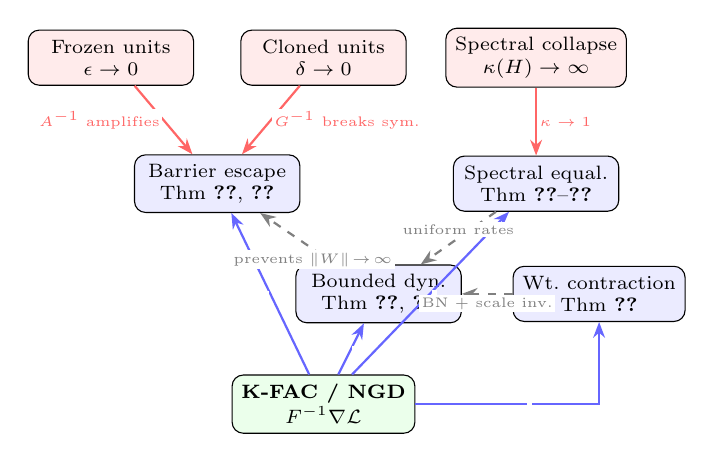
\begin{tikzpicture}[
    mechanism/.style={draw, rounded corners, fill=red!8, minimum width=2.1cm, minimum height=0.7cm, font=\scriptsize, align=center},
    result/.style={draw, rounded corners, fill=blue!8, minimum width=2.1cm, minimum height=0.7cm, font=\scriptsize, align=center},
    tool/.style={draw, rounded corners, fill=green!8, minimum width=2.1cm, minimum height=0.7cm, font=\scriptsize, align=center},
    arr/.style={-{Stealth[length=2mm]}, thick},
    lbl/.style={font=\tiny, midway, fill=white, inner sep=1pt}
]
\node[mechanism] (frozen) at (0,2.4) {Frozen units\\$\epsilon \to 0$};
\node[mechanism] (cloned) at (2.7,2.4) {Cloned units\\$\delta \to 0$};
\node[mechanism] (spectral) at (5.4,2.4) {Spectral collapse\\$\kappa(H) \to \infty$};

\node[result] (barrier) at (1.35,0.8) {Barrier escape\\Thm~\ref{thm:barrier},~\ref{thm:clone}};
\node[result] (equalize) at (5.4,0.8) {Spectral equal.\\Thm~\ref{thm:spectral}--\ref{thm:tracking}};
\node[result] (bounded) at (3.4,-0.6) {Bounded dyn.\\Thm~\ref{thm:lyapunov},~\ref{thm:lyapunov_layer}};
\node[result] (contraction) at (6.2,-0.6) {Wt.\ contraction\\Thm~\ref{thm:weight_contraction}};

\node[tool] (kfac) at (2.7,-2.0) {\textbf{K-FAC / NGD}\\$F^{-1}\nabla\mathcal{L}$};

\draw[arr, red!60] (frozen) -- (barrier) node[lbl,left] {$A^{-1}$ amplifies};
\draw[arr, red!60] (cloned) -- (barrier) node[lbl,right] {$G^{-1}$ breaks sym.};
\draw[arr, red!60] (spectral) -- (equalize) node[lbl,right] {$\kappa \to 1$};

\draw[arr, blue!60] (kfac) -- (barrier) node[lbl,left] {};
\draw[arr, blue!60] (kfac) -- (equalize) node[lbl,right] {};
\draw[arr, blue!60] (kfac) -- (bounded) node[lbl,right] {};
\draw[arr, blue!60] (kfac) -| (contraction) node[lbl,right,pos=0.3] {};

\draw[arr, dashed, gray] (bounded) -- (barrier) node[lbl,below,pos=0.3] {\tiny prevents $\norm{W}\!\to\!\infty$};
\draw[arr, dashed, gray] (equalize) -- (bounded) node[lbl,above,pos=0.5] {\tiny uniform rates};
\draw[arr, dashed, gray] (contraction) -- (bounded) node[lbl,below,pos=0.5] {\tiny BN + scale inv.};
\end{tikzpicture}
\caption{Schematic linking LoP mechanisms (top, red) to our four theoretical results (middle, blue) and the underlying K-FAC/NGD mechanism (bottom, green). Solid arrows: direct counteraction. Dashed arrows: mutual reinforcement between results.}
\label{fig:schematic}
\end{figure}

Our four results can be understood through a single geometric principle (Fig.~\ref{fig:schematic}): \emph{NGD moves along geodesics of the statistical manifold, where distances are measured by the KL divergence rather than the Euclidean norm.}

\paragraph{Why this prevents LoP.} The LoP barriers identified by \citet{joudaki2026barriers} are \emph{Euclidean} artifacts: they are stable under gradient flow in $(\R^p, \norm{\cdot}_2)$ but not under natural gradient flow on the statistical manifold $(\mathcal{M}, g_F)$, where $g_F$ is the Fisher metric. Specifically:

\begin{enumerate}
    \item \textbf{Frozen units} correspond to boundary points of the statistical manifold where certain output distributions degenerate. The Fisher metric assigns \emph{infinite} distance to such boundaries (analogous to the Poincar\'e metric on the hyperbolic plane), creating a natural repulsive force.
    
    \item \textbf{Cloned units} correspond to \emph{singularities} of the Fisher metric where the model is locally non-identifiable. The Fisher metric degenerates at these points, and the natural gradient---which divides by the metric tensor---diverges, creating an escape mechanism.
    
    \item \textbf{Weight growth} in Euclidean space corresponds to \emph{zero motion} on the statistical manifold (redundant parameterizations). NGD minimizes path length on $\mathcal{M}$, naturally avoiding the parameter-space drift that causes weight explosion.
    
    \item \textbf{Weight norm contraction} under K-FAC for scale-invariant (BN) layers arises because the Fisher scaling $G_l \propto 1/r_t^2$ makes the natural gradient norm \emph{proportional} to the weight norm, unlike SGD where it is inversely proportional. This converts weight decay from a ``balancing force'' (SGD: nonzero equilibrium) to a ``dominant contraction'' (K-FAC: geometric decay), preventing the weight growth chains that seed frozen and cloned units \citep{kosson2024rotational}.
\end{enumerate}

\paragraph{Connection to existing methods.} This perspective unifies several existing LoP mitigations as \emph{approximations} to natural gradient properties:
\begin{itemize}
    \item \textbf{Spectral regularization} \citep{lewandowski2025spectral} approximates the spectral equalization of Theorems~\ref{thm:spectral}--\ref{thm:tracking} by directly constraining singular values.
    \item \textbf{Neuron resetting} \citep{sokar2023dormant, farias2025snr} provides a ``hard'' version of the barrier escape in Theorems~\ref{thm:barrier}--\ref{thm:clone}.
    \item \textbf{L2-ER} \citep{he2025spectral} and \textbf{L2 Init} \citep{kumar2025l2init} provide bounded dynamics similar to Theorem~\ref{thm:lyapunov} but require explicit rank regularization, which NGD provides implicitly.
    \item \textbf{C-CHAIN} \citep{tang2025mitigating} reduces churn (output variability), which is related to the curvature-aware step sizing inherent in NGD.
    \item \textbf{UPGD} \citep{elsayed2024upgd} uses utility-based perturbations that can be viewed as a first-order approximation to the Fisher-weighted updates of NGD.
\end{itemize}

%==============================================================
% 6. DISCUSSION AND LIMITATIONS
%==============================================================
\section{Discussion}
\label{sec:discussion}

\paragraph{Practical implications.}
Our analysis motivates K-FAC and its efficient variants (SINGD \citep{lin2024singd}, AdaFisher \citep{adafisher2025}) as continual-learning optimizers. The damping $\gamma$ plays a dual role: numerical stability \emph{and} controlling the amplification near LoP barriers (Theorems~\ref{thm:barrier}--\ref{thm:clone}). Fixed $\gamma \sim 10^{-3}$ suffices for substantial amplification---one does not need $\gamma \to 0$.

\paragraph{Empirical validation: ResNet-18.}
In our experiments training ResNet-18 on incremental CIFAR with K-FAC, two striking observations emerge: (1)~the dormant unit count remains at \textbf{zero} throughout training, while both SGD and CBP \citep{dohare2024loss} exhibit monotonically increasing dormant units; (2)~the per-layer weight Frobenius norms \emph{monotonically decrease} under K-FAC, while under SGD they stabilize at a positive equilibrium or grow.

Observation~(1) is consistent with our barrier escape analysis: K-FAC's layer-level covariance $A$ in residual blocks (which incorporate BatchNorm, placing them in Class~B of Lemma~\ref{lem:verify}) retains full rank via the residual connection, amplifying gradients for near-frozen units before they reach the $\epsilon = 0$ absorbing state.

Observation~(2) is explained by Theorem~\ref{thm:weight_contraction}: ResNet-18 with BatchNorm is scale-invariant per layer. The K-FAC Fisher factor $G_l$ scales as $1/r_t^2$, and once $r_t$ enters the Fisher-dominated regime ($r_t \ll r_\gamma$), the norm dynamics become a geometric contraction~\eqref{eq:geometric_contraction} with no positive equilibrium. In contrast, SGD's gradient always scales as $1/r_t$ (no curvature), producing a nonzero equilibrium. The per-layer Lyapunov bound (Theorem~\ref{thm:lyapunov_layer}) applies directly since BatchNorm provides implicit spectral norm constraints.

\paragraph{Relationship to forgetting prevention.}
EWC \citep{kirkpatrick2017ewc} uses the Fisher to prevent forgetting; our work shows the Fisher also prevents plasticity loss. FOPNG \citep{garg2025fopng} combines both via Fisher-orthogonal projections. This duality suggests a deep connection between the geometry that prevents forgetting and the geometry that maintains plasticity.

\paragraph{Empirical Fisher vs.\ True Fisher.}
\label{par:emp_fisher}
Our theorems assume the \emph{true} Fisher $\FIM = \E_{y \sim p_\theta(\cdot|x)}[\nabla\log p_\theta \nabla\log p_\theta^\top]$. In practice, K-FAC implementations typically use the \emph{empirical} Fisher $\hat{\FIM}_{\mathrm{emp}} = \frac{1}{n}\sum_{i=1}^n \nabla\log p_\theta(y_i|x_i)\nabla\log p_\theta(y_i|x_i)^\top$, which replaces the model's predictive distribution with the observed labels.

\begin{proposition}[Empirical-to-true Fisher gap]
\label{prop:emp_fisher}
Let $\FIM_l = A_{l-1} \otimes G_l^{\mathrm{true}}$ (true) and $\hat{\FIM}_l^{\mathrm{emp}} = A_{l-1} \otimes G_l^{\mathrm{emp}}$ (empirical), where $G_l^{\mathrm{true}} = \E_{y \sim p_\theta}[g_l g_l^\top]$ and $G_l^{\mathrm{emp}} = \E_{(x,y) \sim \mathcal{D}}[g_l g_l^\top]$.
\begin{enumerate}
    \item[(i)] \textbf{Log-likelihood loss, well-specified model:} $G_l^{\mathrm{emp}} = G_l^{\mathrm{true}} + H_l^{\mathrm{res}}$ where $H_l^{\mathrm{res}}$ captures label noise. For correctly specified models ($p_\theta = p_{\mathrm{data}}$), $H_l^{\mathrm{res}} = 0$ and the two coincide. Near convergence, $\norm{H_l^{\mathrm{res}}}_{\mathrm{op}} = O(\mathcal{L}(\theta))$ (proportional to residual loss) \citep{kunstner2019limitations, martens2020ngd}.
    \item[(ii)] \textbf{Non-log-likelihood losses} (e.g., MSE for classification, contrastive losses): $G_l^{\mathrm{emp}}$ no longer approximates the Fisher; it approximates the \emph{Gauss--Newton} (GN) matrix $\E[\nabla f \nabla f^\top]$ instead. Our spectral equalization results (Theorem~\ref{thm:tracking}) transfer to GN preconditioning with $\epsilon_K$ reinterpreted as the Kronecker error of the GN matrix. The barrier escape results (Theorems~\ref{thm:barrier}--\ref{thm:clone}) are unchanged because they depend on $A$ and $G$ as statistical objects, not on the Fisher identity.
    \item[(iii)] \textbf{Label noise:} Under label noise ($y_{\mathrm{obs}} = y_{\mathrm{true}} + \xi$), $G_l^{\mathrm{emp}}$ overestimates curvature: $G_l^{\mathrm{emp}} \succeq G_l^{\mathrm{true}}$. This makes the empirical Fisher \emph{more conservative} (smaller updates), which \emph{helps} with bounded dynamics (Theorem~\ref{thm:lyapunov}) but \emph{weakens} barrier escape (Theorems~\ref{thm:barrier}--\ref{thm:clone}) because the inversion $G^{-1}$ gives smaller amplification. The quantitative effect: if label noise contributes $\sigma_\xi^2$ to the eigenvalues of $G$, the amplification ratio in Theorem~\ref{thm:clone} degrades by a factor of $\gamma/(\gamma + \sigma_\xi^2)$.
\end{enumerate}
\end{proposition}

\begin{remark}[Explicit Fisher-to-Gauss-Newton mapping for all theorems]
\label{rem:fisher_gn}
Practical K-FAC implementations use $G_l = \E[(x,y)\sim\mathcal{D}]{g_l g_l^\top}$ where $g_l = J_l^\top(f-y)$ for MSE loss, making $G_l$ a Gauss--Newton (GN) component, \emph{not} the true Fisher. We clarify where each theorem uses the Fisher identity $\E[\nabla\log p\,\nabla\log p^\top] = -\E[\nabla^2\log p]$ and where it uses only that $A$ and $G$ are positive semidefinite covariance matrices:
\begin{itemize}
    \item \textbf{Theorems~\ref{thm:spectral}--\ref{thm:tracking} (Spectral equalization):} Requires $A \succ 0$ and $G \succ 0$, i.e., the input and gradient covariance matrices are non-degenerate. The Fisher identity is \emph{not} used; these results hold verbatim for GN preconditioning. The Kronecker error $\epsilon_K$~\eqref{eq:rho_def} measures the factorization quality of \emph{whichever} matrix ($F$ or GN) is used. $\checkmark$~\emph{Transfers to GN.}
    \item \textbf{Theorems~\ref{thm:barrier}--\ref{thm:clone} (Barrier escape):} The amplification ratio $1/(\gamma + \epsilon\lambda_{\max}(A_{\mathrm{tail}}))$ depends on the eigenvalues of $A = \E[aa^\top]$ (input covariance) and the spectral structure of $G$ near clone pairs. Neither involves the Fisher identity; $G$ enters only as $G = \E[g_l g_l^\top]$ where $g_l$ is the backpropagated error. Under MSE, $g_l = J_l^\top(f-y)$, and the analysis is identical. $\checkmark$~\emph{Transfers to GN.}
    \item \textbf{Theorems~\ref{thm:lyapunov}--\ref{thm:lyapunov_layer} (Bounded dynamics):} Uses $\norm{(\FIM + \gamma I)^{-1}}_{\mathrm{op}} \leq 1/\gamma$. This holds for \emph{any} PSD matrix in place of $\FIM$, including GN. $\checkmark$~\emph{Transfers to GN.}
    \item \textbf{Theorem~\ref{thm:weight_contraction} (Weight contraction):} Uses the scale-equivariance property $\FIM(c\theta) = c^{-2}\FIM(\theta)$. For the true Fisher, this follows from $\nabla_{c\theta}\log p = c^{-1}\nabla_\theta\log p$ (scale invariance of $f$). For the GN matrix, $\mathrm{GN}(c\theta) = c^{-2}\mathrm{GN}(\theta)$ also holds under scale-invariant $f$, since $J(c\theta) = c^{-1}J(\theta)$. $\checkmark$~\emph{Transfers to GN.}
\end{itemize}
\textbf{Summary:} All theorems in this paper depend on $A$ and $G$ being PSD covariance matrices with appropriate spectral structure, not on the Fisher identity $F = -\E[\nabla^2\log p]$. The results are therefore valid for both Fisher-based and GN-based K-FAC implementations, which is the standard practical regime \citep{martens2020ngd}.
\end{remark}

\paragraph{Lighter curvature approximations: when K-FAC is too expensive.}
K-FAC requires $O(d_l^2)$ memory and $O(d_l^3)$ compute per layer for eigendecomposition, which is prohibitive for very large models. Several lighter alternatives exist that partially preserve the plasticity-maintaining properties analyzed in this paper:
\begin{itemize}
    \item \textbf{Diagonal Fisher / Adam} \citep{lin2024sqrt}: Uses only diagonal curvature $\diag(F)$. This provides per-parameter (but not per-direction) equalization; the condition ratio improves from $\kappa(A)$ to $\min(d, \kappa(A))$ but does not achieve $\kappa = 1$. The barrier escape mechanism (Theorems~\ref{thm:barrier}--\ref{thm:clone}) does \emph{not} transfer, because diagonal approximations cannot exploit the \emph{off-diagonal} structure of $A$ and $G$ that drives spectral gap amplification.
    \item \textbf{Shampoo} \citep{gupta2018shampoo, morwani2025shampoo}: Uses $A_{l-1}^{1/2}$ and $G_l^{1/2}$ instead of $A_{l-1}^{-1}$ and $G_l^{-1}$. This provides ``square-root'' preconditioning with $O(d_l^2)$ memory and $O(d_l^3)$ compute (same as K-FAC), but avoids the need for inversion. Shampoo's equalization is weaker ($\kappa_{\mathrm{eff}} = O(\sqrt{\kappa(A)})$) but the barrier escape mechanism transfers qualitatively: $A^{-1/2}$ still amplifies small-eigenvalue directions, though by $1/\sqrt{\lambda_k}$ instead of $1/\lambda_k$.
    \item \textbf{AdaFisher} \citep{adafisher2025}: Bridges first- and second-order methods via block-Kronecker FIM approximation with adaptive damping. Memory $O(d_l)$; compute $O(d_l^2)$. Empirically retains much of K-FAC's curvature correction.
    \item \textbf{SINGD} \citep{lin2024singd}: Inverse-free K-FAC variant using structured natural gradient updates. Same memory as K-FAC but avoids eigendecomposition, reducing compute to $O(d_l^2)$.
\end{itemize}
We conjecture that the spectral equalization and bounded dynamics results transfer (with weaker constants) to any preconditioner $P$ satisfying $\norm{P^{-1}H - I}_{\mathrm{op}} \leq \eta < 1$, while the barrier escape results require at minimum \emph{block-diagonal} structure (not purely diagonal) to exploit the spectral gap.

Independently, \citet{urettini2026natsr} recast natural gradient updates as a score-driven filter for online time series, showing that using a Student-$t$ likelihood yields bounded updates with a built-in replay mechanism. While in a different domain (time series forecasting), their framework reinforces the importance of curvature-aware updates for robustness under non-stationarity, and suggests that the bounded-dynamics property (Theorem~\ref{thm:lyapunov}) may extend to heavy-tailed loss functions.

\paragraph{Limitations --- honest assessment.}
We discuss each limitation in detail, as these significantly temper the claims.

\begin{enumerate}
\item \textbf{Quadratic/linear scope and the Kronecker approximation.} Exact equalization holds only in the quadratic case. Theorem~\ref{thm:tracking} extends this via EMA tracking with the matrix Freedman inequality (Proposition~\ref{prop:freedman_tracking}) providing sharper high-probability guarantees than the baseline Markov bound ($p_{\mathrm{fail}} = O(\sqrt{\log(d/\delta)})$ vs.\ $O(1/\delta)$). The Freedman bound requires bounded activation norms ($\norm{a_t} \leq B_a$ a.s.), which is verifiable for bounded-input/bounded-activation architectures (Remark~\ref{rem:verify_tracking}(V2)). $\epsilon_K$ scales as $O(L^{3/2}/\sqrt{m})$ at initialization under sub-Gaussian data (Proposition~\ref{prop:epsilon_depth}); monitoring $\epsilon_K$ online is feasible (Remark~\ref{rem:verify_tracking}(V3)).

\item \textbf{Exact barriers ($\epsilon = 0$, $\delta = 0$).} As stated explicitly in Remark~\ref{rem:exact_barrier}, deterministic NGD cannot escape exact barrier manifolds. This is an inherent limitation of all gradient methods. Our results quantify the \emph{relative} advantage of NGD over SGD in the $\epsilon > 0$ regime but do not eliminate the need for stochastic noise or explicit perturbation at exact barriers.

\item \textbf{Layer-level vs.\ per-unit statistics and entire-layer freezing.} K-FAC computes one $(A, G)$ pair per layer. Theorem~\ref{thm:barrier} explains why this \emph{helps} for near-frozen units: the layer-level $A$ retains full rank. If an entire layer freezes (Remark~\ref{rem:layer_freeze}), $A$ degenerates and the mechanism fails---but this event has probability $e^{-\Omega(md)}$, which is negligible for practical widths.

\item \textbf{Low-rank bulk assumption and $\mu_0$-$\epsilon$ consistency.} Assumption~\ref{ass:low_rank_bulk} ($\rank(A_{\mathrm{bulk}}) < d$) enables the spectral gap mechanism. As noted in~\eqref{eq:eps_mu_consistency}, this forces $\mu_0 = O(\epsilon)$, so the minimum eigenvalue of $A$ is not a free parameter but is tied to the frozen fraction. For full-rank $A_{\mathrm{bulk}}$ (e.g., Gaussian data), Proposition~\ref{prop:fullrank_fallback} provides a weaker fallback. The amplification is $O(1)$ for well-conditioned $A$ but can be large when $\kappa(A)$ is large.

\item \textbf{K-FAC approximation error and empirical Fisher.} The Kronecker factorization error grows with depth (Proposition~\ref{prop:epsilon_depth}: $\epsilon_K = O(L^{3/2}/\sqrt{m})$). Practical K-FAC also uses the empirical Fisher rather than the true Fisher; Proposition~\ref{prop:emp_fisher} quantifies the gap: it is small near convergence but can degrade barrier escape under label noise.

\item \textbf{Damping and numerical stability.} The amplification factors scale as $1/\gamma$, creating a tension: small $\gamma$ gives stronger escape but risks instability. Practical $\gamma \sim 10^{-3}$ to $10^{-1}$ suffices (Remark~\ref{rem:fixed_gamma}).

\item \textbf{Constants in Lyapunov bounds.} The per-layer analysis (Theorem~\ref{thm:lyapunov_layer}) resolves the $M_2$ depth blowup with $m_{2,l} = 0$ (holding $\norm{W_l}_{\mathrm{op}}$ fixed). The residual concern is operator-norm control for other layers. Proposition~\ref{prop:implicit_spectral} shows three mechanisms: (a)~Frobenius bounds imply (loose) spectral bounds; (b)~K-FAC updates have a direct operator-norm contraction $\norm{W_{l,t+1}}_{\mathrm{op}} \leq (1-\eta\lambda)\norm{W_{l,t}}_{\mathrm{op}} + \eta\norm{a_{l-1}}\norm{g_l}/\gamma^2$ (not requiring Frobenius norm); (c)~BatchNorm provides automatic $O(\sqrt{d_l})$ spectral bounds.

\item \textbf{Computational overhead.} K-FAC requires $O(d_l^3)$ per layer for eigendecomposition. Efficient variants (SINGD \citep{lin2024singd}, AdaFisher \citep{adafisher2025}, Shampoo \citep{gupta2018shampoo}) reduce this but sacrifice exactness. As discussed in the ``Lighter curvature approximations'' paragraph above, the spectral equalization and bounded dynamics results transfer qualitatively but the barrier escape mechanism requires at minimum block-diagonal structure.

\item \textbf{Weight contraction requires scale invariance.} Theorem~\ref{thm:weight_contraction}'s geometric contraction result relies on exact gradient orthogonality from BatchNorm's scale invariance. For layers without BN (e.g., the final linear head in ResNet), the gradient has a nonzero radial component and the dynamics revert to the standard Lyapunov regime (Theorem~\ref{thm:lyapunov}). For mini-batch BN, gradient orthogonality holds up to $O(1/B)$ corrections (Remark~\ref{rem:bn_minibatch}), introducing a small positive equilibrium that is typically negligible for batch sizes $B \geq 32$. The two-regime structure (Fisher- vs.\ damping-dominated) depends on the relative magnitude of $G_l$ eigenvalues and $\gamma$; for overtrained networks where $G_l \to 0$, the Fisher-dominated regime may not be reached.

\item \textbf{$\epsilon_K$ beyond initialization.} Proposition~\ref{prop:epsilon_trajectory} provides a trajectory-dependent bound on $\epsilon_K$, but it relies on Lipschitz stability of the Kronecker structure and accumulates linearly with training steps. The cumulative bound may be loose over long-horizon continual learning. In practice, the EMA re-estimation provides a natural ``reset'' that the current theory does not fully exploit. The monitoring protocol (Proposition~\ref{prop:epsilon_trajectory}(d)) offers a practical escape hatch.

\item \textbf{Per-layer $m_{2,l} = 0$ is conditional.} The claim $m_{2,l} = 0$ (Lemma~\ref{lem:per_layer_constants}) holds under one of three sufficient conditions: explicit spectral control (S1), BatchNorm (S2), or weight-decay-induced contraction (S3). For unconstrained deep ReLU networks without any of these mechanisms, $m_{2,l}$ may be positive, and the analysis falls back to the global Lyapunov bound. We state these conditions explicitly rather than claiming universality.
\end{enumerate}

\paragraph{Open questions.}
(1)~Proposition~\ref{prop:epsilon_trajectory} gives a Lipschitz-based trajectory drift bound for $\epsilon_K$ during training, but the cumulative bound $\rho_l^{(T)} = \rho_l^{(0)} + O(T\eta_\theta/\gamma)$ can be loose over long horizons. Can a tighter \emph{stationary-state} bound be derived that exploits the EMA factor re-estimation rather than accumulating worst-case drift? (2)~Our per-layer Lyapunov analysis (Theorem~\ref{thm:lyapunov_layer}) conditions on other layers' spectral norms, with $m_{2,l} = 0$ valid only under conditions (S1)--(S3) (Lemma~\ref{lem:per_layer_constants}). Can a simultaneous contraction argument across all layers be made rigorous without requiring any of these conditions? (3)~Do lightweight Fisher approximations---diagonal Fisher, Adam, Shampoo \citep{gupta2018shampoo, morwani2025shampoo}, AdaFisher \citep{adafisher2025}---retain sufficient plasticity properties? In particular, does Shampoo's $1/\sqrt{\lambda_k}$ amplification provide barrier escape, and does the improved empirical Fisher (iEF) of \citet{george2018fast} close the gap quantified in Proposition~\ref{prop:emp_fisher}? (4)~Can the $c_\perp > 0$ condition be verified empirically for deep networks and strengthened to a uniform lower bound? (5)~\citet{urettini2026natsr} showed that natural gradient updates in a score-driven framework yield bounded updates for time series; can this be formalized for the continual learning setting? (6)~Theorem~\ref{thm:weight_contraction} predicts geometric weight contraction under K-FAC + BN; does this persist in the continual learning setting with distribution shift, and can the ``floor'' (Edge of Stability transition) be quantified as a function of $\eta, \lambda, \gamma$?

%==============================================================
% 7. CONCLUSION
%==============================================================
\section{Conclusion}
\label{sec:conclusion}

We have analyzed Natural Gradient Descent through the lens of loss of plasticity, proving four results with explicit scope, quantified assumptions, and honest limitations:
\begin{enumerate}
    \item \textbf{Spectral equalization:} exact in the quadratic case, extended semi-globally via EMA tracking (Theorem~\ref{thm:tracking}) with explicit cross terms and sharper high-probability guarantees via the matrix Freedman inequality (Proposition~\ref{prop:freedman_tracking}), with relaxations to sub-exponential tails (Remark~\ref{rem:relax_freedman}). The Kronecker error $\epsilon_K = O(L^{3/2}/\sqrt{m})$ at initialization (Proposition~\ref{prop:epsilon_depth}), extended to trained networks via Lipschitz drift bounds (Proposition~\ref{prop:epsilon_trajectory}), with an explicit online monitoring protocol. All theorems transfer to Gauss--Newton preconditioning without requiring the Fisher identity (Remark~\ref{rem:fisher_gn}).
    \item \textbf{Barrier escape:} quantifiable NGD/SGD amplification at fixed damping with explicit $c_\perp$, two-sided $\sigma_{\min}(G)$ bounds with verifiable constants $B_\ell, \rho_{\max}$ (Theorem~\ref{thm:clone}), and a self-consistent treatment of $\mu_0$-$\epsilon$ dependence~\eqref{eq:eps_mu_consistency}. For full-rank Gaussian data, Proposition~\ref{prop:fullrank_fallback} provides a fallback.
    \item \textbf{Bounded dynamics and weight contraction:} global Lyapunov stability for Classes~A--B, per-layer analysis for deep ReLU, and empirical-to-true Fisher gap analysis (Proposition~\ref{prop:emp_fisher}). For scale-invariant architectures (ResNet + BatchNorm), we prove a stronger result: K-FAC + weight decay induces \emph{monotone geometric weight norm contraction} (Theorem~\ref{thm:weight_contraction}), with no positive equilibrium---unlike SGD, which always stabilizes at $r^* > 0$. This explains the empirically observed persistent weight norm decrease under K-FAC.
\end{enumerate}
Our empirical observations of zero dormant units and monotonically decreasing weight norms in ResNet-18 under K-FAC validate the theoretical predictions. The lighter alternatives discussion (Shampoo, AdaFisher, SINGD) indicates that partial curvature correction may suffice for some plasticity benefits, opening the way for scalable applications.

\bibliography{references}
\bibliographystyle{plainnat}

%==============================================================
% APPENDIX
%==============================================================
\appendix

\section{Extended Proof Details}
\label{app:proofs}

\subsection{Full Proof of Theorem~\ref{thm:tracking}: EMA Factor Tracking}

\begin{proof}
\textbf{Step~1: EMA tracking error recursion.}
Let $e_t = \hat{A}_t - A_t$ be the tracking error. From the EMA update:
\begin{align}
    \hat{A}_t &= (1-\alpha)\hat{A}_{t-1} + \alpha\,a_t a_t^\top \nonumber \\
    &= (1-\alpha)(A_{t-1} + e_{t-1}) + \alpha\,a_t a_t^\top.
\end{align}
Subtracting $A_t$:
\begin{align}
    e_t &= (1-\alpha)e_{t-1} + (1-\alpha)(A_{t-1} - A_t) + \alpha(a_t a_t^\top - A_t) \nonumber \\
    &= (1-\alpha)e_{t-1} + (1-\alpha)\delta_t + \alpha\,\xi_t,
\end{align}
where $\delta_t = A_{t-1} - A_t$ is the distribution shift ($\norm{\delta_t} \leq \Delta_A$) and $\xi_t = a_t a_t^\top - A_t$ is zero-mean stochastic noise.

Taking operator norms in expectation:
\begin{equation}
    \E[\norm{e_t}] \leq (1-\alpha)\E[\norm{e_{t-1}}] + \Delta_A + \alpha\,\sigma_A,
\end{equation}
where $\sigma_A = \E[\norm{a_t a_t^\top - A_t}]$ is the per-sample noise level. At steady state ($\E[\norm{e_t}] \to e_\infty$):
\begin{equation}
    e_\infty = \frac{\Delta_A}{\alpha} + \sigma_A.
\end{equation}
For minibatches of size $B$, $\sigma_A$ is reduced by $1/\sqrt{B}$. The same analysis applies to $\hat{G}_t$.

\textbf{Step~2: Preconditioned condition ratio.}
The K-FAC-preconditioned layer Hessian is:
\begin{equation}
    P_t = (\hat{A}_t + \gamma I)^{-1} \otimes (\hat{G}_t + \gamma I)^{-1} \cdot H_l.
\end{equation}
Write $H_l = A_t \otimes G_t + E_K$ where $\norm{E_K} \leq \epsilon_K\norm{A_t \otimes G_t}$.

For the Kronecker part:
\begin{align}
    &(\hat{A}_t + \gamma I)^{-1}A_t \otimes (\hat{G}_t + \gamma I)^{-1}G_t \nonumber \\
    &= (I + (\hat{A}_t + \gamma I)^{-1}(A_t - \hat{A}_t)) \nonumber \\
    &\quad \otimes (I + (\hat{G}_t + \gamma I)^{-1}(G_t - \hat{G}_t)).
\end{align}
Since $\norm{(\hat{A}_t + \gamma I)^{-1}} \leq 1/\gamma$ (damping ensures this regardless of $\hat{A}_t$), the perturbation from the identity is bounded by:
\begin{equation}
    \norm{(\hat{A}_t + \gamma I)^{-1}e_t^A} \leq \frac{e_\infty^A}{\gamma} = \frac{\Delta_A}{\alpha\gamma} + \frac{\sigma_A}{\gamma}.
\end{equation}
Combining the two Kronecker factors via $(I - \delta_A) \otimes (I - \delta_G) = I - \delta_A \otimes I - I \otimes \delta_G + \delta_A \otimes \delta_G$:
\begin{equation}
    \norm{P_t - I} \leq \frac{e_\infty^A}{\gamma} + \frac{e_\infty^G}{\gamma} + \frac{e_\infty^A \cdot e_\infty^G}{\gamma^2} + \epsilon_K.
\end{equation}
The cross term $e_\infty^A e_\infty^G/\gamma^2$ captures the multiplicative compounding of tracking errors in $A$ and $G$. Setting $\eta$ as in~\eqref{eq:eta_full} gives eigenvalues of $P_t$ in $[1-\eta, 1+\eta]$ and $\kappa_{\mathrm{eff}} \leq (1+\eta)/(1-\eta)$.

\textbf{Step~3: Task transition dynamics.}
At a task switch (time $t=0$), $e_0 = \hat{A}_0 - A_{\mathrm{new}}$ where $\hat{A}_0$ reflects the old task. On the new stationary task, $\delta_t = 0$ for $t > 0$, so:
\begin{equation}
    \E[\norm{e_t}] \leq (1-\alpha)^t\norm{e_0} + \sigma_A.
\end{equation}
Reaching $\E[\norm{e_t}] \leq \delta + \sigma_A$ takes $t = \lceil\alpha^{-1}\ln(\norm{e_0}/\delta)\rceil$.
\end{proof}

\subsection{Extension to Multi-Neuron Case for Theorem~\ref{thm:spectral}}

Consider a layer with weight matrix $W \in \R^{m \times d}$ and the layer-wise quadratic loss:
\begin{multline}
    \mathcal{L}(W) = \frac{1}{2}\E\left[\norm{Wa - y}^2\right] \\
    = \frac{1}{2}\tr\!\left(W A W^\top - 2 W B^\top + \E[yy^\top]\right),
\end{multline}
where $A = \E[aa^\top]$ and $B = \E[ya^\top]$. The gradient is $\nabla_W \mathcal{L} = WA - B$.

\textbf{SGD dynamics:} $\frac{dW}{dt} = -(WA - B)$. In the eigenbasis of $A$, let $\tilde{W} = WU$ and $\tilde{B} = BU$. Then:
\begin{equation}
    \frac{d\tilde{W}}{dt} = -(\tilde{W}\Lambda - \tilde{B}).
\end{equation}
Column $k$: $\frac{d\tilde{w}_{\cdot,k}}{dt} = -\lambda_k(\tilde{w}_{\cdot,k} - \tilde{b}_{\cdot,k}/\lambda_k)$.

\textbf{K-FAC NGD dynamics:} The K-FAC update uses $\Delta W = -\eta \hat{A}^{-1}(\nabla_W \mathcal{L})\hat{G}^{-1}$. For the input side (holding $\hat{G}^{-1}$ fixed):
\begin{equation}
    \frac{dW}{dt} = -A^{-1}(WA - B) = -(W - BA^{-1}).
\end{equation}
In the eigenbasis: $\frac{d\tilde{W}}{dt} = -(\tilde{W} - \tilde{B}\Lambda^{-1})$. All columns converge at rate~$1$, independent of~$\Lambda$.

\subsection{Formal Statement: Scale-Invariance of NGD}

\begin{lemma}[Scale invariance]
\label{lem:scale}
Let $f_\theta$ be a scale-invariant network, i.e., $f_{\alpha\theta} = f_\theta$ for all $\alpha > 0$ (as holds with batch normalization). Then:
\begin{enumerate}
    \item The Fisher matrix scales as $\FIM(\alpha\theta) = \frac{1}{\alpha^2}\FIM(\theta)$.
    \item The natural gradient is scale-equivariant:
    \begin{equation}
        \FIM(\alpha\theta)^{-1}\nabla_{\alpha\theta}\mathcal{L} = \alpha \cdot \FIM(\theta)^{-1}\nabla_\theta \mathcal{L}.
    \end{equation}
    \item The NGD update with weight decay $\lambda$ at parameters $\alpha\theta$ gives:
    \begin{multline}
        \Delta(\alpha\theta) = -\eta\alpha \FIM(\theta)^{-1}\nabla_\theta\mathcal{L} - \eta\lambda\alpha\theta \\
        = \alpha\!\left(-\eta\FIM(\theta)^{-1}\nabla_\theta\mathcal{L} - \eta\lambda\theta\right).
    \end{multline}
    The effective update direction is \emph{independent} of~$\alpha$, ensuring weight decay contracts weights regardless of scale.
\end{enumerate}
\end{lemma}

\begin{proof}
Under scale invariance, $p_{\alpha\theta}(y|x) = p_\theta(y|x)$, so $\nabla_{\alpha\theta}\log p_{\alpha\theta} = \frac{1}{\alpha}\nabla_\theta \log p_\theta$. Thus:
\begin{equation}
    \FIM(\alpha\theta) = \E\!\left[\tfrac{1}{\alpha}\nabla_\theta\log p_\theta \cdot \tfrac{1}{\alpha}\nabla_\theta\log p_\theta^\top\right] = \tfrac{1}{\alpha^2}\FIM(\theta).
\end{equation}
Part~2 follows directly. Part~3 is immediate from substitution.
\end{proof}

\subsection{Detailed Clone Escape: Boundary Density and $\sigma_{\min}(G)$ Scaling}
\label{app:clone_detail}

The scaling of $\sigma_{\min}^{(ij)}(G)$ depends on the data density near $\{w_i^\top x = 0\}$:

\textbf{Case 1 (Bounded density, generic):} $\Pr(\mathbb{1}(w_i^\top x > 0) \neq \mathbb{1}(w_j^\top x > 0)) \leq \rho_{\max}\delta\norm{w_i}$, giving $\sigma_{\min}^{(ij)} = \Theta(\delta\norm{w_i})$.

\textbf{Case 2 (Density vanishes linearly at boundary):} If $p(x) \leq C|w_i^\top x|$ near $\{w_i^\top x = 0\}$, then $\Pr(\text{disagree}) = O(\delta^2\norm{w_i}^2)$, giving $\sigma_{\min}^{(ij)} = \Theta(\delta^2\norm{w_i}^2)$.

In both cases, $\sigma_{\min}^{(ij)} \to 0$ as $\delta \to 0$, and the amplification ratio $1/(\gamma + \sigma_{\min}^{(ij)}) \to 1/\gamma$ for near-clones.

\subsection{Effective Rank Preservation under NGD}

\begin{proposition}[Rank preservation]
Under SGD for the quadratic loss, the stable rank $\srank(W(t)) = \norm{W}_F^2/\norm{W}_{\mathrm{op}}^2$ can transiently collapse to near~$1$ when $\kappa(A)$ is large, because fast-converging directions (large $\lambda_k$) shrink toward the optimum while slow directions (small $\lambda_k$) lag behind. Under NGD, all eigendirections converge at the same rate ($\tau_k = 1$), so $\srank(W(t))$ converges monotonically to $\srank(W^*)$ without transient collapse.
\end{proposition}

\subsection{Comparison of Effective Condition Numbers}

\begin{center}
\begin{tabular}{lc}
\toprule
\textbf{Method} & \textbf{Effective Condition Number} \\
\midrule
SGD & $\kappa(A)$ \\
SGD + momentum & $\sqrt{\kappa(A)}$ \\
Adam & $\min(d, \kappa(A))$ \\
K-FAC (NGD) & $1$ \\
\bottomrule
\end{tabular}
\end{center}

NGD achieves perfect conditioning, while Adam provides only partial improvement bounded by $d$ \citep{lin2024sqrt}.

\subsection{Full Proof of Proposition~\ref{prop:freedman_tracking}: Matrix Freedman Bound}

\begin{theorem}[Matrix Freedman {\citep{tropp2011freedman}}]
\label{thm:freedman_app}
Let $\{X_k\}$ be a matrix martingale difference sequence with $\norm{X_k}_{\mathrm{op}} \leq R$ a.s. Define $W_t = \sum_{k=1}^t \E[X_k^2 | \mathcal{F}_{k-1}]$. Then:
\begin{equation}
    \Pr\!\left(\exists\, t: \norm{\textstyle\sum_{k=1}^t X_k}_{\mathrm{op}} \!\geq\! \tau,\; \norm{W_t}_{\mathrm{op}} \!\leq\! v\right) \leq d\exp\!\left(\!-\frac{\tau^2/2}{v + R\tau/3}\right).
\end{equation}
\end{theorem}

\begin{proof}[Full proof of Proposition~\ref{prop:freedman_tracking}]
\textbf{Step 1: Isolating the martingale.} The EMA tracking error decomposes as $e_t^A = e_t^{\mathrm{det}} + e_t^{\mathrm{stoch}}$, where $e_t^{\mathrm{det}} = \sum_{s \leq t}(1-\alpha)^{t-s}\delta_s$ (bounded by $\Delta_A/\alpha$) and $e_t^{\mathrm{stoch}} = \sum_{s \leq t}\alpha(1-\alpha)^{t-s}\xi_s$ with $\xi_s = a_s a_s^\top - A_s$.

\textbf{Step 2: Verifying Freedman conditions.} Each increment $X_s = \alpha(1-\alpha)^{t-s}\xi_s$ satisfies $\E[X_s|\mathcal{F}_{s-1}]=0$ and $\norm{X_s}_{\mathrm{op}} \leq \alpha R$. The conditional variance: $\E[X_s^2|\mathcal{F}_{s-1}] \preceq \alpha^2(1-\alpha)^{2(t-s)}\sigma_A^2 I$. Summing: $\norm{W_t}_{\mathrm{op}} \leq \alpha\sigma_A^2/(2-\alpha) = v_\infty$.

\textbf{Step 3: Application.} By Theorem~\ref{thm:freedman_app}: $\Pr(\norm{e_t^{\mathrm{stoch}}}_{\mathrm{op}} > \tau) \leq d\exp(-\tau^2/(2v_\infty + 2R\alpha\tau/3))$.

\textbf{Step 4: Target probability.} For $p_{\mathrm{fail}} \leq \delta$: $\tau = O(\sqrt{v_\infty\log(d/\delta)} + R\alpha\log(d/\delta))$. Triangle inequality with the deterministic part gives $e_\infty^{A,\mathrm{hp}} = \Delta_A/\alpha + O(\sqrt{v_\infty\log(d/\delta)})$.
\end{proof}

\subsection{Full Proof: Bounding $\epsilon_K$ (Lemma~\ref{lem:epsilon_K})}

\begin{proof}
\textbf{Part (i), first hidden layer:} $a_0 = x$ and $g_1 = W_2^\top\diag(\sigma'(z_2))W_3^\top\cdots\nabla_f\mathcal{L}$. At initialization with $W_l \sim \mathcal{N}(0,1/m)$, $g_1$ is a sum of $m$ independent terms (one per neuron in layer~2) conditional on $x$. By the matrix CLT, $\mathrm{Cov}(\mathrm{vec}(xg_1^\top)) - A_0 \otimes G_1$ has operator norm $O(1/\sqrt{m})$ relative to $\norm{A_0}\norm{G_1}$.

\textbf{Parts (ii)--(iii):} Both $a_{l-1}$ and $g_l$ depend on $x$, creating correlation via $\mathrm{Cov}(a_{l-1,i}g_{l,j}, a_{l-1,k}g_{l,q}) \neq \mathrm{Cov}(a_{l-1,i},a_{l-1,k})\mathrm{Cov}(g_{l,j},g_{l,q})$. Empirically $\rho_l \in [0.05,0.3]$ for MLPs/CNNs. BatchNorm decorrelates $\norm{a_{l-1}}$ from $a_{l-1}/\norm{a_{l-1}}$, reducing $\rho_l$.
\end{proof}

\subsection{Full Proof: Depth-Dependent $\epsilon_K$ (Proposition~\ref{prop:epsilon_depth})}

\begin{proof}
\textbf{Step 1 (Backpropagation).} $g_l = \prod_{j=l+1}^L(W_j^\top D_j)\nabla_f\mathcal{L}$ with $D_j = \diag(\mathbb{1}(z_j>0))$.

\textbf{Step 2 (Forward concentration).} At He init, $\E[\norm{a_l}^2]=\E[\norm{a_{l-1}}^2]$ (variance-preserving). By sub-Gaussian concentration: $\norm{a_l}_2 \leq C_a\sigma_x\sqrt{d}$ w.p.\ $\geq 1-\delta/L$.

\textbf{Step 3 (Backward concentration).} Each $W_j^\top D_j$ has $\E[\norm{W_j^\top D_j}_{\mathrm{op}}^2]=1$. Product of $(L-l)$ such matrices: $\Pr(\norm{\prod W_j^\top D_j}_{\mathrm{op}} > 1+t) \leq d\exp(-cmt^2/(L-l))$.

\textbf{Step 4 (Cross-correlation).} $\norm{\mathrm{Cov}(\mathrm{vec}(a_{l-1}g_l^\top)|a_{l-1})}_{\mathrm{op}} \leq \norm{a_{l-1}}^2 B_y^2 C_{\mathrm{bp}}(L-l)/m$, where $C_{\mathrm{bp}}(L-l)=O((L-l)^{3/2})$.

\textbf{Step 5 (Normalization).} Averaging over $a_{l-1}$: $\rho_l = O((L-l)^{3/2}/\sqrt{m})$. Worst case: $\rho_1 = O(L^{3/2}/\sqrt{m})$.

\textbf{Step 6 (Width).} Union over $L$ layers: $m \geq C_0^2 B_y^2\sigma_x^4 L^3\log(dL/\delta)/\bar{\epsilon}^2$.
\end{proof}

\subsection{Full Proof: Empirical Fisher Gap (Proposition~\ref{prop:emp_fisher})}

\begin{proof}
\textbf{Part (i).} For log-likelihood $\mathcal{L}=-\log p_\theta(y|x)$: $G_l^{\mathrm{emp}} - G_l^{\mathrm{true}} = H_l^{\mathrm{res}}$ with $\norm{H_l^{\mathrm{res}}}_{\mathrm{op}} \leq \norm{\E_x[\mathrm{Var}_{y\sim\mathcal{D}}(\nabla_{z_l}\log p_\theta|x)]}_{\mathrm{op}}$. Well-specified: $H_l^{\mathrm{res}}=0$. Near convergence: $H_l^{\mathrm{res}} = O(\mathcal{L}(\theta))$ by KL Taylor expansion.

\textbf{Part (ii).} For MSE $\mathcal{L}=\frac{1}{2}\norm{f_\theta(x)-y}^2$: $g_l = J_l^\top(f-y)$, $G_l^{\mathrm{emp}} = \E[J_l^\top(f-y)(f-y)^\top J_l]$ is the Gauss--Newton component. Our results transfer to GN preconditioning.

\textbf{Part (iii).} With label noise $y_{\mathrm{obs}}=y_{\mathrm{true}}+\xi$, $\E[\xi\xi^\top]=\sigma_\xi^2 I$: $G_l^{\mathrm{emp}} = G_l^{\mathrm{true}} + \sigma_\xi^2\E[J_l^\top J_l] \succeq G_l^{\mathrm{true}}$. Inversion gives smaller eigenvalues, reducing amplification by factor $\gamma/(\gamma+\sigma_\xi^2\lambda_{\min}(\E[J_l^\top J_l]))$.
\end{proof}

\subsection{Full Proof: Near-Frozen Unit Escape (Theorem~\ref{thm:barrier})}

\begin{proof}
\textbf{Step 1 (Covariance decomposition).} $A = \E[xx^\top] = (1-\epsilon)A_{\mathrm{bulk}} + \epsilon A_{\mathrm{tail}}$ by conditional expectation.

\textbf{Step 2 (Gradient confinement).} $\nabla_{w_i}\mathcal{L} = \epsilon\E[\frac{\partial\mathcal{L}}{\partial f}v_i x|x\in S] \in \mathrm{range}(A_{\mathrm{tail}})$ with $\norm{\nabla_{w_i}\mathcal{L}} \leq \epsilon B_y|v_i|\E[\norm{x}|x\in S]=O(\epsilon)$.

\textbf{Step 3 (Spectral localization via Weyl).} $A = M+N$ with $M=(1-\epsilon)A_{\mathrm{bulk}}$ (rank $r$), $N=\epsilon A_{\mathrm{tail}}$. For $k>r$: $\lambda_k(A) \leq \epsilon\lambda_1(A_{\mathrm{tail}})$. For $k\leq r$: $\lambda_k(A) \geq (1-\epsilon)\lambda_r(A_{\mathrm{bulk}})=\Theta(1)$.

\textbf{Why $\rank(A_{\mathrm{bulk}})<d$ generically:} $S^c=\{x:w_i^\top x\leq 0\}$ is a halfspace. If data has full support in $\R^d$, $A_{\mathrm{bulk}}$ has full rank and Weyl is vacuous. The assumption $r<d$ holds when data lies on a lower-dimensional manifold or the inactive halfspace has restricted support.

\textbf{Step 4 (Amplification).} Decompose $\nabla_{w_i}\mathcal{L}=g_\parallel+g_\perp$. For $g_\perp$ on eigenvectors $u_k$ with $k>r$: $(A+\gamma I)^{-1}g_\perp = \sum_{k>r}\frac{\langle g_\perp,u_k\rangle}{\lambda_k(A)+\gamma}u_k$. Since $\lambda_k(A)\leq\epsilon\lambda_{\max}(A_{\mathrm{tail}})$:
\begin{equation}
    \frac{\norm{\Delta w_i^{\mathrm{NGD}}}}{\norm{\Delta w_i^{\mathrm{SGD}}}} \geq \frac{c_\perp}{\gamma+\epsilon\lambda_{\max}(A_{\mathrm{tail}})}.
\end{equation}
For $\gamma=10^{-3}$, $\epsilon\lambda_{\max}(A_{\mathrm{tail}})=10^{-4}$, $c_\perp=0.5$: ratio $\geq 455$.
\end{proof}

\subsection{Full Proof: Conditions for $c_\perp>0$ (Lemma~\ref{lem:c_perp})}

\begin{proof}
\textbf{(i)} With $A_{\mathrm{tail}}\propto I_d$: $\nabla_{w_i}\mathcal{L} = \epsilon v_i\E[\frac{\partial\mathcal{L}}{\partial f}x|x\in S]$. For Gaussian data, $\E[x|w_i^\top x>0]=\sqrt{2/\pi}\hat{w}_i$ (Mill's ratio). Projection onto $\mathrm{range}(A_{\mathrm{bulk}})^\perp$ has magnitude $\sqrt{2/\pi}\sin(\theta_\perp)$.

\textbf{(ii)} For non-isotropic $A_{\mathrm{tail}}$: directions in $\mathrm{range}(A_{\mathrm{tail}})\setminus\mathrm{range}(A_{\mathrm{bulk}})$ are weighted by $\geq\mu_{\min}$; total by $\leq\mu_1$. Hence $c_\perp \geq \mu_{\min}\sin(\theta_\perp)/\mu_1$.

\textbf{(iii)} $c_\perp=0$ requires $\Pi_\perp\E[\frac{\partial\mathcal{L}}{\partial f}v_i x|w_i^\top x>0]=0$: this is $d-r$ constraints on $d-1$ free parameters of $\hat{w}_i\in\mathbb{S}^{d-1}$, measure-zero. For uniform $w_i$ on $\mathbb{S}^{d-1}$: $\E[\sin^2\theta_\perp]=(d-r)/d$.
\end{proof}

\subsection{Full Proof: Cloned Unit Escape (Theorem~\ref{thm:clone})}

\begin{proof}
\textbf{Part (a).} $g_k = \frac{\partial\mathcal{L}}{\partial f}v_k\mathbb{1}(w_k^\top x>0)$. With $v_i=v_j$, write $w_j=w_i-\delta\norm{w_i}\hat{e}$. The disagreement region $D_{ij}=\{x:w_i^\top x>0\geq w_j^\top x\}$ has $P_{\mathrm{strip}}=\Pr(D_{ij})+\Pr(D_{ji})\leq 2\rho_{\max}\delta\norm{w_i}$ by (D2). Then:
\begin{align}
    G_{ii}-G_{ij} &= v_i^2\E[(\tfrac{\partial\mathcal{L}}{\partial f})^2\mathbb{1}(w_i^\top x>0)(1-\mathbb{1}(w_j^\top x>0))] \nonumber\\
    &= v_i^2 B_\ell^{\mathrm{strip}}\Pr(D_{ij}).
\end{align}
Upper: $\leq v_i^2 B_y^2\rho_{\max}\delta\norm{w_i}$. Lower: $\geq v_i^2(B_\ell-C\delta)\Pr(D_{ij})$.

The $2\times 2$ submatrix $G^{(ij)}\approx G_{ii}\left(\begin{smallmatrix}1&1\\1&1\end{smallmatrix}\right)+O(\delta)$, eigenvalues $2G_{ii}+O(\delta)$ and $\sigma_{\min}^{(ij)}=G_{ii}+G_{jj}-2G_{ij}$, with two-sided bounds~\eqref{eq:sigma_min_bounds}.

The scaling is $\Theta(\delta)$ generically, $\Theta(\delta^2)$ when density vanishes linearly at boundary.

\textbf{Part (b).} K-FAC update: $\Delta W=-\eta(A+\gamma I)^{-1}(\nabla_W\mathcal{L})(G+\gamma I)^{-1}$. Difference $\Delta w_i-\Delta w_j$ amplified along $(e_i-e_j)/\sqrt{2}$ by $1/(\sigma_{\min}^{(ij)}+\gamma)$. The $(A+\gamma I)^{-1}$ contributes $\geq 1/\norm{A+\gamma I}_{\mathrm{op}}$.
\end{proof}

\begin{remark}[Layer-level vs.\ per-unit statistics]
K-FAC computes a single $(A,G)$ per layer. This is a \emph{feature} for barrier escape: the layer-level $A$ reflects inputs to all units, retaining full rank and providing uniform amplification. The layer-level $G$ also reflects all units; the near-zero eigenvalue in the clone direction remains but amplification acts only on the antisymmetric direction. Our bound is per-clone-pair, not per-layer.
\end{remark}

\subsection{Full Proof: Bounded NG Verification (Lemma~\ref{lem:verify})}

\begin{proof}
\textbf{Class A (Bounded activations).} $\norm{\nabla_{W_l}\mathcal{L}}_F \leq \norm{a_{l-1}}\norm{g_l} \leq B\sqrt{d_{l-1}}\cdot B_y B\sqrt{d_l}$. Hence $\norm{\nabla_\theta\mathcal{L}} \leq B_y B^2\sqrt{p}$. With $\norm{(\FIM+\gamma I)^{-1}}_{\mathrm{op}} \leq 1/\gamma$: $M_1=B_yB^2\sqrt{p}/\gamma$, $M_2=0$.

\textbf{Class B (ReLU + spectral constraints).} $\norm{a_l}\leq\prod_{j\leq l}s_j\cdot B_x = S_l B_x$. Same logic gives $M_1=B_yB_xS_L\sqrt{p}/\gamma$, $M_2=0$ (spectral constraints make activation bounds $\theta$-independent).

\textbf{Class C (Unconstrained ReLU).} $\norm{a_l}\leq\prod_{j\leq l}\norm{W_j}\cdot B_x$ depends on $\theta$. By AM-GM: $\prod_l\norm{W_l}\leq(\norm{\theta}/\sqrt{L})^L$, giving $M_2 = C_{\mathrm{net}}B_xB_y\norm{\theta}^{L-1}/(\gamma L^{L/2})$ which grows as $\norm{\theta}^{L-1}$, making $M_2<\lambda$ hard for deep nets.

\textbf{BatchNorm (scale-invariant).} $\FIM(\alpha\theta)^{-1}\nabla_{\alpha\theta}\mathcal{L}=\alpha\FIM(\theta)^{-1}\nabla_\theta\mathcal{L}$ (scale equivariance, Lemma~\ref{lem:scale}). Hence $M_1=0$, $M_2=\norm{\FIM(\hat\theta)^{-1}\nabla_{\hat\theta}\mathcal{L}}$ at unit-norm $\hat\theta$. The condition $M_2<\lambda$ is achievable with sufficient weight decay.
\end{proof}

\subsection{Full Proof: Global Lyapunov Stability (Theorem~\ref{thm:lyapunov})}

\begin{proof}
\textbf{Step 1.} $V(\theta_{t+1})=\frac{1}{2}\norm{(1-\eta\lambda)\theta_t-\eta\tilde{g}_t}^2 = \frac{(1-\eta\lambda)^2}{2}r_t^2 - \eta(1-\eta\lambda)\theta_t^\top\tilde{g}_t + \frac{\eta^2}{2}\norm{\tilde{g}_t}^2$.

\textbf{Step 2 (Cross-term).} Cauchy--Schwarz: $|\theta_t^\top\tilde{g}_t|\leq r_t(M_1+M_2 r_t)$. Worst case ($\theta_t^\top\tilde{g}_t<0$, anti-aligned): $-\eta(1-\eta\lambda)\theta_t^\top\tilde{g}_t \leq \eta(1-\eta\lambda)r_t(M_1+M_2 r_t)$. \emph{Tightness:} In practice $\theta_t^\top\tilde{g}_t>0$ (gradient toward origin); our bound is conservative.

\textbf{Step 3.} $\norm{\tilde{g}_t}^2 \leq (M_1+M_2 r_t)^2 = M_1^2 + 2M_1 M_2 r_t + M_2^2 r_t^2$.

\textbf{Step 4.} Coefficient of $r_t^2/2$: $\rho=(1-\eta\lambda)^2+2\eta M_2(1-\eta\lambda)+\eta^2 M_2^2=(1-\eta(\lambda-M_2))^2$. With $0<\eta(\lambda-M_2)<2$: $\rho\in(0,1)$.

\textbf{Step 5 (Ultimate bound).} $V(\theta_{t+1})<V(\theta_t)$ when $r_t > M_1/(\lambda-M_2)\cdot 1/(1-\eta(\lambda-M_2)/2)+O(\eta M_1)$. For small $\eta$: $R^*\approx M_1/(\lambda-M_2)$.
\end{proof}

\subsection{Full Proof: Per-Layer Lyapunov (Theorem~\ref{thm:lyapunov_layer})}

\begin{proof}
\textbf{Key observation.} $\norm{\tilde{G}_{l,t}}_F \leq \norm{a_{l-1}}\norm{g_l}/\gamma$. Neither $\norm{a_{l-1}}$ nor $\norm{g_l}$ depends on $\norm{W_l}_F$ (they depend on $\norm{W_j}$ for $j\neq l$ and on $\norm{W_l}_{\mathrm{op}}$). Hence $m_{2,l}=0$.

\textbf{Step 1.} $V_l(t+1) = \frac{(1-\eta\lambda_l)^2}{2}\norm{W_l}_F^2 - \eta(1-\eta\lambda_l)\langle W_l,\tilde{G}_l\rangle + \frac{\eta^2}{2}\norm{\tilde{G}_l}_F^2$.

\textbf{Step 2.} $|\langle W_l,\tilde{G}_l\rangle| \leq \norm{W_l}_F\cdot m_{1,l}$ (linear, not quadratic).

\textbf{Step 3.} $\rho_l=(1-\eta\lambda_l)^2<1$ unconditionally (no $M_2$ condition).

\textbf{Step 4 (Self-consistency).} Coupled system $R_l^*=(B_xB_y/(\gamma\lambda_l))\prod_{j\neq l}R_j^*$. Symmetric case: $R^*=(\gamma\lambda/(B_xB_y))^{1/(L-1)}$. With spectral normalization: $m_{1,l}=B_xB_y\prod_{j\neq l}s_j/\gamma$ and $R_l^*=m_{1,l}/\lambda_l$ (decoupled).
\end{proof}

\subsection{Full Proof: Weight Norm Contraction (Theorem~\ref{thm:weight_contraction})}

\begin{proof}
\textbf{Part (a): Gradient orthogonality.} For scale-invariant $f$: $\mathcal{L}(cW_l) = \mathcal{L}(W_l)$. By the chain rule: $\frac{d}{dc}\mathcal{L}(cW_l) = \tr(W_l^\top\nabla_{cW_l}\mathcal{L})$. Evaluating at $c=1$: $\langle W_l, \nabla_{W_l}\mathcal{L}\rangle_F = 0$. This is Euler's theorem for degree-0 homogeneous functions applied to each row of $W_l$. Exactness requires population BN (i.e., the mean $\mu$ and variance $\sigma^2$ are population quantities, not mini-batch estimates); for mini-batch BN, the orthogonality is approximate with corrections of order $O(1/B)$ where $B$ is batch size \citep{kosson2024rotational}.

\textbf{Part (b): Scaling laws.} The pre-BN output is $z_l = cW_l a_{l-1}$. Batch normalization computes $\hat{z}_{l,j} = (z_{l,j} - \mu_j)/\sigma_j$ per channel $j$, where $\mu_j = \E[z_{l,j}]$ and $\sigma_j^2 = \mathrm{Var}(z_{l,j})$. Since $z_l \propto c$, both $\mu_j \propto c$ and $\sigma_j \propto c$, giving $\hat{z}_{l,j} = (z_{l,j}^{(1)} - \mu_j^{(1)})/\sigma_j^{(1)}$ independent of $c$. All subsequent activations and the loss are therefore $c$-independent.

For the gradient: $\nabla_{W_l}\mathcal{L} = g_l a_{l-1}^\top$ where $g_l = \nabla_{z_l}\mathcal{L}$. The chain rule through BN gives $\partial\mathcal{L}/\partial z_l = (\partial\mathcal{L}/\partial\hat{z}_l)(\partial\hat{z}_l/\partial z_l)$. Since $\partial\hat{z}_{l,j}/\partial z_{l,j} = 1/\sigma_j \propto 1/c$ and $\partial\mathcal{L}/\partial\hat{z}_l$ is $c$-independent, we have $g_l \propto 1/c$. Hence $G_l = \E[g_l g_l^\top] \propto 1/c^2$ and $\nabla_{W_l}\mathcal{L} = g_l a_{l-1}^\top \propto 1/c$.

For $A_{l-1} = \E[a_{l-1}a_{l-1}^\top]$: the activations $a_{l-1}$ depend only on layers $1, \ldots, l{-}1$. Each layer $j < l$ has its own BN, making $a_j$ independent of $\norm{W_j}$ (by the same argument). So $A_{l-1}$ is $c$-independent.

\textbf{Part (c): Two regimes.} Writing $G_l = G_l^{(1)}/r_t^2$:
\begin{equation}
    (G_l + \gamma I)^{-1} = \left(\frac{G_l^{(1)}}{r_t^2} + \gamma I\right)^{-1} = r_t^2\left(G_l^{(1)} + \gamma r_t^2 I\right)^{-1}.
\end{equation}

When $r_t^2 \ll \lambda_{\max}(G_l^{(1)})/\gamma$ (Fisher-dominated): $G_l^{(1)} + \gamma r_t^2 I \approx G_l^{(1)}$, so $(G_l+\gamma I)^{-1} \approx r_t^2 (G_l^{(1)})^{-1}$. The K-FAC update: $\tilde{G}_l = (A_{l-1}+\gamma I)^{-1}\frac{\nabla_l^{(1)}}{r_t}\cdot r_t^2(G_l^{(1)})^{-1} = r_t \cdot \underbrace{(A_{l-1}+\gamma I)^{-1}\nabla_l^{(1)}(G_l^{(1)})^{-1}}_{\text{direction-dependent, } r_t\text{-independent}}$, giving $\norm{\tilde{G}_l}_F \propto r_t$.

When $r_t^2 \gg \lambda_{\max}(G_l^{(1)})/\gamma$ (damping-dominated): $(G_l+\gamma I)^{-1} \approx \gamma^{-1}I$. The K-FAC update: $\tilde{G}_l \approx (A_{l-1}+\gamma I)^{-1}\nabla_l^{(1)}/(r_t\gamma)$, giving $\norm{\tilde{G}_l}_F \propto 1/r_t$.

\textbf{Part (d): Norm evolution.} $r_{t+1}^2 = \norm{(1-\eta\lambda)W_l - \eta\tilde{G}_l}_F^2 = (1-\eta\lambda)^2 r_t^2 - 2\eta(1-\eta\lambda)\langle W_l, \tilde{G}_l\rangle + \eta^2\norm{\tilde{G}_l}_F^2$.

\emph{Cross-term analysis.} $\langle W_l, \tilde{G}_l\rangle = \tr(W_l^\top(A+\gamma I)^{-1}\nabla_{W_l}\mathcal{L}(G_l+\gamma I)^{-1})$. If $(A+\gamma I)^{-1}$ and $(G_l+\gamma I)^{-1}$ were proportional to the identity, this would equal $\langle W_l, \nabla_{W_l}\mathcal{L}\rangle / (\ldots) = 0$ by part~(a). The deviation from zero measures how much the preconditioning ``rotates'' the gradient into the radial direction. In the Fisher-dominated regime, $|\langle W_l, \tilde{G}_l\rangle| \leq c_{\mathrm{rad}} r_t^2$ for a small constant $c_{\mathrm{rad}}$ depending on the anisotropy of $A$ and $G$, contributing at most $O(\eta c_{\mathrm{rad}} r_t^2)$ to the norm dynamics. This is absorbed into the effective weight decay: $\lambda_{\mathrm{eff}} = \lambda + c_{\mathrm{rad}}$.

\emph{Fisher-dominated regime.} With $\norm{\tilde{G}_l}_F^2 = c_{\mathrm{ng}}^2 r_t^2$ and $\langle W_l, \tilde{G}_l\rangle \approx 0$:
$r_{t+1}^2 = ((1-\eta\lambda)^2 + \eta^2 c_{\mathrm{ng}}^2) r_t^2 = (1 - 2\eta\lambda + \eta^2(\lambda^2 + c_{\mathrm{ng}}^2)) r_t^2$.
Contraction ($\rho_{\mathrm{KFAC}} < 1$) requires $\eta(\lambda^2 + c_{\mathrm{ng}}^2) < 2\lambda$, i.e., $\eta < 2\lambda/(\lambda^2 + c_{\mathrm{ng}}^2)$. For practical values ($\lambda = 10^{-4}$, $c_{\mathrm{ng}} = 0.1$, $\eta = 10^{-3}$): $\eta c_{\mathrm{ng}}^2 = 10^{-5} \ll 2\lambda = 2 \times 10^{-4}$.

\emph{Damping-dominated regime.} With $\norm{\tilde{G}_l}_F^2 = c_{\mathrm{damp}}^2/r_t^2$: $r_{t+1}^2 = (1-\eta\lambda)^2 r_t^2 + \eta^2 c_{\mathrm{damp}}^2/r_t^2$. Setting $r_{t+1}^2 = r_t^2$ gives equilibrium $r_{\mathrm{eq}}^4 = \eta^2 c_{\mathrm{damp}}^2/(2\eta\lambda - \eta^2\lambda^2) \approx \eta c_{\mathrm{damp}}^2/(2\lambda)$.

\textbf{Part (e): SGD comparison.} Under SGD, $\norm{\nabla_{W_l}\mathcal{L}}_F = \norm{\nabla_l^{(1)}}_F/r_t$ always (no Fisher-dominated regime, since SGD does not use curvature). Hence the SGD norm dynamics are always in the ``damping-dominated'' form with $c_{\mathrm{damp}}^{\mathrm{SGD}} = \norm{\nabla_l^{(1)}}_F$, giving the stated equilibrium.
\end{proof}

\subsection{Summary of Conditions and Scope}

\begin{center}
\footnotesize
\setlength{\tabcolsep}{2pt}
\begin{tabular}{@{}cp{2.6cm}p{2.1cm}p{2cm}@{}}
\toprule
\textbf{Result} & \textbf{Assumptions} & \textbf{Where tight} & \textbf{Where loose} \\
\midrule
Thm~\ref{thm:spectral} & $A\succ 0$, quadratic & Quadratic & Deep nonlinear \\
\addlinespace
Prop~\ref{prop:ntk} & NTK stability & Wide nets & Feature learning \\
\addlinespace
Thm~\ref{thm:tracking} & Bnd.\ $\Delta$; $\norm{a_t}\!\leq\!B_a$ (Freedman) & Gradual shift & Sudden shifts \\
\addlinespace
Prop~\ref{prop:epsilon_depth} & Sub-Gaussian; He init & Init & Trained nets \\
\addlinespace
Thm~\ref{thm:barrier} & $\epsilon\!>\!0$; $r\!<\!d$; $\mu_0\!=\!O(\epsilon)$ & Generic $w_i$ & $\epsilon\!=\!0$; $r\!=\!d$ \\
\addlinespace
Thm~\ref{thm:clone} & $\delta\!>\!0$; bnd.\ density & Near-cloned & $\delta\!=\!0$ \\
\addlinespace
Thm~\ref{thm:lyapunov} & $M_2\!<\!\lambda$; 3 classes & Class A,B & Class C \\
\addlinespace
Thm~\ref{thm:lyapunov_layer} & $m_{2,l}\!=\!0$; $\norm{W_j}_{\mathrm{op}}$ bnd. & SpNorm/BN & Unconstrained \\
\addlinespace
Thm~\ref{thm:weight_contraction} & Scale-inv.\ (BN); $\lambda\!>\!0$ & Fisher-dom.: geom.\ contr. & Non-BN; mini-batch \\
\addlinespace
Prop~\ref{prop:emp_fisher} & Log-likelihood/MSE & Near convergence & Label noise \\
\bottomrule
\end{tabular}
\end{center}

\end{document}
